%\begin{filecontents}
%  @CONTROL{apsrev41Control,title="0"%,author="48",editor="1",pages="1",year="0"}
%\end{filecontents}
\RequirePackage[l2tabu, orthodox]{nag}
\RequirePackage{fixltx2e}
\RequirePackage{fix-cm}
\PassOptionsToPackage{pdftex,psdextra=true,
pdfversion=1.7,
pdfencoding=auto,
pdfnewwindow=true,
pdfusetitle=true,
psdextra=true,
%pdftoolbar=true,
%pdfmenubar=true,
bookmarks=true,
bookmarksnumbered=true,
bookmarksopen=true,
pdfpagemode=UseThumbs,
bookmarksopenlevel=1,
pdfpagelabels=false
}{hyperref}
\PassOptionsToPackage{usenames,dvipsnames}{xcolor}
\documentclass[aps,english,superscriptaddress,onecolumn,twoside,longbibliography,pra,floatfix,fleqn,nofootinbib]{revtex4-1}%


\usepackage[utf8]{inputenx}% for arXiv use encoding ansinew
\input{ix-utf8enc.dfu}
%\usepackage[utf8x]{inputenc}% for arXiv use encoding ansinew
%\usepackage{utf8mathlite}% custom style sheet for unicode-ish math
%\usepackage{newunicodechar}
%\newunicodechar{∫}{\int}
%\usepackage{unicode-math}
\usepackage[OT1]{fontenc}
\usepackage{ucs} %for unichar

\usepackage{amsfonts}
\usepackage{amssymb}
\usepackage{amsthm}
\usepackage[intlimits,fleqn]{amsmath}
%\usepackage{mathdots}
\usepackage{graphicx}%
\usepackage{placeins} %for FloatBarrier
\usepackage{afterpage} %for FloatBarrier in afterpage wrapper
%\usepackage{flushend}
%\usepackage{dblfloatfix}
\usepackage[normalem]{ulem} %for sout
\usepackage[raggedright,bf,nooneline]{subfigure}
\renewcommand{\thesubfigure}{\alph{subfigure}}
\usepackage{paralist}

%\usepackage{ellipsis}
\usepackage{float}% (not with floatrow)
\usepackage{wrapfig}
%\usepackage{floatrow}


\usepackage{setspace}
\usepackage{array}
\usepackage{ragged2e}%for justifying text in tables
\usepackage{tabularx}
\def\tabularxcolumn#1{m{#1}}
\usepackage{booktabs}
%\usepackage{tabulary}
\newcolumntype{R}{>{\raggedleft\arraybackslash}X}
\newcolumntype{C}{>{\centering\arraybackslash}X}
\newcolumntype{L}{>{\raggedright\arraybackslash}X}
\newcolumntype{J}{>{\justifying\arraybackslash}X}

\setcounter{MaxMatrixCols}{30}
\providecommand{\U}[1]{\protect\rule{.1in}{.1in}}
%EndMSIPreambleData
\newtheorem{theorem}{Theorem}
\newtheorem{acknowledgement}[theorem]{Acknowledgement}
\newtheorem{algorithm}[theorem]{Algorithm}
\newtheorem{axiom}[theorem]{Axiom}
\newtheorem{claim}[theorem]{Claim}
\newtheorem{conclusion}[theorem]{Conclusion}
\newtheorem{condition}[theorem]{Condition}
\newtheorem{conjecture}[theorem]{Conjecture}
%\newtheorem{corollary}[theorem]{Corollary}
\newtheorem{corollary}{Corollary}[theorem]
\newtheorem{criterion}[theorem]{Criterion}
\newtheorem{definition}[theorem]{Definition}
%\newtheorem{example}[theorem]{Example}
\newtheorem{exercise}[theorem]{Exercise}
\newtheorem{lemma}[theorem]{Lemma}
\newtheorem{notation}[theorem]{Notation}
\newtheorem{problem}[theorem]{Problem}
\newtheorem{prop}{Proposition}
\newtheorem{taut}{Tautology}
\newtheorem{remark}[theorem]{Remark}
\newtheorem{solution}[theorem]{Solution}
\newtheorem{summary}[theorem]{Summary}
%\newenvironment{proof}[1][Proof]{\noindent\textbf{#1.} }{\ \rule{0.5em}{0.5em}}

% hyperlink stuff
\usepackage[usenames,dvipsnames]{xcolor}
\definecolor{ultramarine}{RGB}{63, 0, 255}
\definecolor{medblue}{RGB}{0, 0, 100}
\definecolor{panblue}{RGB}{0,24,150}
\definecolor{carmine}{RGB}{150, 0, 24}
\usepackage[breaklinks=true]{hyperref}
\hypersetup{colorlinks,
linkcolor=carmine,
citecolor=medblue,
urlcolor=panblue,
anchorcolor=OliveGreen}
%\usepackage{url}
\usepackage{pdfpages}

\definecolor{purple}{RGB}{128,0,128}
\definecolor{PURPLE}{RGB}{128,0,128}
\definecolor{BLACK}{RGB}{0,0,0}
\definecolor{ultramarine}{RGB}{63, 0, 255}
\definecolor{medblue}{RGB}{0, 0, 100}
\definecolor{panblue}{RGB}{0,24,150}
\definecolor{carmine}{RGB}{150, 0, 24}
\definecolor{gray}{RGB}{150, 150, 150}

\newcommand{\purp}[1]{{\color{purple}{#1}\color{black}}}
\newcommand*{\mred}[1]{{\color{RawSienna}{\mathbf{#1}}}}
\newcommand*{\mblue}[1]{{\color{MidnightBlue}{\ensuremath{#1}}}}
\newcommand*{\mpurp}[1]{{\color{Plum}{\mathbf{#1}}}}
\newcommand*{\mgreen}[1]{{\color{OliveGreen}{\mathbf{#1}}}}
\newcommand*{\tred}[1]{{\color{carmine}{\textbf{#1}}}}
\newcommand*{\tblue}[1]{{\color{MidnightBlue}{\textbf{#1}}}}
\newcommand*{\tpurp}[1]{{\color{Plum}{\textbf{#1}}}}
\newcommand*{\tgreen}[1]{{\color{Sepia}{\textbf{#1}}}}

\newcommand{\quoteby}{\raise.17ex\hbox{$\scriptstyle\sim$}}

\usepackage{verbatim} %for comment command
\usepackage{units}% for nicefrac
\newcommand{\half}[1]{\nicefrac{#1}{2}}

%\usepackage{braket} %provide \bra and \Bra and \set and \Set etc...
%\newcommand{\brackets}[1]{\lbrace{#1\rbrace}}
%\newcommand{\brackets}{\Set}



\usepackage{microtype}
%\usepackage{MnSymbol}
%\usepackage{mathabx}

\usepackage[capitalise]{cleveref}
\Crefname{eqs}{Eqs.}{Eqs.}

\creflabelformat{eqs}{(#2#1#3)}
\crefrangelabelformat{equation}{(#3#1#4-#5#2#6)}
%\crefmultiformat{equation}{eqs.~(#2#1#3)}{ and~(#2#1#3)}{, (#2#1#3)}{ and~(#2#1#3)}
\Crefmultiformat{equation}{Eqs.~(#2#1#3}{,#2#1#3)}{,#2#1#3}{,#2#1#3)}
\crefrangelabelformat{eqs}{(#3#1#4-#5#2#6)}
\Crefmultiformat{eqs}{Eqs.~(#2#1#3}{,#2#1#3)}{,#2#1#3}{,#2#1#3)}
\Crefname{prop}{\textbf{Prop}.}{\textbf{Props}.}
\Crefname{taut}{\textbf{Taut}.}{\textbf{Tauts}.}
\Crefname{section}{Sec.}{Secs.}

%\Crefname{ineq}{Ineq.}{Ineqs.}
%\creflabelformat{ineq}{(#2#1#3)}
%\crefrangelabelformat{ineq}{(#3#1#4-#5#2#6)}
%\Crefmultiformat{ineq}{Ineqs.~(#2#1#3}{,#2#1#3)}{,#2#1#3}{,#2#1#3)}

%\Crefname{ineqs}{Ineqs.}{Ineqs.}
%\creflabelformat{ineqs}{(#2#1#3)}
%\crefrangelabelformat{ineqs}{(#3#1#4-#5#2#6)}
%\Crefmultiformat{ineqs}{Ineqs.~(#2#1#3}{,#2#1#3)}{,#2#1#3}{,#2#1#3)}

\newcounter{step}[section]
\newenvironment{step}[1][]{\refstepcounter{step}\par\medskip
   \noindent \textbf{Step~\thestep}\rmfamily#1}{\par\medskip\par}
%\newenvironment{step}[1][Step]{\noindent\textbf{#1.} }{\ \rule{0.5em}{0.5em}}
\Crefname{step}{Step}{Steps}
\creflabelformat{step}{#2#1#3}
\crefrangelabelformat{step}{#3#1#4-#5#2#6}
\Crefmultiformat{step}{Steps.~#2#1#3}{,#2#1#3}{,#2#1#3}{,#2#1#3}
\renewcommand{\thestep}{\arabic{step}}


\newcounter{example}[section]
\newenvironment{example}[1][]{\refstepcounter{example}\par\medskip
   \noindent \textbf{Example~\theexample}\rmfamily#1}{\par\medskip\par}
%\newenvironment{step}[1][Step]{\noindent\textbf{#1.} }{\ \rule{0.5em}{0.5em}}
\Crefname{example}{Exmpl.}{Exmpls.}
\creflabelformat{example}{#2#1#3}
\crefrangelabelformat{example}{#3#1#4-#5#2#6}
\Crefmultiformat{example}{Exmpls.~#2#1#3}{,#2#1#3}{,#2#1#3}{,#2#1#3}
\renewcommand{\theexample}{\arabic{example}}


\usepackage[intlimits,fleqn]{mathtools} %for mathclap and prescript and more. Learning to love this package. And DeclarePairDelimeter!
\DeclarePairedDelimiter{\ceil}{\lceil}{\rceil}
\DeclarePairedDelimiter{\floor}{\lfloor}{\rfloor}
\DeclarePairedDelimiter{\parens}{\lparen}{\rparen}
\DeclarePairedDelimiter{\parenths}{\lparen}{\rparen}
\DeclarePairedDelimiter{\abs}{\lvert}{\rvert}
\DeclarePairedDelimiter{\norm}{\lVert}{\rVert}
\DeclarePairedDelimiter{\braces}{\lbrace}{\rbrace}
\DeclarePairedDelimiter{\bracks}{\lbrack}{\rbrack}
\DeclarePairedDelimiter{\expec}{\langle}{\rangle}
\newcommand{\brackets}[1]{\braces*{#1}}

%\usepackage{nath} %automatically pair delimiters. Provides \inline and \displayed. Adjusts \frac and /

%\newcommand{\na}{\ensuremath{\mathring{a}}}
%\newcommand{\nb}{\ensuremath{\mathring{b}}}
%\newcommand{\nc}{\ensuremath{\mathring{c}}}
\newcommand{\na}{\ensuremath{\overline{a}}}
\newcommand{\nb}{\ensuremath{\overline{b}}}
\newcommand{\nc}{\ensuremath{\overline{c}}}

\newcommand{\naf}{\ensuremath{\lnot a}}
\newcommand{\nbf}{\ensuremath{\lnot b}}
\newcommand{\ncf}{\ensuremath{\lnot c}}

\newcommand{\n}[1]{\ensuremath{\overline{#1}}}
\newcommand{\ot}[1]{\ensuremath{\overline{#1}}}
\newcommand{\Nor}[1]{\operatorname{\mathsf{Nor}}\!\bracks*{#1}}

\newcommand{\larray}[1]{\ensuremath{\begin{array}{l}#1\end{array}}}
\newcommand{\lparens}[1]{\ensuremath{\parens*{\larray{#1}}}}
%\newcommand{\NamedFunction}[2]{\operatorname{\mathsf{#1}}\!\bracks*{#2}}
%\newcommand{\NamedFunction}[2]{\operatorname{\mathsf{#1}}\!\bracks*{\larray{#2}}}
\newcommand{\NamedFunction}[2]{\operatorname{\mathsf{#1}}\!\begin{bmatrix*}[l]#2\end{bmatrix*}}
%\newcommand{\SmallNamedFunction}[2]{\operatorname{\mathsf{#1}}\bracks{#2}}
\newcommand{\SmallNamedFunction}[3][]{{\operatorname{\mathsf{#2}}_{#1}}\bracks{#3}}

\newcommand{\nap}{\ensuremath{a'}}
\newcommand{\nbp}{\ensuremath{b'}}
\newcommand{\ncp}{\ensuremath{c'}}
\newcommand{\napp}{\ensuremath{a''}}
\newcommand{\nbpp}{\ensuremath{b''}}
\newcommand{\ncpp}{\ensuremath{c''}}

\newcommand{\p}[2][]{{p_{#1}}\parenths{#2}}
%\newcommand{\pdf}[1]{\operatorname{\mathsf{PDF}}\!\parenths{#1}}
\newcommand{\pdf}[2][]{{P_{#1}}\parenths{#2}}
\newcommand{\An}[2][]{{\mathsf{An}_{#1}}\parenths{#2}}
\newcommand{\Pa}[2][]{{\mathsf{Pa}_{#1}}\parenths{#2}}
\newcommand{\Ch}[2][]{{\mathsf{Ch}_{#1}}\parenths{#2}}
\newcommand{\subgraph}[2][]{{\operatorname{\mathsf{SubDAG}}_{#1}}\bracks{#2}}
\newcommand{\ansubgraph}[2][]{{\operatorname{\mathsf{AnSubDAG}}_{#1}}\bracks{#2}}
\newcommand{\pasubgraph}[2][]{{\operatorname{\mathsf{PaSubDAG}}_{#1}}\bracks{#2}}
\newcommand{\nodes}[1]{\SmallNamedFunction{Nodes}{#1}}
\newcommand{\aindep}{\ensuremath{\mathrel{\mathopen{\Lsh}{\scriptstyle\emptyset}\mathclose{\Rsh}}}}


%\newcommand{\subsim}[1]{\substack{\textstyle #1\\[-0.3ex]\sim}}
%\newcommand{\subsim}{\utilde}
%\def\subsim#1{\mathord{\vtop{\ialign{##\crcr
%$\hfil\displaystyle{#1}\hfil$\crcr\noalign{\kern1.5pt\nointerlineskip}
%$\hfil\tilde{}\hfil$\crcr\noalign{\kern1.5pt}}}}}
\newcommand{\subsim}[1]{\tilde{#1}}

\newcommand{\cramp}[1]{\ensuremath{\mathord{#1}}}
%\newcommand{\cramp}[1]{\ensuremath{\mathopen{}#1\mathclose{}}} oldway. New way is better.
\newcommand{\eql}{\cramp{=}}

\usepackage{bm}
\newcommand{\setlambda}{\bm{\lambda}}


%%%% Tobias: to mark my edits and stuff
\usepackage{showkeys}
\usepackage[draft]{fixme}
\newcommand{\btob}{\color{OliveGreen}}
\newcommand{\etob}{\color{black}}



\let\stdsection\section
%\renewcommand\section{\clearpage\stdsection}%every section new page


\begin{document}
%\preprint{ }
%\title{Transitivity of implication and causal structure}
\title{The Inflation DAG Technique for Causal Inference with Hidden Variables}
\author{Elie Wolfe}
\email{ewolfe@perimeterinstitute.ca}
\affiliation{Perimeter Institute for Theoretical Physics, Waterloo, Ontario, Canada, N2L 2Y5}
\author{Robert W. Spekkens}
\email{rspekkens@perimeterinstitute.ca}
\affiliation{Perimeter Institute for Theoretical Physics, Waterloo, Ontario, Canada, N2L 2Y5}
\author{Tobias Fritz}
\email{tobias.fritz@mis.mpg.de}
\affiliation{Perimeter Institute for Theoretical Physics, Waterloo, Ontario, Canada, N2L 2Y5}
\affiliation{Max Planck Institute for Mathematics in the Sciences, Leipzig, Saxony, Germany, 04103}
\date{\today}


\begin{abstract}
The fundamental problem of causal inference is to infer from a given probability distribution over observed variables, what causal structures, possibly incorporating hidden variables, could have given rise to that distribution. Given some candidate causal structure, it is therefore valuable to derive infeasibility criteria, such that %any distribution violating an infeasibility criterion cannot be realized from the given causal structure.
the hypothesis is not a feasible causal explanation whenever the observed distribution violates an infeasibility criterion.
The problem of causal inference via infeasibility criteria comes up in many fields. Special infeasibility criteria are Bell inequalities (which distinguish non-classical from classical distributions) and Tsirelson inequalities (which distinguish quantum from post-quantum distributions), and Pearl's instrumental inequality. All of these are limited to very specific causal structures. Analogues of such inequalities for more-general causal structures, i.e., necessary criteria for either classical or quantum distributions to be realizable from the structure, are highly sought after. 

We here introduce a technique for deriving such infeasibility criteria, applicable to any causal structure. It consists of first \textit{inflating} the causal structure and then translating weak constraints on the inflated structure into stronger constraints on the original structure. Moreover, we show how our technique can be tuned to yield either classical criteria (i.e., that may have quantum violations), or post-classical criteria (i.e., that hold even in the context of general probability theories), depending on whether or not the inflation implicitly broadcasts the value of a hidden variable. Concretely, we derive polynomial inequalities for the so-called Triangle scenario, and we show how all Bell inequalities also follow from our method. %analyze Pearl's instrumental inequality from our perspective. 
Furthermore, given both a causal structure and a specific probability distribution, our technique can be used to efficiently witness their inconsistency, even absent explicit inequalities. The inflation technique is therefore both relevant and practical for general causal inference tasks with hidden variables.

%We introduce a technique for deriving such inequalities which apply to any causal structure (with hidden variables). This class contains all Bell inequalities as special cases. Our technique consists of ``inflating'' the causal structure. We then translate weak constraints on the inflated structure into much stronger constraints on the original structure through ``deflation" and quantifier elimination. One can derive either classical causal infeasibility criteria (i.e. that have quantum violations), or criteria which hold even in the context of general probability theories, depending on whether the inflation relies on cloning the values of the hidden variables. Concretely, we derive polynomial inequalities for the so-called Triangle scenario, and we show how the well-known Bell inequalities also follow from our method.%analyze Pearl's instrumental inequality from our perspective. 
%Furthermore, our method can efficiently witness the incompatibility of a probability distribution with a given causal structure even absent explicit quantifier-free inequalities.

\end{abstract}
\maketitle
%In Ref.~\cite{WoodSpekkens}, the standard proof of Bell's theorem is presented in the language of causal inference.  In particular, the CHSH inequality emerges as a special case of what Pearl calls an ``instrumental inequality''.  Hardy's proof of Bell's theorem is quite different from the standard proof and the following question naturally arises: is there a generic tool for classical causal inference of which the Hardy argument can be considered a special case when applied to the M-shaped causal structure of the Bell experiment?

%To try and answer this question, we apply Hardy-type reasoning to the triangle causal structure, that is, the one with three observed variables, each pair of which have a common cause.  We show that this sort of reasoning does indeed facilitate causal inference in the case of the triangle causal structure, thereby lending some evidence to the notion that this style of argument has the potential to be generalized into a generic tool for classical causal inference.

\section{Introduction}
Given some hypothesis of causal structure, it is desirable to determine \tblue{infeasibility criteria}, i.e., observable constraints such that the their violation implies the invalidity of the hypothesis as an explanation for observational data. Causal infeasibility criteria are used in a wide variety of statistics application, from sussing out biological pathways to enabling machine learning \cite{pearl2009causality,spirtes2011causation,studeny2005probabilistic,koller2009probabilistic}. \purp{ADD SENTENCES ABOUT HOW OUR WORK CONTRIBUTES TO GENERAL CAUSAL INFERENCE TASKS.} The foundational role of causal structure in quantum information theory has only recently been appreciated \cite{WoodSpekkens,fritz2012bell,pusey2014gdag,BeyondBellII}.

In contexts other than quantum theory, the latent nodes in causal structures are generally taken to represent hidden variables. This is not fully general, however, so we apply the retronym\footnote{Retronym (noun): a modification of an original term to distinguish it from a later development \cite{retronym}.} ``classical", as in classical causal structure and classical causal inference. The classical distributions of a given causal structure are defined as those which arise from it while restricting the latent nodes to be arbitrary (classical) random variables. Quantum distributions, by contrast, are those which are realizable if the latent nodes in the causal structure are allowed to be quantum systems. We hereafter take all causal structures and probability distributions to be classical, except where explicitly stated otherwise.

From a physics perspective, therefore, tightly characterizing the set of observable probability distributions realizable from a causal structure is critical, in order to recognize and exploit the existence of distributions that can be realized quantumly but not classically. Few techniques are known for bounding this set of distributions which are simultaneously practical and applicable to general causal structures. Celebrated examples include the use of conditional independence relations (easy) \cite{pearl2009causality,spirtes2011causation,studeny2005probabilistic,koller2009probabilistic} and entropic inequalities (more advanced) \cite{fritz2013marginal,chaves2014novel,chaves2014informationinference}. In the presence of hidden variables, these criteria only rarely provide a tight characterization, and frequently fail to witness the non-classicality of quantum distributions.% Indeed, all the causal scenarios we shall consider here are instances where conventional causal compatibility criteria are found to be insufficient 

Distinguishing quantum from classical correlations has historically been achieved through the use of Bell inequalities \cite{bell1966lhvm,GisinFramework2012,scarani2012device,Brunner2013Bell,BancalDIApproach}. Bell inequalities, however, are limited to very special causal scenarios involving \emph{only one} latent common cause variable, i.e.~Bell scenarios. A Bell scenario is also very special in that its realizable distributions admit characterization by a finite set of linear inequalities (after conditioning on the setting variables), i.e.~its realizable distributions comprise a convex polytope \cite{GisinFramework2012,FritzDuality}. %The nonconvexity of distributions realizable from a general structure is explicitly evidenced here. 
Entirely new techniques, therefore, are required to derive quantum-sensitive infeasibility criteria for more general causal scenarios \cite{fritz2012bell,pusey2014gdag,BeyondBellII}. 

To this end, we here introduce a new technique, applicable to any causal structure, for deriving infeasibility criteria. This technique allows for, but is not limited to, the derivation of polynomial inequalities.
% We show how the no-broadcasting theorem governing quantum theory \cite{NoCloningQuantum1996,NoCloningGeneral2006} can be exploited in order to derive specifically quantum-sensitive infeasibility criteria.
These criteria are generally based on the \emph{broadcasting} of the values of a hidden variable, i.e.~the assumption that its value can be copied and broadcast at will. The no-broadcasting theorem from quantum theory shows that this is not valid in the non-classical case, and from our perspective this is the reason for the existence of quantum violations of Bell inequalities. Moreover, our technique can also be applied in order to derive criteria that must be satisfied for all distributions that can be generated with latent nodes that are states in quantum theory or any other general probabilistic theory, simply by not assuming the possibility of broadcasting.
% like Tsirelson inequalities \cite{Tsirelson1980,Brunner2013Bell}, i.e. constraints which are satisfied by all distributions realizable from a given quantum causal structure. 

%\section{Notation}
\section{Notation and Definitions}\label{sec:definitions}

We follow the convention that upper-case letters indicate random variables while lower-case letters indicate some particular value associated with the corresponding random variable. In this convention, for example, a student's score on some exam $X$ might depend probabilistically on the amount of sleep $S$. The logical proposition, or \tblue{event}, $X\cramp{=}x,S\cramp{=}s$ should be understood as ``the student scores $x$ on the exam with a duration of sleep equal to $s$''. Events may be written in lower-case-only shorthand, such as $x,s$ instead of $X\cramp{=}x,S\cramp{=}s$.

Similarly, we indicate probability distributions using upper-case $P$, whereas lower-case $p$ is used to indicate the probability of particular events. Thus $\pdf{X, Y}$ is the multivariate probability distribution over the random variables $\{X Y\}$, and $\p{x, y}$ denotes the joint probability of the two events $X\cramp{=}x$ \emph{and} $Y\cramp{=}y$. We often omit the comma and just write $\pdf{X Y}$ and $\p{x y}$, respectively.

% We choose to indicate logical negation by $\n{x}\coloneqq\SmallNamedFunction{Not}{x}$, such that $\n{x}$ references the possibility of \emph{any} outcome other than $x$, so that $\p{\n{x}}\coloneqq\p{X\cramp{\neq}x}=1-\p{X\cramp{=}x}$. This convention effectively coarse-grains the outcome space into just two possibilities: $x$ and $\n{x}$. %Logical conjunction is herein represented by default, such that $\p{x y}$ is the joint probability of the two events  $X\cramp{=}x$ \emph{and} $Y\cramp{=}y$. 

\color{red}

%We need to define several notions.

A causal model consists of a pair of objects: a causal structure and a set of parameters.  The causal structure is a directed acyclic graph (DAG).  Recall that a DAG $G$ consists of a set of nodes and directed edges (i.e., ordered pairs of nodes), which we denote by $\SmallNamedFunction{Nodes}{G}$ and $\SmallNamedFunction{Edges}{G}$ respectively.  Physically, each node in the DAG corresponds to a localized system and a directed edge between two nodes corresponds to there being a direct causal influence from one system to the other.  The parameters specify, for each root node, how the system corresponding to that node is prepared, and for each node that has parents in the DAG, the precise manner in which it causally depends on its parents.  If a DAG is denoted $G$ and the parameter values thereon are denoted $\mathcal{P}(G)$, then the corresponding causal model is the pair $C = (G,\mathcal{P}(G))$.  We shall also make use of the notation $\SmallNamedFunction{DAG}{C}$ for $G$ and $\SmallNamedFunction{ParamVals}{C}$ for $\mathcal{P}(G)$.

Our terminology for the causal relations between the nodes in a DAG is the standard one. The parents of a node $X$ in a given graph $G$ are defined as those nodes which have directed edges originating at them and terminating at $X$, i.e. $\Pa[G]{X} = \{\:Y\:|\:Y\to X\:\}$.  Similarly the children of a node $X$ in a given graph $G$ are defined as those nodes which have have directed edges originating at $X$ and terminating at them, i.e. $\Ch[G]{X} = \{\:Y\:|\: X\to Y\:\}$. If $\bm{U}$ is a set of nodes, then we put $\Pa[G]{\bm{U}} := \bigcup_{X\in\bm{U}} \Pa[G]{X}$ and $\Ch[G]{\bm{U}} := \bigcup_{X\in\bm{U}} \Ch[G]{X}$.  The \tblue{ancestors} of a set of nodes $\bm{U}$, denoted $\An{\bm{U}}$, are defined as those nodes which have a directed \emph{path} to some node in $\bm{U}$, including the nodes in $\bm{U}$ themselves. Equivalently, $\An{\bm{U}} := \bigcup_{n\in\mathbb{N}} \mathsf{Pa}^n(\bm{U})$, where $\mathsf{Pa}^n(\bm{U})$ is inductively defined via $\mathsf{Pa}^0(\bm{U}) := \bm{U}$ and $\mathsf{Pa}^{n+1}(\bm{U}) := \mathsf{Pa}(\mathsf{Pa}^n(\bm{U}))$. 

The subgraph of $G$ induced by restricting attention to the set of nodes $\bm{V}$ will be denoted $\subgraph[G]{\bm{V}}$.
It consists of the nodes $\bm{V}$ and the edges between pairs of nodes in $\bm{V}$ per the original graph. Of special importance to us is the 
\tblue{ancestral subgraph} of $\bm{V}$, denoted $\ansubgraph{\bm{V}}$, which is the minimal subgraph containing the full ancestry of $\bm{V}$, $\ansubgraph{\bm{V}}\coloneqq\subgraph{\An{\bm{V}}}$. 


In a {\em classical} causal model, the localized systems are random variables, and the parameters are conditional probabilities\footnote{Classical causal models will be the primary focus of this article. Nonetheless, there is a quantum generalization of the notion of a causal model that will feature in our discussions at the end of this article.  In a {\em quantum} causal model\cite{leifer2013conditionalstates}, the localized systems are types of quantum systems (specified by Hilbert space dimensionality), and the parameters are quantum operations.  Specifically, for each root node, the model specifies a unit-trace positive operator on the Hilbert space for that system and for each non-root node, the model specifies a trace-preserving completely-positive linear map from the operators on the Hilbert space of the parents of the system to the operators on the Hilbert space of the system.  Certain nodes in a quantum causal model may be considered classical, in which case all states and operations must be diagonal in some fixed basis on that system.  One can also generalize the notion of a causal model further still to the case of generalized probabilistic theories, as was done in Ref.~\cite{pusey2014gdag}.
}.
 %probabilities and conditional probabilities on these random variables.  
Specifically, for each node, the model specifies a conditional probability distribution over the values of the random variable associated to that node, given the values of the variables associated to its parents in the DAG.  (In the case of root nodes, the parents are the null set and the conditional probability distribution is simply a probability distribution.)
 %Specifically, for each root node, the model specifies a probability distribution over the values of the associated random variable, and for each non-root node, it specifies a conditional probability distribution over the values of the random variable associated to that node, given the values of the variables associated to its parents in the DAG.  
Denoting the conditional probability distribution associated to a node $A$ in the DAG $G$ by $\pdf{A|\Pa[G]{A}}$, we have
\begin{align}
\mathcal{P}(G) \equiv \{\pdf{A|\Pa[G]{A}}: A \in \SmallNamedFunction{Nodes}{G}\}.
\end{align}
%Note that the root nodes are included as those for which the parents are the null set and the conditional probability distribution is simply a probability distribution.

We now introduce the notion of \tblue{the inflation of a classical causal model}.  We describe what inflation means for the causal structure and the parameters in turn.  Let $C=(G,\mathcal{P}(G))$ denote the original causal model and $C'=(G',\mathcal{P'}(G'))$ its inflation.  We say that the DAG $G'$ is the inflation of the DAG $G$, and that the parameters $\mathcal{P'}(G')$ are the inflationary image of the parameters $\mathcal{P}(G)$.

We begin by defining the condition under which a DAG $G'$  is an inflation of a DAG $G$.

For each node of $G$, $G'$ may contain one or more copies of that node. If $A$ denotes a node in the DAG $G$ that has copies in $G'$, then we denote these copies by $A_1,\ldots, A_k$.  The variable that indexes the copies is termed the {\em copy-index}.
%, and a set of variables in $G'$ that differ only by copy-index are called a {\em copy set}.  
The necessary condition on $G'$ for being an inflation of $G$ is that the ancestral subgraph in $G'$ of a node $A_i$ is equivalent, under removal of the copy-index, to the ancestral subgraph in $G$ of the node $A$.  
When two objects (e.g.~nodes, sets of nodes, DAGs, etc\ldots) are the same up to copy-indices, then we use $\sim$ to indicate this.  For instance, we have $A_i\sim A_j\sim A$.  Given this notational convention, we can formalize the condition for $G'$ to be an inflation of $G$ as follows:
\begin{align}\label{eq:definflationDAG}
%\forall A \in \SmallNamedFunction{Nodes}{G}, ???\nonumber\\
G' \in\SmallNamedFunction{Inflations}{G} \quad\text{ iff }\quad \forall A_i\in \SmallNamedFunction{Nodes}{G'}:\; \ansubgraph[G']{A_i}\sim\ansubgraph[G]{A}.
\end{align}

To illustrate the notion of the inflation of a DAG, we consider the DAG of \cref{fig:TriMainDAG}, which is called the {\em Triangle scenario} (for obvious reasons) and which has been studied by many authors [\citealp{pusey2014gdag}~(Fig.~E\#8), \citealp{WoodSpekkens}~(Fig.~18b), \citealp{fritz2012bell}~(Fig.~3), \citealp{chaves2014novel}~(Fig.~6a), \citealp{Chaves2015infoquantum}~(Fig.~1a), \citealp{BilocalCorrelations}~(Fig.~8), \citealp{steudel2010ancestors}~(Fig.~1b), \citealp{chaves2014informationinference}~(Fig.~4b)]
%As an example, consider the Triangle scenario [\citealp{pusey2014gdag}~(Fig.~E\#8), \citealp{WoodSpekkens}~(Fig.~18b), \citealp{fritz2012bell}~(Fig.~3), \citealp{chaves2014novel}~(Fig.~6a), \citealp{Chaves2015infoquantum}~(Fig.~1a), \citealp{BilocalCorrelations}~(Fig.~8), \citealp{steudel2010ancestors}~(Fig.~1b), \citealp{chaves2014informationinference}~(Fig.~4b)]. The associated DAG, the shape of which explains the name, is depicted here in \cref{fig:TriMainDAG}. 
%The Triangle scenario is a correlation scenario in the sense of \citet{fritz2012bell}; see especially Sec. 2.3 there. 
Different inflations of the Triangle scenario are depicted in \cref{fig:TriFullDouble,fig:Tri222,fig:simpleinflation,fig:simplestinflation,fig:TriDagSubA2B1C1}.


Next, we turn to defining the condition under which a set of parameters $\mathcal{P'}(G')$ are the inflationary image of the set of parameters $\mathcal{P}(G)$. 

The condition is simply that for every node $A_i$ in $G'$, the manner in which $A_i$ causally depends on its parents within $G'$ must be the same as the manner in which $A$ causally depends on its parents within $G$.   Formally, 
\begin{align}\label{eq:funcdependences}
\forall A_i \in \SmallNamedFunction{Nodes}{G'}:\; \pdf{A_i| \Pa[G']{A_i}}=\pdf{A|\Pa[G]{A}},
\end{align}
where Eq.~\eqref{eq:definflationDAG} guarantees that $A_i \sim A$ and $\Pa[G']{A_i} \sim \Pa[G]{A}$.  Note that the operation of equipping a modified DAG with the same functional dependencies as the original one also appears in the \emph{do calculus} of~\citet{pearl2009causality}. \fxnote{adhesivity and non-Shannon-type ineqs}

%A causal model specifies the causal structure and the autonomous causal mechanisms.  
To sum up then, inflation is a mapping to a new causal structure wherein each given variable in the original causal structure may have counterparts in the inflation and {\em where the causal mechanisms in the inflation DAG are given by the corresponding autonomous causal mechanisms in the original DAG.}  The duplication of variables implies that causal mechanisms in the inflation DAG are not necessarily autonomous, but rather often coincide with one another.

In addition to the notion of a causal model, we define the notion of a causal hypothesis, which is a set of causal models consistent with a single DAG. Specifically, if $G$ is a DAG and $S$ is a set of parameter values  consistent with $G$ (i.e. a set of possibilities for the conditional probability distributions at each node of $G$), then $G$ and $S$ define a causal hypothesis, which we denote by $H_{G,S}$, and which we define formally as the following set of causal models:
\begin{align}
H_{G,S} \equiv \{ C \mid \SmallNamedFunction{DAG}{C}=G, \SmallNamedFunction{ParamVals}{C} \in S\}.
\end{align}
% (is this standard usage of the term "model"?  In physics, a model typically does not include a specification of the boundary conditions, or does it?)
We denote  the set of {\em all} parameter values consistent with $G$ by $S_{\rm full}$, so that $H_{G,{S_{\rm full}}}$ is simply the causal hypothesis that the DAG is $G$, that is, the hypothesis there exists {\em some} parameter values supplementing $G$ such that the observed data can be explained by the resulting causal model. 

A causal inference problem is one whose input is some observed data---a sample of the probability distribution over the observed variables or some coarse-grained properties thereof, such as a list of conditional independence relations---and whose output is a verdict on (or probabilistic inference about) whether a given causal hypothesis can explain the observed data.   The particular causal inference problem that is most widely studied is one wherein the causal hypothesis just concerns the DAG.  Nonetheless, some causal inference problems explore more refined causal hypotheses, incorporating constraints on how  certain nodes in the DAG functionally depend on their parents.  An example is the assumption of an additive noise model for certain causal influences: if observed variable $Y$ has an observed variable $X$ as a parent and also a latent variable $U$, then the noise is deemed additive if $Y=\alpha X + \beta U$ for some scalars $\alpha$ and $\beta$ [provide references].  More general constraints on the functional dependences have also been explored [provide references].  Another example of a constraint on the parameters is a constraint on the form of the probabilities distributions over the latent variables. 

The inflation DAG technique that we introduce allows questions about the viability of one causal hypothesis for certain observed data to be turned into questions about the viability of a different sort of causal hypothesis for an inflation of the observed data.

%defines a novel sort of constraint on the parameters of a causal model.  We pause to describe this constraint in general terms, before introducing the notion of inflation.  The sorts of causal structures that can arise in our inflation scheme have the property that necessarily there will be certain pairs of variables which have the same ancestral subgraph.  The constraint on the parameters is that the two conditional probability distributions describing how each variable of the pair depends on its parents are quantitatively equal to one another.  (To our knowledge, this sort of constraint has not been considered before in causal inference.)


Inflation maps a causal hypothesis $H_{G,S}$ for the observed data to a causal hypotheses $H_{G',S'}$ for the observed data on the injectable sets, where $G'$ and $S'$ satisfy:
\begin{itemize}
\item The DAG $G'$ is an inflation of the DAG $G$ 
\item $\forall A_i \in \SmallNamedFunction{Nodes}{G'} : \pdf{A_i| \Pa[G']{A_i}} \in S'$ only if $\pdf{A| \Pa[G]{A}} \in S$
\end{itemize}
Note that even if $S=S_{\rm full}$, so that the original causal hypothesis puts no constraints on the parameter values, one generally has $S'\ne S'_{\rm full}$, that is, the inflationary image of the full set of parameter values on $G$ is not the full set of parameter values on $G'$. Rather, $S'$ incorporates a nontrivial restriction on the parameters consistent with $G'$, namely, that if nodes $A_i$ and $A_j$ on $G'$ are copies of a single node $A$ on $G$,then the parameter values on $G'$ are constrained to satisfy $\pdf{A_i| \Pa[G']{A_i}}=\pdf{A_j|\Pa[G']{A_j}}$.

Finally, we can spell out how the inflation DAG technique is useful for causal inference.  Note, first of all, that for any sets of nodes $\bm{U}\in \SmallNamedFunction{Nodes}{G'}$ and   $\subsim{\bm{U}}\in \SmallNamedFunction{Nodes}{G}$,
\begin{align}\label{eq:coincidingdistrodef}
\text{if }\quad \ansubgraph[G']{\bm{U}}\sim\ansubgraph[G]{\subsim{\bm{U}}}\quad\text{then}\quad \pdf{\bm{U}}=\pdf{\subsim{\bm{U}}}.
\end{align}
This follows from the fact that the probability distributions over $\bm{U}$ and $\subsim{\bm{U}}$ depend only on their ancestral subgraphs and the parameters defined thereon, which by the definition of inflation are the same for $\bm{U}$ and for $\subsim{\bm{U}}$.

It is useful to have a name for a set of nodes in the inflation DAG, $\bm{U}\in \SmallNamedFunction{Nodes}{G'}$, such that one can find a corresponding set in the original DAG, $\subsim{\bm{U}}\in \SmallNamedFunction{Nodes}{G}$, which an equivalent ancestral subgraph.  
We call such sets \tblue{injectable},
\begin{align}\label{eq:definjectable}
\bm{U}\in\SmallNamedFunction{InjectableSet}{G'} \quad\text{ iff }\quad \exists \subsim{\bm{U}}\in \SmallNamedFunction{Nodes}{G}: \ansubgraph[G']{\bm{U}}\sim\ansubgraph[G]{\subsim{\bm{U}}}.
\end{align}
In \cref{fig:Tri222}, for example, $\brackets{A_1 B_1 C_1}$ is injectable because its ancestral subgraph is equivalent up to copy-indices to the ancestral subgraph of $\brackets{A B C}$ in the original DAG (which is just the full DAG), and  $\brackets{A_2 C_1}$ is injectable because its ancestral subgraph is equivalent to that of $\brackets{ A C}$ in the original DAG. 

Note that it is clear that a set of nodes in the inflation DAG can only be injectable if it contains at most one copy of any node from the original DAG.  Similarly, it can only be injectable if its ancestral subgraph also contains at most one copy of any node from the original DAG.  
Thus, in \cref{fig:Tri222}, $\brackets{A_1 A_2 C_1}$ is not injectable because it contains two copies of $A$, and $\brackets{A_2 B_1 C_1}$ is not injectable because its ancestral subgraph contains two copies of $Y$. 




%Inflation is a map from a causal hypothesis on a DAG G to a causal hypothesis on a DAG G', where both G' and the set of constraints on the parameters supplementing G' depend on G.  Note that nontrivial constraints on the causal hypothesis on G also get mapped under inflation into nontrivial constraints on the causal hypothesis on G'.  



%What follows from this definition?
%The idea is that at the level of distributions, this property guarantees that all copies of a node in the inflation DAG have the same distribution as the corresponding node in the original DAG \emph{if} the functional dependencies among the variables are taken to be the same.


 \color{black}

Our terminology for the causal relations between the nodes in a DAG is the standard one. The parents of a node $X$ in a given graph $G$ are defined as those nodes which have directed edges originating at them and terminating at $X$, i.e. $\Pa[G]{X} = \{\:Y\:|\:Y\to X\:\}$.  Similarly the children of a node $X$ in a given graph $G$ are defined as those nodes which have have directed edges originating at $X$ and terminating at them, i.e. $\Ch[G]{X} = \{\:Y\:|\: X\to Y\:\}$. If $\bm{U}$ is a set of nodes, then we put $\Pa[G]{\bm{U}} := \bigcup_{X\in\bm{U}} \Pa[G]{X}$ and $\Ch[G]{\bm{U}} := \bigcup_{X\in\bm{U}} \Ch[G]{X}$.  The \tblue{ancestors} of a set of nodes $\bm{U}$, denoted $\An{\bm{U}}$, are defined as those nodes which have a directed \emph{path} to some node in $\bm{U}$, including the nodes in $\bm{U}$ themselves. Equivalently, $\An{\bm{U}} := \bigcup_{n\in\mathbb{N}} \mathsf{Pa}^n(\bm{U})$, where $\mathsf{Pa}^n(\bm{U})$ is inductively defined via $\mathsf{Pa}^0(\bm{U}) := \bm{U}$ and $\mathsf{Pa}^{n+1}(\bm{U}) := \mathsf{Pa}(\mathsf{Pa}^n(\bm{U}))$. 

We refer to a pair of nodes which do not share any common ancestor as being \tblue{ancestrally independent}, for which we invent the notation $X\aindep Y$. Generalizing to sets, $\bm{U}\aindep \bm{V}$ indicates that no node in $\bm{U}$ shares a common ancestor with any node in $\bm{V}$, i.e.~$\An{\bm{U}}\cap\An{\bm{V}}=\emptyset$. It is possible for more than two sets to be ancestrally independent: the notation ${\bm{U}\aindep \bm{V}\aindep \bm{W}}$ should be understood as indicating that the ancestors of $\bm{U}$,$\bm{V}$, and $\bm{W}$ comprise three distinct non-overlapping sets, i.e.~$\bm{U}\aindep \bm{V}$ and $\bm{V}\aindep \bm{W}$ and $\bm{U}\aindep \bm{W}$.

Ancestral independence is equivalent to $d$-separation by the empty set \cite{pearl2009causality,spirtes2011causation,studeny2005probabilistic,koller2009probabilistic}. Therefore, for distributions that are Markov with respect to the DAG~\cite{pearl2009causality,spirtes2011causation,studeny2005probabilistic,koller2009probabilistic}, ancestral independence of nodes implies marginal independence of the random variables. For us, all distributions over the variables represented by the nodes of a DAG will be assumed Markov. Intuitively, we presume that no statistical correlation is possible without causal explanation. Thus if a DAG possesses the feature ${\bm{U}\aindep \bm{V}\aindep \bm{W}}$, we demand \color{red} [Isn't this implied by the definitions and therefore doesn't need to be demanded?] \color{black} factorization of the marginal distributions such that ${\pdf{\bm{U} \bm{V} \bm{W}} = \pdf{\bm{U}} \pdf{\bm{V}} \pdf{\bm{W}}}$.


$\subgraph[G]{\bm{V}}$ refers to the induced subgraph of $G$ on a set of nodes $\bm{V}$. It consists of the nodes $\bm{V}$ and the edges between pairs of nodes in $\bm{V}$ per the original graph. Of special importance to us is the %\tblue{parental subgraph}, $\pasubgraph[G]{\bm{V}}\coloneqq\subgraph{\bm{V}\bigcup\Pa{\bm{V}}}$, the subgraph on $\bm{V}$ and all the parents of $\bm{V}$. We also make use of the
\tblue{ancestral subgraph}, $\ansubgraph{\bm{V}}\coloneqq\subgraph{\An{\bm{V}}}$, which is the minimal subgraph containing the full ancestry of $\bm{V}$. 

%\purp{Only the parents matter, not full ancestry!!!! Inflation DAG defined in terms of PARENTAL subgraphs, ditto for mapping and coinciding distributions. Will fix shortly.}

%A \tblue{graph map} $f_{G\to H}$ from graph $G$ to graph $H$ is a function which takes every edge and node in $G$ to some edge or node respectively in $H$, such that $f_{G\to H}(G)=H$. A graph map is essentially a collection of rules about edges and nodes.

%A \tblue{node map} $f_{G,H}$ is a surjective function which maps nodes in graph $G$ to nodes in graph $H$. A node map should be thought of as a collection of rules about (some) of $\nodes{G}$. A node map is generically \emph{not} a graph map, i.e. $f(G)\neq H$. 
%A \tblue{complete node map} $f_{G,H}$ maps \emph{every} $X\in\nodes{G}$ to some node in $\nodes{H}$. While the domain of $f$ is the set of $\nodes{G}$ whenever $f$ is a complete node map, nevertheless the codomain of $f$ need only be a subset of $\nodes{H}$. 

%A \tblue{bijective node map} maps unique nodes of $G$ to unique nodes of $H$. %A bijective node map does not need to be complete; it may only explicitly dictate how a subset of $\nodes{G}$ are mapped respective to a subset of $\nodes{H}$.

%A \tblue{graph isomorphism} $\mbox{Iso}_{G,H}$ is both a complete bijective node map and a graph map which transforms $G$ to $H$. Both properties are required to be a graph isomorphism. That it to say, not only ${\mbox{Iso}}(G)=H$ but also every $X\in\nodes{G}$ is mapped to some unique $Y\in\nodes{H}$ in one-to-one correspondence.

%Node maps can be nested hierarchically: If the rules of map $f2$ are a subset of the rules of $f1$ then we say that $f2$ \tblue{respects} $f1$.

%A \tblue{graph isomorphism} $\mbox{Iso}_{H,G}$ is both a special bijective map between $\nodes{H}$ and $\nodes{G}$ such that $H$ is transformed into $G$ under the action of map, i.e. $\mbox{Iso}(H)=G$. If a graph isomorphism exists which maps $H$ to $G$ then we say that $H$ and $G$ are isomorphic.

%A \tblue{deflation map} $\mbox{Dmap}_{H,G}$ is a special surjective map between $\nodes{H}$ and $\nodes{G}$ such that ${\mbox{Dmap}\parenths*{\ansubgraph[H]{X}}=\ansubgraph[G]{\mbox{Dmap}\parenths*{X}}}$ for all $X\in\nodes{G'}$. If a deflation map exists from $\nodes{H}$ to $\nodes{G}$ then we say that $H$ is a valid \tblue{inflation} of $G$.

%A (connected) subgraph of $H$, say $H'$, is said to be a \emph{deflatable subgraph} if the deflation map acts \mbox{Dmap} to transform $H'$ into a subgraph of $G$, ${\mbox{Dmap}\parenths*{H'}\subseteq G}$. By the definition of inflation, the ancestral subgraph of any single node in $H$ is a deflatable subgraph.

%A set of nodes $\bm{U}$ is said to be a \emph{deflatable set} if its ancestral subgraph is deflatable, i.e. ${\mbox{Dmap}\parenths*{\ansubgraph[H]{\bm{U}}}=\ansubgraph[G]{\mbox{Dmap}\parenths*{\bm{U}}}}$. 



%\begin{theorem}
%$\mbox{Dmap}\parenths*{\ansubgraph[H]{X}}=\ansubgraph[G]{\mbox{Dmap}\parenths*{X}}$ for all $X\in\nodes{H}$ if and only if $\mbox{Dmap}\parenths*{\Pa[H]{X}}=\Pa[G]{\mbox{Dmap}\parenths*{X}}$ for all $X\in\nodes{H}$.
%\end{theorem}


%\begin{theorem}
%${\mbox{Dmap}\parenths*{\ansubgraph[H]{\bm{U}}}=\ansubgraph[G]{\mbox{Dmap}\parenths*{\bm{U}}}}$ if and only if $\An[H]{\bm{U}}$ is ``duplicate free", that is to say, no two nodes in $\An{\bm{U}}$ deflate to the same node in $G$.
%\end{theorem}


We now introduce the notion of an \tblue{inflation DAG}. The nodes of an inflation DAG are copies $A_1,\ldots,A_k$ of the nodes of the original DAG, where the subscript $i$ is just a dummy index of sorts, and such that the following defining property holds: \tred{upon removing the subscripts indexing the copies, the ancestral subgraph in $G'$ of a node $A_i$ looks like the ancestral subgraph of the corresponding node $A$ in $G$.} The idea is that at the level of distributions, this property guarantees that all copies of a node in the inflation DAG have the same distribution as the corresponding node in the original DAG \emph{if} the functional dependencies among the variables are taken to be the same.

%Intuitively, we may thing of a node in a DAG as a ``black box" system that outputs random signals. A directed edge from $U$ to $V$ is then analogous to a wire which takes some output from $U$ and passes it as input to $V$. Inflation consists of acting on the edges of the DAG in two possible ways:
%\begin{itemize}
%\item We can produce an arbitrary number of further copies of the output node  (resulting in new edges).
%\item We can produce independent copies of the input node node (resulting in new nodes).
%\end{itemize}

When two objects (e.g.~nodes, sets of nodes, DAGs, etc\ldots) are the same up to dummy indices, then we use $\sim$ to indicate this, so $A_i\sim A_j\sim A$. 
The formal definition of an inflation DAG is therefore as follows:
\begin{align}\label{eq:definflationDAG}
G'\in\SmallNamedFunction{Inflations}{G} \quad\text{ iff }\quad \forall_{A_i\in G'}\; \ansubgraph[G']{A_i}\sim\ansubgraph[G]{A}.
\end{align}


\begin{figure}[t]
\centering
\begin{minipage}[b]{0.23\linewidth}
\centering
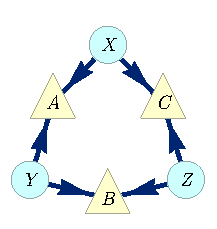
\includegraphics[scale=1]{TriDagRaw.pdf}
\caption{The causal structure of the Triangle scenario.}\label{fig:TriMainDAG}
\end{minipage}
\hfill
\begin{minipage}[t]{0.38\linewidth}
\centering
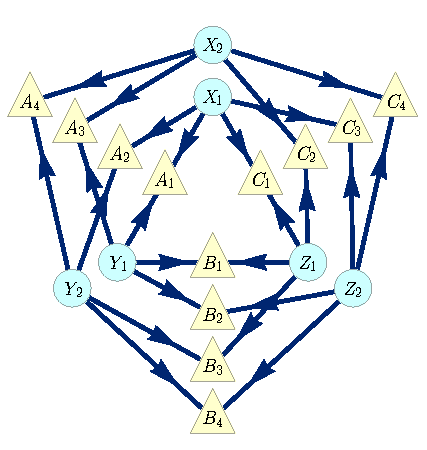
\includegraphics[scale=1]{TriDagFull222.pdf}
\caption{An inflation DAG of the Triangle scenario where each latent node has been duplicated, resulting in four copies of each observable node.}\label{fig:TriFullDouble}
\end{minipage}
\hfill
\begin{minipage}[b]{0.35\linewidth}
\centering
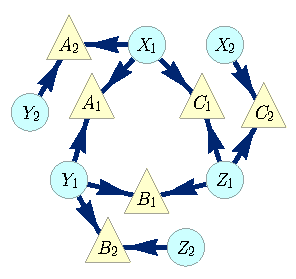
\includegraphics[scale=1]{TriDagSub222.pdf}
\caption{Another inflation of the Triangle scenario consisting, also notably $\ansubgraph[(\textrm{\cref{fig:TriFullDouble}})]{A_1 A_2 B_1 B_2 C_1 C_2}$.}\label{fig:Tri222}
\end{minipage}
\end{figure}


%To formally define an inflation DAG we first define the \tblue{deflation map}. The deflation map $\bm{\mbox{Dmap}}$ is the implicit function which maps the various $A_i$ to $A$, and it is generally a surjective function. Note that $\bm{\mbox{Dmap}}$ becomes bijective when restricted to the domain of any individual $A_i$. Now, an inflation DAG must posses the following recursive property:
%For every $\bm{U}$ such that $\bm{\mbox{Dmap}}$ acts bijectively when restricted to the domain $\bm{U}$ it must also be true that $\bm{\mbox{Dmap}}$ also acts bijectively when restricted to the domain of $\bm{U}\bigcup\Pa{\bm{U}}$. 
%Equivalently, $G'$ is a valid inflation DAG if and only if $\Pa[G']{A_i}\sim\Pa[G]{A}$ and $\An[G']{A_i}\sim\An[G]{A}$ for all $A$ and all $i$, where $\bm{U}\sim\bm{V}$ indicates one-to-one equivalence between $\bm{U}$ and $\bm{V}$ up to dummy indices.

As an example, consider the Triangle scenario [\citealp{pusey2014gdag}~(Fig.~E\#8), \citealp{WoodSpekkens}~(Fig.~18b), \citealp{fritz2012bell}~(Fig.~3), \citealp{chaves2014novel}~(Fig.~6a), \citealp{Chaves2015infoquantum}~(Fig.~1a), \citealp{BilocalCorrelations}~(Fig.~8), \citealp{steudel2010ancestors}~(Fig.~1b), \citealp{chaves2014informationinference}~(Fig.~4b)]. The associated DAG, the shape of which explains the name, is depicted here in \cref{fig:TriMainDAG}. 
%The Triangle scenario is a correlation scenario in the sense of \citet{fritz2012bell}; see especially Sec. 2.3 there. 
Two examples of inflations of the Triangle scenario are depicted in \cref{fig:TriFullDouble,fig:Tri222}.

%Possible inflations of the Triangle scenario are depicted in \cref{fig:TriFullDouble,fig:Tri222}; every copy of the random variable $A$ in an inflation has precisely two parents, one of which is a copy of the random variable $X$ and one of which is a copy of the random variable $Y$, just as in the original DAG. %The duplication of $Y$ into $Y_1$ and $Y_2$ leads to $X_1$ having outgoing edges to both $A_1$ and $A_2$ in \cref{fig:TriFullDouble,fig:Tri222}. Thus, inflating a DAG not only leads to duplicated nodes but to duplicated \emph{edges}. 



%In order for $G'$ to be a a ``valid" inflation of $G$ it must satisfy two properties:
%\begin{compactenum}
%\item There exists a \tblue{deflation map} $dmap$, i.e. a complete node map from the inflation DAG to the original DAG. $dmap$ takes every node $X\in\nodes{G'}$ to some node in $\nodes{G}$. To make this clear we demand that all those nodes $\bm{A}\in\nodes{G'}$ which map to $A$ in $G$ should \emph{share the name} $A$, and be distinguished only by dummy indices $A_1,A_2...$. Using this labelling, we find that $\forall_i \;{dmap}(A_i)\cramp{=}A$. The deflation map is surjective, and generally not bijective. We refer to the various $A_i$ as multiple \tblue{copies} of $A$ in the inflation DAG.
%\item For every node and every index $A_i$ in $G'$ it must be true that there exists an $f$-compatible graphical isomorphism between $\SmallNamedFunction{AnSubDAG}{A_i}$ (a subgraph of $G'$) and $\SmallNamedFunction{AnSubDAG}{A}$ (a subgraph of $G$). A graphical isomorphism is a bijective map between the nodes of $G'$ and the nodes of $G$ which also maps the (directed) edges in a one-to-one fashion. An isomorphism $Iso$ is $f$-compatible if $Iso(V_i)\to V$ for all $V_i \in \An{A_i}$.
%\item The deflation map must be a graph isomorphism at least when considering ancestral subgraphs within the inflation DAG. Formally: For all $X\in\nodes{G'}$ it must be true that $dmap\parenths*{\Pa[G']{X}}=\Pa[G]{dmap\parenths*{X}}$, i.e. the parents of every individual node in the inflation DAG $G'$ map bijectively to the corresponding parents of the mapped node in the original DAG $G$\footnote{This is reminiscent of covering spaces in topology.}. 
%\end{compactenum}

%The latter property is equivalent to $dmap\parenths*{\ansubgraph[G']{X}}=\ansubgraph[G]{dmap\parenths*{X}}$ for all $X\in\nodes{G'}$. In other words, each individual random variable in the inflated DAG has precisely the same causal history as it \emph{would have had} in the original DAG, up to the dummy indices indicating the deflation map. 

Any causal model for the original DAG specifies a corresponding causal model for the inflated DAG, by virtue of
\begin{align}\label{eq:funcdepends}
\forall_{A_i\in G'}\; \pdf{A_i|\Pa{A_i}}=\pdf{A|\Pa{A}},
\end{align}
where one identifies the parents of $A_i$ in $G'$ with the parents of $A$ in $G$. If a causal model on $G'$ is of this form, we call it an \tblue{inflation model}. In particular, all copies of exogenous (non-root) nodes in an inflation model share the same functional dependence on their parents, and all copies of endogenous (root) nodes in the inflated DAG are identically \emph{and independently} distributed. For us, the most relevant feature of an inflation model is that all the copies of a single random variable can have the same probability distribution as the corresponding variable in the original DAG,
% Implicit constraints are embedded into every inflation DAG which restrict the sorts of causal models compatible with the inflation DAG. 
%This follows from assuming that each copy of an exogenous (non-root) node has the same functional dependence on its parents, and that copies of endogenous (root) nodes in the inflated DAG are identically \emph{and independently} distributed. 
%Coinciding causal histories implies coinciding distributions. Formally,
\begin{align}\label{eq:singlevariatecoincidence}
\forall_{A_i\in G'}\; \pdf{A_i}=\pdf{A},
\end{align}
because of \cref{eq:funcdepends} and $\ansubgraph[G']{A_i}\sim\ansubgraph[G]{A}$. Note that the operation of equipping a modified DAG with the same functional dependencies as the original one also appears in the \emph{do calculus} of~\citet{pearl2009causality}. \fxnote{adhesivity and non-Shannon-type ineqs}

 
% When discussing inflation DAGs we shall encounter probabilities for logical conjunctions of events pertaining to multiple copies of the same original variables, such as $\p{A_1\cramp{=}0\land A_2\cramp{=}1}$. It is convenient to have a shorthand notation for such composite events. We therefore introduce special notation based on subscript-indexing of the lower-case value indicators, such that ${x_i\coloneqq X_i\eql x}$. In this notation, for example,
%\begin{align*}
%\text{Let}\quad\p{a_1 a_2 ...}\coloneqq \p{A_1\cramp{=}a \bigwedge A_2\cramp{=}a \bigwedge ...} \quad\text{ and }\quad
%\p{\n{a}_1 a_2 b_1...}= \p{A_1\cramp{\neq}a \bigwedge A_2\cramp{=}a \bigwedge B_1\cramp{=}b\bigwedge ...}\quad\text{etc.}
%\end{align*}
To be perfectly clear however, $a_1$ and $a_2$ \emph{do not} refer to two distinct possible outcomes of one random variable; rather $a_1\land a_2$  represents the event in which $A_1$ and $A_2$ both have the same outcome $a$. Moreover, generally $\p{a_1 a_2}\neq \p{a}$, because although $\pdf{A_1}=\pdf{A_2}$, nevertheless $A_1$ and $A_2$ may not be perfectly correlated. In the same vein, generally $\p{a_1 a_2}\neq \p{a_1}\p{a_2}$, because identically distributed does not mean independently distributed. Indeed, in \cref{fig:Tri222}, for example, $A_1$ and $A_2$ share the common ancestor $X_1$, and hence they are not independent. On the other hand, sometimes two copies of a random variable not share any common ancestor, such as $A_1$ and $A_4$ in \cref{fig:TriFullDouble}. \cref{fig:TriFullDouble} implies, therefore, that $\p{a_1 a_4}=\p{a_1}\p{a_4}$. \fxnote{need this?}

Any subset of nodes of the inflation DAG which contains multiple copies of some node is considered a \tblue{redundant} set. Formally, $\bm{U}$ is redundant if and only if there are $A$ and indices $i,j$ such that $\brackets{A_i,A_j}\subseteq\bm{U}$. Otherwise, $\bm{U}$ is said to be irredundant. Alternatively, $\bm{U}\subseteq\nodes{G'}$ is irredundant if and only if there is $\bm{V}\subseteq\nodes{G}$ such that $\bm{U}\sim\bm{V}$. 
%A graph $Q$ is said to be irredundant iff $\nodes{Q}$ are irredundant. 
When discussing irredundant sets we hereafter denote the corresponding original-DAG node-set by the same letter but with an overscript $\sim$, i.e., $\bm{U}\sim\subsim{\bm{U}}$ where $\subsim{\bm{U}}\subseteq\nodes{G}$. 

Critically, the idea that coinciding causal histories implies coinciding distributions can be generalized from individual nodes to irredundant sets. While generally $\pdf{\bm{U}}\neq\pdf{\subsim{\bm{U}}}$,  $\bm{U}$ and $\subsim{\bm{U}}$ \emph{must} have coinciding distribution whenever their respective ancestral subgraphs are equivalent up to dummy indices, as a consequence of  \cref{eq:funcdepends}.
The natural generalization of \cref{eq:singlevariatecoincidence}, therefore, is,
\begin{align}\label{eq:coincidingdistrodef}
\pdf{\bm{U}}=\pdf{\subsim{\bm{U}}} \quad\text{ whenever }\quad\ansubgraph[G']{\bm{U}}\sim\ansubgraph[G]{\subsim{\bm{U}}}.
\end{align}

For example, any individual node $\bm{U} = \{X\}$ has this property. General sets of nodes which posses this special property form the inferential link between the inflation DAG and the original DAG. An irredundant set of nodes $\bm{U}$ in the inflation DAG will be called \tblue{injectable} if $\bm{U}$ is a positive instance of \cref{eq:coincidingdistrodef}, i.e.
\begin{align}\label{eq:definjectable}
\bm{U}\in\SmallNamedFunction{Injectables}{G'} \quad\text{ iff }\quad \ansubgraph[G']{\bm{U}}\sim\ansubgraph[G]{\subsim{\bm{U}}}.
\end{align}
Any redundant set is obviously not injectable \color{red} [Insofar as injectability was defined as a property of irredundant sets, I'm not sure it makes sense to say this.]\color{black}; it should be clear from \cref{eq:definjectable} that $\bm{U}$ is also not injectable whenever $\An{\bm{U}}$ is redundant. Moreover, 
\begin{align}\label{eq:definjectable2}
\bm{U} \text{ is injectable}\quad \text{iff}\quad \An{\bm{U}} \text{ is irredundant,}
\end{align}
because the edge structure is automatically preserved by the definition of an inflation DAG. If $\bm{U}$ is injectable, then any subset of $\bm{U}$ is also injectable. If $\bm{U}$ is not injectable, then any superset of $\bm{U}$ is not injectable. In \cref{fig:Tri222}, for example, $\brackets{A_1 B_1 C_1}$ and $\brackets{A_2 C_1}$ are both injectable, but $\brackets{A_1 A_2 C_1}$ and $\brackets{A_2 B_1 C_1}$ are both not injectable.

It is useful to consider a looser notion than injectability. A set of nodes in the inflation DAG $\bm{U}$ will be called \tblue{pre-injectable} whenever it is a union of injectable sets with disjoint ancestries. Equivalently, a set of nodes is pre-injectable if and only if its (weakly) connected components are injectable. In particular, every injectable set is also pre-injectable.
%\begin{align}\begin{split}\label{eq:defpreinjectable}
%&\text{Let }\quad\SmallNamedFunction{DiscComp}{\bm{U}} = \text{\href[pdfnewwindow]{http://reference.wolfram.com/language/ref/WeaklyConnectedComponents.html}{\texttt{WeaklyConnectedComponents}}}\left[\ansubgraph[G']{\bm{U}}\right].\\
%&\text{Then }\quad\bm{U}\in\SmallNamedFunction{PreInjectables}{\nodes{G'}} \quad\text{ iff }\quad \forall_{\bm{X}\in\SmallNamedFunction{DiscComp}{\bm{U}}} \;\bm{X} \text{ is injectable.}
%\end{split}\end{align}

For us, the crucial property of a pre-injectable set $\bm{U}$ is that in an inflation model, $\pdf{\bm{U}}$ is fully determined by the original causal model via \cref{eq:funcdepends}. More concretely, if $\bm{U}_1,\ldots,\bm{U}_n$ are the weakly connected components of $\bm{U}$, then in an inflation model we must have
\begin{align}\label{eq:preinjfactor}
	P(\bm{U}) = P(\bm{U}_1) \cdots P(\bm{U}_n) = P(\subsim{\bm{U}}_1) \cdots P(\subsim{\bm{U}}_n).
\end{align}
% but there are other possibilities as well, such as when $\pdf{\bm{U}}=\pdf{\bm{X}}\pdf{\bm{Y}}$ due to $\bm{X}\aindep\bm{Y}$. In this example, if $\bm{X}$ and $\bm{Y}$ are both injectable sets, then consequently $\bm{U}$ is pre-injectable, even if $\bm{U}$ is redundant, and hence the distribution over $\bm{U}$ would be $\pdf{\bm{U}}=\pdf{\subsim{\bm{X}}}\pdf{\subsim{\bm{Y}}}$.
For this reason, pre-injectable sets will play a role in deriving polynomial inequalities via polytope projection techniques.

It is worth noting that duplicating an outgoing edge in a causal structure means \tblue{broadcasting} the value of the random variable. For example in \cref{fig:simpleinflation}, the information about $X$ which was ``sent" to $A$ is effectively broadcast to both $A_1$ and $A_2$ in the inflation. This is quite intentional. Quantum theory is governed by a no-broadcasting theorem \cite{NoCloningQuantum1996,NoCloningGeneral2006}; by electing to embed broadcasting into an inflation DAG we can specifically construct a foil to quantum causal structures. Infeasibility constraints derived from \tblue{non-broadcasting inflations} on the other hand, such as \cref{fig:simplestinflation}, are valid even when relaxing the interpretation of latent nodes to allow for quantum or general probabilistic resources. This contrast is elaborated at length in \cref{sec:classicallity}.  

So a non-broadcasting inflation DAG is one in which the set of children of every latent node in the inflation DAG $G'$ is irredundant, i.e.  
\begin{align}\label{eq:nonbroadcastinginflationDAG}
G'\in\SmallNamedFunction{NonBroadcastingInflations}{G} \quad\text{ iff }\quad \forall A_i\in \SmallNamedFunction{LatentNodes}{G'} :\; \Ch[G']{A_i} \text{ is an irredundant set.}
\end{align}
We also find it useful to define the notion of a non-broadcasting subset of nodes within some larger broadcasting inflation DAG. A set of nodes $\bm{U}$ is a \tblue{non-broadcasting set} iff $\ansubgraph[G']{\bm{U}}$ is a non-broadcasting inflation DAG. Any inference about the original DAG which can be made by referencing exclusively to non-broadcasting sets hold in both the classical and quantum paradigms. Broadcasting inflation DAGs are therefore especially useful for deriving criteria which distinguish quantum and classical probability distributions, but we anticipate them to be valuable for broader causal inference tasks as well.

In classical causal structures the latent nodes correspond to classical hidden variables. In quantum causal structures, however, the latent nodes are taken to be quantum systems. Some quantum causal structures are famously capable of realizing distributions that would not be possible classically, although the set of quantum distribution is superficially quite similar to the classical subset \cite{pusey2014gdag,fritz2012bell}. For example, classical and quantums distributions alike respect all conditional independence relations implied by the common underlying causal structure \cite{pusey2014gdag}. Recent work has found that quantum causal structure implies many of the entropic inequalities implied by their classical counterparts \cite{pusey2014gdag,Chaves2015infoquantum,ChavesNoSignalling}. To-date, no quantum distribution has been witnessed to violate a Shannon-type entropic inequality on observable variables derived from the Markov conditions on all nodes \cite{chaves2012entropic,fritz2012bell}. Fine-graining the scenario by conditioning on discrete settings leads to a different kind of entropic inequality, and these have proven somewhat quantum-sensitive \cite{braunstein1988entropic,SchumacherInequality,chaves2014novel}. Such \citet{braunstein1988entropic} type inequalities are still limited, however, in that they rely on root observable nodes\footnote{Rafael Chaves and E.W. are exploring the potential of entropic analysis based on fine-graining causal structures over non-root observable nodes. This generalizes the method of entropic inequalities, and might be capable of providing much stronger entropic infeasibility criteria.}, and they still fail to detect certain extremal non-classical distributions \cite{chaves2014novel,fritz2012bell}.  

The insufficiency of entropic inequalities is a pressing concern in quantum information theory since they often fail to detect the infeasibility of quantum distributions, for instance in the Triangle scenario \citep[Prob. 2.17]{fritz2012bell}. The superficial similarity between quantum and classical distributions demands especially sensitive causal infeasibility criteria in order to distinguish them. We hope that polynomial inequalities derived from broadcasting inflation DAGs will be suitable tools for this purpose.


\section{The Inflation DAG Technique}\label{sec:mainalgorithm}

Our main contribution here is in recognizing that inferences about the original DAG can be made by proxy, so to speak, using the inflation DAG. If a distribution can arise from the original DAG, then the corresponding specification of the injectable sets must also be realizable from the inflation DAG. \tred{Conversely, one may certify that a distribution is inconsistent with the original DAG by proxy, namely by proving that there is no inflation model on the inflation DAG that would reproduced the known probabilities on observed nodes.}

We illustrate this principle by first showing how inflation DAG considerations can be used to prove the infeasibility of particular distributions. Polynomial inequality constraints are derived later on in~\cref{sec:ineqs}.



\example{: \tred{Perfect correlation cannot arise from the Triangle scenario.}}\par\smallskip\nobreak

\begin{figure}[t]
\centering
\begin{minipage}[t]{0.3\linewidth}
\centering
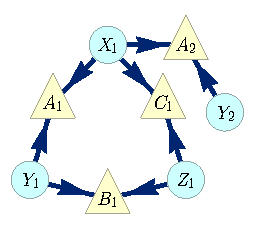
\includegraphics[scale=1]{broadcastingexamplenohighlight.pdf}
\caption{A simple inflation of the Triangle scenario, also notably $\ansubgraph[(\cref{fig:Tri222})]{A_1 A_2 B_1 C_1}$.}\label{fig:simpleinflation}
\end{minipage}\hfill
\begin{minipage}[t]{0.275\linewidth}
\centering
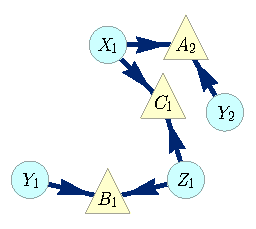
\includegraphics[scale=1]{nobroadcastingexamplenohighlight.pdf}
\caption{An even simpler inflation of the Triangle scenario, also notably $\ansubgraph[(\cref{fig:simpleinflation})]{A_2 B_1 C_1}$. }\label{fig:simplestinflation}
\end{minipage}
\hfill
\begin{minipage}[t]{0.325\linewidth}
\centering
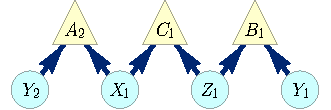
\includegraphics[scale=1]{TriDagSubA2B1C1.pdf}
\caption{Another representation of \cref{fig:simplestinflation}. Despite not containing the original scenario, this is a valid inflation per \cref{eq:definflationDAG}.}\label{fig:TriDagSubA2B1C1}
\end{minipage}
\end{figure}

Let us ask, is it possible for the three original-scenario observable variables $\{A,B,C\}$ to be random but perfectly correlated? We call this the GHZ-type distribution, after an eponymous tripartite entangled quantum state \cite{greenberger1989going,3Qubits2Ways}. So $P_{\text{GHZ}}\parenths{A B C}$ is given by
\begin{align}\label{eq:ghzdistribution1}
p_{\text{GHZ}}\parens{a b c}=\frac{[000]+[111]}{2}=\begin{cases}\tfrac{1}{2}&\text{if }\; a=b=c, \\ 0&\text{otherwise}.\end{cases}
\end{align}
We assume uniform binary variables for the sake of concreteness, but the argument is general. Let's temporarily (falsely) assume $P_{\text{GHZ}}$ to be feasible for the triangle scenario. Since $\brackets{A_2 C_1}$ is an injectable set we have $\pdf{A_2 C_1}=\pdf{A C}$, and therefore $P_{\text{GHZ}}$ implies that $A_2$ and $C_1$ are perfectly correlated. Similarly, since $\brackets{B_1 C_1}$ is an injectable set we have $\pdf{B_1 C_1}=\pdf{A C}$, and therefore $B_1$ and $C_1$ must be perfectly correlated, and by extension $B_1$ and $A_2$ are perfectly correlated as well. On the other hand, $A_2$ and $B_1$ must be statistically independent, as they do not share any common ancestor. The only way for two variables to be \emph{both} perfectly correlated and independent is by being deterministic. This is not the case in $P_{\text{GHZ}}$, and thus we have certified that $P_{\text{GHZ}}$ is not realizable from the Triangle causal structure, recovering the seminal result of \citet{steudel2010ancestors}.

To be clear, one can employ \emph{any} kind of causal infeasibility criteria on the inflation DAGs to constrain the distributions on the original DAG. For example, here's a quantitative version of the same proof against perfect correlation in the Triangle scenario, this time using entropic arguments: Trivially $H(A_2|B_1)\leq H(A_2|C_1)+H(C_1|B_1)$, because the amount of information required to learn $A_2$ from $B_1$ is surely less than the amount of information required to learn  $A_2$ from $C_1$ and also to learn $C_1$ from $B_1$. On the other hand, the marginal independence of $A_2$ and $B_1$ implies $H(A_2|B_1)=H(A_2)$. $P_{\text{GHZ}}$ is ruled out, because it would yield $H(A_2|C_1)=H(C_1|B_1)=0$ while $H(A_2)=1$. The entropic conclusion is $H(A_2)\leq H(A_2|C_1)+H(C_1|B_1)$, or equivalently, $I(A_2:C_1)+I(B_1:C_1)\leq H(C_1)$. The injectability of sets per \cref{fig:TriDagSubA2B1C1} in turn yields
\begin{align}\label{eq:monogomyofcorrelations}
I(A:C)+I(B:C)\leq H(C),
\end{align}
\begin{comment}
\begin{align}
\hspace{-\mathindent}&I(A_2:B_1|C_1)=H(A_2 C_1)+H(B_1 C_1)-H(A_2 B_1 C_1)-H(C_1)\geq 0 
\tag{positivity of conditional MI}\\
\hspace{-\mathindent}\therefore  &H(A_2 C_1)+H(B_1 C_1)-H(A_2 B_1)-H(C_1)\geq 0 
\tag{monotonicity of entropy, $H(A_2 B_1 C_1)\geq H(A_2 B_1)$}\\
\hspace{-\mathindent}\therefore & H(A_2 C_1)+H(B_1 C_1)-H(A_2)-H(B_1)-H(C_1)\geq 0 
\tag{$A_2\bot B_1\implies H(A_2 B_1)=H(A_2)+H(B_1)$}\\
\hspace{-\mathindent}\therefore & H(A_2)+H(B_1)+2H(C_1)-H(A_2 C_1)-H(B_1 C_1)\leq H(C_1)
\tag{rearranging terms}\\
\hspace{-\mathindent}\therefore & I(A_2:C_1)+I(B_1:C_1)\leq H(C_1)
\tag{definition of mutual information}\\
\hspace{-\mathindent}\therefore & I(A:C)+I(B:C)\leq H(C)
\tag{monogamy of correlations}
%\tag{recognition of injectable sets}
\label[]{eq:monogomyofcorrelations}
\end{align}
\end{comment}
an inequality known as monogamy of correlations \cite{fritz2012bell}. It forbids perfect correlation of all three variables. Because \cref{eq:monogomyofcorrelations} is derivable from a non-broadcasting inflation DAG, it follows that monogamy of correlations holds even in the context of generalized probabilistic theories. This recovers a result of \citet[Cor. 24]{pusey2014gdag}. Indeed, Fig. 5 in Ref. \cite{pusey2014gdag} is essentially equivalent to \cref{fig:TriDagSubA2B1C1} here.


\example{: \tred{The W-type distribution cannot arise from the Triangle scenario}}\par\smallskip\nobreak
Another distribution inconsistent with the Triangle scenario is the W-type distribution, named after a quantum state appearing in Ref. \cite{3Qubits2Ways}. To our knowledge, the infeasibility of the Triangle causal structure to explain the W-type distribution is a novel result here. The distribution $P_{\text{W}}\parenths{A B C}$ is given by
\begin{align}\label{eq:wdistribution1}
p_{\text{W}}\parens{a b c}=\frac{[100]+[010]+[001]}{3}=\begin{cases}\tfrac{1}{3}&\text{if }\; a+b+c=1, \\ 0&\text{otherwise}.\end{cases}
\end{align}
To prove that  $P_{\text{W}}$ clashes with the Triangle causal structure, consider the inflation DAG of \cref{fig:Tri222}. The set $\{A_2 C_1\}$ is injectable, so $P_{\text{W}}$ implies that $C_1\eql 0$ whenever $A_2 \eql 1$. Similarly, $B_1\eql 0$ whenever $C_2\eql 1$, and $A_1\eql 0$ whenever $B_2\eql 1$. The independence of $A_2$,$B_2$, and $C_2$ means that $\p{A_2\eql B_2\eql C_2\eql 1}=\nicefrac{1}{8}$ according to $P_{\text{W}}$. But that would imply $\p{A_1\eql B_1\eql C_1\eql 0}\geq\nicefrac{1}{8}$, which contradicts $P_{\text{W}}$, hence $P_{\text{W}}$ cannot arise from the Triangle scenario.

The W-type distribution is difficult to witness as unrealizable using conventional causal inference techniques.
\begin{compactenum}
\item There are no conditional independence relations between the observable nodes of the Triangle scenario. %, so the distribution is observationally Markov with respect to the DAG. 
\item Shannon-type entropic inequalities cannot detect this distribution as not allowed by the Triangle scenario~\cite{fritz2013marginal,chaves2014novel,chaves2014informationinference}. 
\item Moreover, \emph{no} entropic inequality can witness the W-type distribution as unrealizable. \citet{weilenmann2016entropic} have constructed an inner approximation to the entropic cone of the Triangle causal structure, and the W-distribution lies inside this. In other words, a distribution with the same entropic profile as the W-type distribution \emph{can} arise from the Triangle scenario.
\item The newly-developed method of covariance matrix causal inference due to \citet{kela2016covariance}, which gives tighter constraints than entropic inequalities for the Triangle scenario, also cannot detect inconsistency with the W-type distribution.
\end{compactenum}
\par\noindent But the inflation DAG approach can, and does so very easily.


\example{: \tred{The PR-box cannot arise from the Bell scenario}}\par\smallskip\nobreak

\begin{figure}[b]
\centering
\begin{minipage}[t]{0.45\linewidth}
\centering
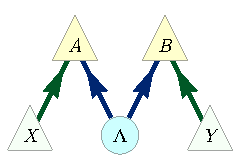
\includegraphics[scale=1]{BellDagRaw.pdf}
\caption{The causal structure of the a bipartite Bell scenario. The local outcomes of Alice's and Bob's experimental probing is assumed to be a function of some latent common cause, in addition to their independent local experimental settings.}\label{fig:NewBellDAG1}
\end{minipage}
\hfill
\begin{minipage}[t]{0.45\linewidth}
\centering
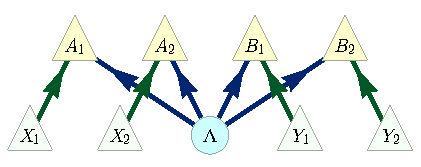
\includegraphics[scale=1]{BellDagCopy.pdf}
\caption{An inflation DAG of the bipartite Bell scenario, where both local settings variables have been duplicated.}\label{fig:BellDagCopy1}
\end{minipage}
\end{figure}

Consider the causal structure associated to the Bell \cite{bell1964einstein,Brunner2013Bell,bell1966lhvm,CHSHOriginal} scenario [\citealp{pusey2014gdag}~(Fig.~E\#2), \citealp{WoodSpekkens}~(Fig.~19), \citealp{chaves2014novel}~(Fig.~1), \citealp{BeyondBellII}~(Fig.~1), \citealp{wolfe2015nonconvexity}~(Fig.~2b), \citealp{steeg2011relaxation}~(Fig.~2)], depicted here in \cref{fig:NewBellDAG1}. The observable variables are $\brackets{A,B,X,Y}$, and $\Lambda$ is the latent common cause of $A$ and $B$. An inflation of the Bell scenario is show in \cref{fig:BellDagCopy1}.

The PR-box distribution is famously inconsistent with the Bell scenario \cite{PROriginal,PRUnit}. Here we prove its unrealizability using inflation DAG logic. The distribution  is given by ${P_{\text{PR}}}\parenths{A B X Y} = P_{\text{PR}}\parenths{A B | X Y} P(X) P(Y)$, where $P(X)$ and $P(Y)$ are arbitrary full-support distributions\footnote{In the literature on the Bell scenario, these variables are known as ``settings''. Generally, We may think of endogenous observable variables as settings, coloring them light green in the DAG figures. Settings variables are natural candidates for conditioning on.} over the binary variables $X$ and $Y$, and
\begin{align}\begin{split}\label{eq:PRbox}
% & p_{\text{PR}}\parens{a b |x y}=\frac{[00|00]+[11|00]+[00|10]+[11|10]+[00|01]+[11|01]+[01|11]+[10|11]}{8}\\
p_{\text{PR}}\parens{a b |x y}=\begin{cases}\tfrac{1}{2}&\text{if }\; \SmallNamedFunction[2]{mod}{a+b}=x\cdot y, \\ 0&\text{otherwise}.\end{cases}
\end{split}\end{align}
We begin by recognizing that $\{A_1 B_1 X_1 Y_1\}$, $\{A_1 B_1 X_2 Y_1\}$, $\{A_1 B_2 X_1 Y_2\}$, and $\{A_2 B_2 X_2 Y_2\}$ are all injectable sets, and that $X_1$, $X_2$, $Y_1$, and $Y_2$ are all independent variables.
% $P_{\text{PR}}$ is given as a conditional distribution because $X$ and $Y$ are settings variables.
No matter how biased the distributions $P(X)$ and $P(Y)$ are, however, surely the event $\{X_1, X_2, Y_1, Y_2\}=\{0, 1, 0, 1\}$ \fxnote{set notation for this?} occurs sometimes. Whenever it does, $P_{\text{PR}}$ specifies perfect correlation between $A_1$ and $B_1$, perfect correlation between $A_1$ and $B_2$, perfect correlation between $A_2$ and $B_1$, and perfect \emph{anti}correlation between $A_2$ and $B_2$. Those four requirements are not mutually compatible: since perfect correlation is transitive, the first three properties entail perfect correlation between $A_2$ and $B_2$. Hence the PR-box distribution is disallowed by the Bell scenario.

%Indeed, this logic rules out much more than just the PR-box: If $\p{A\eql B|X\eql Y\eql 1}=0$ then we can quickly derive a Hardy-type argument.
%\begin{align}\begin{split}
%&\p{A_1\eql B_1|X_1\eql Y_1\eql 0}=\textstyle{\sum\nolimits_q} \p{A_1\eql B_1\eql q|X_1\eql Y_1\eql 0}\\
%&=\textstyle{\sum\nolimits_q} \p{A_1\eql B_1\eql q|X_1\eql Y_1\eql 0,X_2\eql Y_2\eql 1}\qquad\left(\text{because }A_1 B_1 \bot X_2 Y_2 | X_1 Y_1\right)\\
%&=\textstyle{\sum\nolimits_q} \p{A_1\eql B_1\eql A_2\eql q|X_1\eql Y_1\eql 0,X_2\eql Y_2\eql 1}+\p{A_1\eql B_1\eql q,A_2\cramp{\neq} q|X_1\eql Y_1\eql 0,X_2\eql Y_2\eql 1}\\
%&=\textstyle{\sum\nolimits_q} \p{A_1\eql B_1\eql q, B_2\cramp{\neq} q|X_1\eql Y_1\eql 0,X_2\eql Y_2\eql 1}+\p{A_1\eql B_1\eql q,A_2\cramp{\neq} q|X_1\eql Y_1\eql 0,X_2\eql Y_2\eql 1}\\
%&\qquad\left(\text{because }A_2\eql q |X_2\eql Y_2\eql 1 \Leftrightarrow B_2\cramp{\neq} q |X_2\eql Y_2\eql 1\right)\\
%&\leq\textstyle{\sum\nolimits_q}\p{A_1\eql q, B_2\cramp{\neq} q|X_1\eql Y_1\eql 0,X_2\eql Y_2\eql 1}+\p{B_1\eql q,A_2\cramp{\neq} q|X_1\eql Y_1\eql 0,X_2\eql Y_2\eql 1}\\
%&=\textstyle{\sum\nolimits_q} \p{A_1\eql q, B_2\cramp{\neq} q|X_1\eql 0, Y_2\eql 1}+\p{B_1\eql q,A_2\cramp{\neq} q| Y_1\eql 0,X_2\eql 1}\\
%&= \p{A_1\cramp{\neq}B_2|X_1\eql 0, Y_2\eql 1}+\p{A_2\cramp{\neq}B_1| Y_1\eql 0,X_2\eql 1}\\
%&\therefore \p{A=B|X\eql Y\eql 0}\leq \p{A\neq B|X\eql 1,Y\eql 0}+\p{A\neq B|X\eql 0,Y\eql 1}
%\end{split}\end{align}

\begin{comment}
\example{: \tred{The center-break distribution cannot arise from the Instrumental scenario}}\par\smallskip\nobreak
\begin{figure}[t]
\centering
\begin{minipage}[b]{0.375\linewidth}
\centering
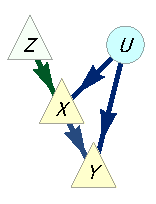
\includegraphics[scale=1]{InstrumentalDAGpearl.pdf}
\caption{The Instrumental scenario}\label{fig:instrumental}
\end{minipage}\hspace{80pt}
\begin{minipage}[b]{0.4\linewidth}
\centering
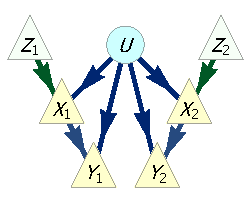
\includegraphics[scale=1]{InstrumentalInflation.pdf}
\caption{An inflation of the Instrumental scenario.}\label{fig:instrumentalinflation}
\end{minipage}\hfill
\end{figure}

The (disallowed) center-break distribution for the Instrumental scenario is one in which $Y$ and $Z$ are perfectly correlated while $X$ is fixed as a point distribution, i.e. returning one outcome with 100\% probability.
\begin{align}\begin{split}\label{eq:PRbox}
&{P_{\text{CB}}}\parenths{X Y Z} \coloneqq\quad p_{\text{CB}}\parens{x y z} y}=\frac{[000]+[011]}{2}=\begin{cases}\tfrac{1}{2}&\text{if }\; y\eql z \land x\eql0 \\ 0&\text{otherwise}\end{cases}
\end{split}\end{align}
We prove its infeasibility by considering the inflation DAG in \cref{fig:instrumentalinflation}. 
\end{comment}


The following section discusses how to procedurally derive polynomial infeasibility criteria pertaining to original DAG from properties of an inflation DAG. 



\begin{comment}\btob
The basic idea of our method is disarmingly simple, so let us illustrate it first with an example before presenting the general case in more formal detail. Consider the W-type distribution on the Triangle scenario,
\[	p(001) = p(010) = p(100) = \frac{1}{3}.\]
So our question is, can this distribution over $A$, $B$ and $C$ be obtained through the causal structure of~\cref{fig:TriMainDAG}? For the sake of the argument, assume that this is the case; hence there are distributions over the hidden variables $p(X)$, $p(Y)$ and $p(Z)$ as well as conditional distributions $p(A|X,Y)$, $p(B|Y,Z)$ and $p(C|X,Z)$ such that $p(ABC)$ is reproduced. Intuitively, we may think of $X$ as a ``black box'' system that outputs random stuff, and likewise of $A$ as a black box which takes some inputs and outputs random signals. Now there are two things that we can do in order to 
\begin{itemize}
\item Of each outgoing variable we can produce an arbitrary number of further copies, resulting in new edges;
\item Of each black box, we can likewise produce copies that behave independently, resulting in new nodes.
\end{itemize}
We can then rewire these gadgets into a new Bayesian network.~\cref{fig:TriFullDouble} presents an example of such a rewiring, or ``inflated'' DAG. Pearl's \emph{do calculus} uses rewirings of a similar nature, and also Henson, Lal and Pusey~\cite{pusey2014gdag} use this reasoning to show that the entropic inequality $I(A:B) + I(B:C)\leq H(B)$ holds in all GPTs, just without taking copies of variables but only rewiring the boxes.

Since the outcome $B=1$ occurs sometimes, there must be hidden variables values $a_2$ and $c_3$ such that $B_4=1$ has positive probability; and similarly, we choose values for $X_1$ and $Y_1$ such that $A_1=1$ has positive probability, and for $X_2$ and $Z_1$ such that $C_2=1$ has positive probability. Since all the hidden variables in the inflated DAG are independent, these conditions do sometimes all occur jointly. Then by the form of the assumed distribution, it follows that for the assumed values of the hidden variables, one must necessarily have $A_2=0$, $B_3=0$ and $C_1=0$, which contradicts the assumption $p(000) = 0$.

It is not difficult to transform this argument into a polynomial inequality for the Triangle scenario. However, it is more instructive to present the derivation of polynomial inequalities using our method in a slightly different manner, and we will do so later.
\etob\end{comment}


\section{A procedure for deriving polynomial inequalities}
\label{sec:ineqs}

%\purp{NEW PLAN (As of Sunday): Main text gets marginal's problem explanation, appendix get full nonlinear treatment.} 

Our final goal in deriving polynomial inequalities is to derive constraints on the distribution of the observable variables in the original DAG. We accomplish this by proxy, namely by deriving constraints on the distributions over the variables in the pre-injectable sets of the inflation DAG. Just as distributions over the pre-injectable sets translate into distributions pertaining to the original DAG variables per \cref{eq:coincidingdistrodef}, so do \emph{constraints} on the distributions of pre-injectable sets translate into constraints on the original DAG variables.

We are aware of a variety of methods for identifying interesting constraints on the distributions over the variables in the pre-injectable sets. But here, we focus on the very simplest and weakest such constraint: the nonnegativity of probabilities together with the factorization~\cref{eq:preinjfactor}. In fact, this is all that we have used in the previous section as well.

Our method is based on deriving inequalities for the so-called \tblue{marginal problem}. This relies on linear quantifier elimination, which is computationally feasible in at least some cases. A nonlinear method for deriving even tighter constraints is discussed in appendix \cref{sec:nonlinearelimination}. The simpler method discussed here consists of two steps: 1) Identify the pre-injectable sets, and 2) Solve the marginal problem with respect to the pre-injectable sets.


\step{: \tred{Identifying the Pre-Injectable Sets}}\label{step:findpreinjectable}\par\smallskip\nobreak

To identify the pre-injectable sets, we first identify the injectable sets. To this end, it is useful to construct an auxiliary graph from the inflation DAG. Let the nodes of these auxiliary graphs be the observable nodes in the inflation DAG. The \tblue{injection graph}, then, is the undirected graph in which a pair of nodes $A_i$ and $B_j$ are adjacent if  $\An{A_i B_j}$ is irredundant. The injectable sets are then precisely the cliques\footnote{A clique is a set of nodes such that every single node is connected to every other.} in this graph, per \cref{eq:definjectable2}. 

Determining the pre-injectable sets from there can be done via constructing another graph that we call the \tblue{independence graph}. Its nodes are the injectable sets, and we connect two of these by an edge if their ancestral subgraphs are disjoint. Then by definition, the pre-injectable sets can be obtained as the cliques in this graph. Taking the union of all the injectable sets in such a clique results in a pre-injectable set. Since it is sufficient to only consider the maximal pre-injectable sets, one can eliminate all those pre-injectable sets that are contained in other ones, as a final step.

Let us also define the \tblue{ancestral dependence graph}, in which two nodes are adjacent if they share a common ancestor, and its complement the \tblue{ancestral independence graph}, in the ancestrally independent nodes are adjacent. To ascertain the factorization of a node set $\bm{U}$ into ancestrally-independent partitions one considers the subgraph on  $\bm{U}$ of the ancestral dependence graph: the ancestrally-independent partitions are identically the distinct connected components of that subgraph. By examining the injection graph and the ancestral dependence graph, therefore, one is able to quickly determine all injectable sets and all ancestral independence relations.

%It is also useful to define another auxiliary graph, the \tblue{pre-injection graph} in which a pair of nodes $A_i$ and $B_j$ are connected if either $\An{A_i B_j}$ or if $A_i\aindep B_j$. The pre-injection graph is identically the union of the injection graph with the ancestral independence graph. Any clique in the pre-injection graph is \emph{not} necessarily a pre-injectable set, but every pre-injectable set must correspond to a clique in the pre-injection graph, per \cref{eq:defpreinjectable}. Moreover, maximal-size pre-injectable sets must correspond to maximal cliques in the pre-injection graph. This makes the pre-injection graph a handy tool for determining the pre-injectable sets. We start by enumerating all maximal cliques in the pre-injection graph to obtain candidate pre-injectable sets. Each candidate set is then factored into ancestrally-independent partitions by means of the ancestral dependence graph. A candidate set is a legitimately pre-injectable if and only if all of its ancestrally-independent partitions are themselves injectable. Isolating the genuine pre-injectable sets from the candidates is therefore quite easy, especially since the complete set of injectable sets is already known.

\begin{figure}[t]
\centering
\begin{minipage}[b]{0.3\linewidth}
\centering
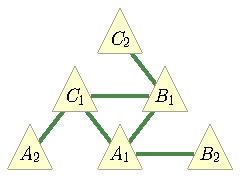
\includegraphics[scale=1]{injectiongraph222.pdf}
\caption{The auxiliary injection graph corresponding to the inflation DAG in \cref{fig:Tri222}, wherein a pair of nodes are adjacent iff they are pairwise injectable.}\label{fig:injection222}
\end{minipage}
\hfill
\begin{minipage}[b]{0.3\linewidth}
\centering
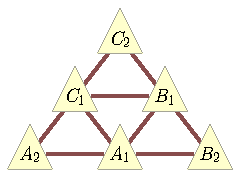
\includegraphics[scale=1]{ancestraldependancegraph222.pdf}
\caption{An auxiliary ancestral dependance graph corresponding to the inflation DAG in \cref{fig:Tri222}, wherein a pair of nodes are adjacent iff they share a common ancestor.}\label{fig:dependances222}
\end{minipage}
\hfill
\begin{minipage}[b]{0.3\linewidth}
\centering
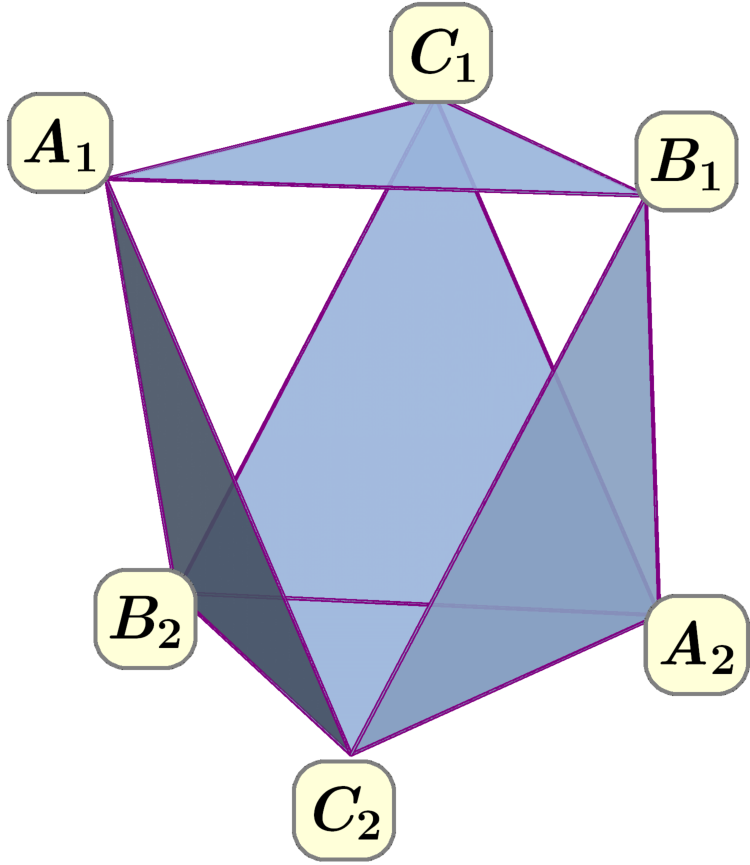
\includegraphics[scale=0.2]{simplicialcomplex.pdf}
\caption{The simplicial complex... \purp{Tobias - you please caption this?}The 5 faces in this figure correspond to the pre-injectable sets.}\label{fig:simplicialcomplex222}
\end{minipage}
\end{figure}

Applying these prescriptions to the inflation DAG in \cref{fig:Tri222} identifies the following 
 ancestral independences 
maximal injectable and maximal pre-injectable sets as follows:
\begin{align}\label{eq:basicsetup222}
{\underbrace{\begin{matrix}
A_2\aindep B_1\\
A_2\aindep C_2\\
B_2\aindep A_2\\
B_2\aindep C_1\\
C_2\aindep A_1\\
C_2\aindep B_2
\end{matrix}}_{\substack{\text{pairwise}\\\text{ancestral}\\\text{independences}}}}
\qquad\quad
{\underbrace{\begin{matrix}
\\ \\
\brackets{A_2}\aindep \brackets{B_1 B_2 C_2}\\
\brackets{B_2}\aindep \brackets{A_2 C_1 C_2}\\
\brackets{C_2}\aindep \brackets{A_1 A_2 B_2}\\
\brackets{A_2}\aindep \brackets{B_2}\aindep \brackets{C_2}
\end{matrix}}_{\substack{\text{maximal}\\\text{ancestral}\\\text{independences}}}}
\qquad\quad
{\underbrace{\begin{matrix}
\brackets{ A_1 B_1 }\\
\brackets{ B_1 C_1 }\\
\brackets{ A_1 C_1 }\\
\brackets{ A_2 C_1 }\\
\brackets{ B_2 A_1 }\\
\brackets{ C_2 B_1 }\\
\end{matrix}}_{\substack{\text{pairwise}\\\text{injectable}\\\text{sets}}}}
\qquad\quad
{\underbrace{\begin{array}{l}
\\ \\
\brackets{A_1 B_2}\\
\brackets{B_1 C_2}\\
\brackets{A_2 C_1}\\
\brackets{A_1 B_1 C_1}
\end{array}}_{\substack{\text{maximal}\\\text{injectable}\\\text{sets}}}}
\qquad\quad
{\underbrace{\begin{matrix}
\\
\brackets{A_1 B_1 C_1} \\
\brackets{A_1 B_2 C_2} \\
\brackets{A_2 B_1 C_2} \\
\brackets{A_2 B_2 C_1} \\
\brackets{A_2 B_2 C_2}
\end{matrix}}_{\substack{\text{maximal}\\\text{pre-injectable}\\\text{sets}}}}
\end{align}
such that the distributions on the pre-injectable sets relate to the original DAG distribution via
\begin{align}\label{eq:preinjectableuses222}
\begin{split}
&\pdf{A_1 B_1 C_1} = \pdf{A B C} \\
&\pdf{A_1 B_2 C_2} = \pdf{C}\pdf{A B}\\
&\pdf{A_2 B_1 C_2} = \pdf{A}\pdf{B C}\\
&\pdf{A_2 B_2 C_1} = \pdf{B}\pdf{A C}\\
&\pdf{A_2 B_2 C_2} = \pdf{A}\pdf{B}\pdf{C}
\end{split}
\end{align}
Having identified the pre-injectable sets (and how to use them), we next turn to deriving constraints on the distributions over the pre-injectable sets.


\step{: \tred{Constraining the Distribution over Pre-Injectable Sets via the Marginal Problem}}\label{step:marginalsproblem}\par\smallskip\nobreak

The most trivial constraint possible 
%on the pre-injectable set
is the \emph{existence of a joint probability distribution} over all the observable variables in the inflation DAG. Each of the five three-variable distributions in \cref{eq:preinjectableuses222} is a different marginal distribution of the six-variable joint distribution $\pdf{A_1 A_2 B_1 B_2 C_1 C_2}$. Solving the marginal problem means finding inequalities on the marginal distributions such that the inequalities will satisfied only if there exists some joint distribution from which the distributions on the marginal sets can be recovered through marginalization. The marginal problem comes up in a variety of applications, and has been studied extensively; see~\cite{fritz2013marginal} for further references.\purp{Tobias, say better? And add citations please!} \purp{T: Ok, I'll get back to this on my second iteration} 

\purp{Comment about how solving marginals problem still gives polynomial inequalities.}

From now on, one can apply \emph{any} method for dealing with the marginal problem. For example if one is given a particular distribution $P$ over the original scenario variables, then one can use~\cref{eq:preinjfactor} to compute the marginal distributions over the pre-injectable sets in an inflation DAG. Efficient linear programming can be used to to check whether there exists a joint distribution reproducing these marginals \cite{Korovin2012ImplementingCRA,Bobot2012SimplexSAT}. If such a joint distribution does not exist, then the given original-scenario distribution is witnessed as inconsistent with the original causal structure. If a joint distribution \emph{does} exist then the problem remains open, and one can try again using a different inflation.

In order to derive inequalities that hold for \emph{all} distributions that are feasible on the original DAG, say for a given number of outcomes per variable, we can formally solve the marginal problem via linear quantifier elimination, as we review in the following. This consists of eliminating unknowns from a set of linear inequalities and equalities.

The linear inequalities correspond to the nonnegativity of the joint distribution. Formally, the probability of any possible assignment of outcomes to to the observable variables is constrained to be nonnegative. For the six observable variables in \cref{fig:Tri222}, for example, the linear inequalities are given by $0\leq \pdf{A_1 A_2 B_1 B_2 C_1 C_2}$. Note than a single inequality (or equality) pertaining to a probability \emph{distribution} is actually shorthand for a whole set of inequalities (or equalities) pertaining to the probabilities of individual events. Taking the observable variables to be binary, for example, would mean that $0\leq \pdf{A_1 A_2 B_1 B_2 C_1 C_2}$ would be shorthand for 64 distinct nonnegativity inequalities, namely
\begin{align}\label[eqs]{eq:nonnegativities}
\begin{split}
 & 0\leq \p{a_1 a_2 b_1 b_2 c_1 c_2} ,\quad
 0\leq \p{\n{a}_1 a_2 b_1 b_2 c_1 c_2} ,\quad
 0\leq \p{a_1 \n{a}_2 b_1 b_2 c_1 c_2} ,\quad...\quad,\\
 &
 0\leq \p{\n{a}_1 \n{a}_2 b_1 b_2 c_1 c_2} ,\quad
 0\leq \p{\n{a}_1 a_2 \n{b}_1 b_2 c_1 c_2}, \quad ...
\end{split}
\end{align}
etc. For a marginals problem based on the joint existence of $n$ observable variables, each ranging over $r$ possible outcomes, one would initialize the problem with $r^n$ linear nonnegativity inequalities. Unlike probabilities pertaining to injectable sets, these joint probabilities are \emph{not} fully specified by probabilities which are observed in the original scenario. We coin the term \tblue{gedankenprobability} to denote a probability pertaining to a not-pre-injectable set of inflation-DAG variables. The gedankenprobabilities evoke thought experiments, because knowing the original-scenario causal model determines the gedankenprobabilities. % \emph{in-principle}.

The linear equations in the marginal problem are those equations which express each of the marginal probabilities as a sum over various different gedankenprobabilities, namely marginalization. Again using distribution shorthand, the five marginal distributions in \cref{eq:preinjectableuses222} would correspond to the equations
\begin{align}\label[eqs]{eq:marginalequalities222}
\begin{split}
&\pdf{A_1 B_1 C_1} = \sum\nolimits_{A_2 B_2 C_2}\pdf{A_1 A_2 B_1 B_2 C_1 C_2},\\
&\pdf{A_1 B_2 C_2} = \sum\nolimits_{A_2 B_1 C_1}\pdf{A_1 A_2 B_1 B_2 C_1 C_2},\\
&\pdf{A_2 B_1 C_2} = \sum\nolimits_{A_1 B_2 C_1}\pdf{A_1 A_2 B_1 B_2 C_1 C_2},\\
&\pdf{A_2 B_2 C_1} = \sum\nolimits_{A_1 B_1 C_2}\pdf{A_1 A_2 B_1 B_2 C_1 C_2},\\
&\pdf{A_2 B_2 C_2} = \sum\nolimits_{A_1 B_1 C_1}\pdf{A_1 A_2 B_1 B_2 C_1 C_2}.
\end{split}
\end{align}
To be clear, taking the observable variables to be binary would mean that each equality in \cref{eq:marginalequalities222} is shorthand for 8 distinct marginalization equations. For example the equality $\pdf{A_1 B_1 C_1} = \sum\limits_{A_2 B_2 C_2}\pdf{A_1 A_2 B_1 B_2 C_1 C_2}$ is shorthand for 8 equations of the form
\begin{align}
\p{A_1\eql a,  B_1\eql b, C_2\eql c} = \sum\limits_{a' b' c'}\p{a_1 {a'}_2 {b}_1 {b'}_2 {c}_1 {c'}_2}
\end{align}
for each of the 8 possible values of the tuple $\{a b c\}$.

Solving the marginal problem means eliminating all the gedankenprobabilities such as $\p{a_1 {a'}_2 {b}_1 {b'}_2 {c}_1 {c'}_2}$ from the system of inequalities and equalities. Practically, this is accomplished by linear quantifier elimination. As an equivalent description of the same problem, but could likewise consider the problem of determining the facets of the marginal polytope, the vertices of which are known to be given by the deterministic points (compare Fine's theorem~\cite{FineTheorem} in the Bell scenario case).

Geometrically, linear quantifier elimination is equivalent to projecting a high-dimensional polytope in halfspace representation (inequalities and equalities) into a lower-dimensional quotient space.

Polytope projection is a well-understood problem in computational optimization, and a surprising variety of algorithms are available for the task \cite{jones2004equality,JonesThesis2005,Jones2008}. The oldest-known method for polytope projection, i.e. linear quantifier elimination, is an algorithm known as Fourier-Motzkin (FM) elimination \cite{fordan1999projection,DantzigEaves}, although Fourier-Cernikov elimination variant \cite{Shapot2012,Bastrakov2015}, as well as Block Elimination and Vertex Enumeration \cite{Avis2000lrs}, are also fairly popular. More advanced polytope projection algorithms, such as Equality Set Projection (ESP) and Parametric Linear Programming, have also recently become available \cite{jones2004equality,JonesThesis2005,Jones2008}. 

Linear quantifier elimination routines are available in many software tools\footnote{For example \textit{MATLAB$^{_{\textit{\tiny\texttrademark}}}$}'s \href[pdfnewwindow]{http://people.ee.ethz.ch/~mpt/2/docs/refguide/mpt/@polytope/projection.html}{\texttt{MPT2}}/\href[pdfnewwindow]{http://ellipsoids.googlecode.com/svn-history/r2740/branches/issue_119_vrozova/tbxmanager/toolboxes/mpt/3.0.14/all/mpt3-3_0_14/mpt/modules/geometry/sets/@Polyhedron/projection.m}{\texttt{MPT3}}, \textit{Maxima}'s \href[pdfnewwindow]{http://maxima.sourceforge.net/docs/manual/de/maxima_75.html}{\texttt{fourier\_elim}}, \textit{lrs}'s \href[pdfnewwindow]{http://cgm.cs.mcgill.ca/~avis/C/lrslib/USERGUIDE.html\#fourier}{\texttt{fourier}}, or \textit{Maple$^{_{\textit{\tiny\texttrademark}}}$}'s (v17+) \href[pdfnewwindow]{http://www.maplesoft.com/support/help/maple/view.aspx?path=RegularChains/SemiAlgebraicSetTools/LinearSolve}{\texttt{LinearSolve}} and \href[pdfnewwindow]{http://www.maplesoft.com/support/help/Maple/view.aspx?path=RegularChains/SemiAlgebraicSetTools/Projection}{\texttt{Projection}}. The efficiency of most of these software tools, however, drops off markedly when the dimension of the final projection is much smaller than the initial space of the inequalities. FM elimination aided by Cernikov rules \cite{Shapot2012,Bastrakov2015} is implemented in \href[pdfnewwindow]{http://sbastrakov.github.io/qskeleton/}{\textit{qskeleton}} \cite{qskeleton}. ESP  \cite{jones2004equality,JonesThesis2005,Jones2008} is supported by \href[pdfnewwindow]{http://people.ee.ethz.ch/~mpt/2/docs/refguide/mpt/@polytope/projection.html}{\texttt{MPT2}} but not \href[pdfnewwindow]{http://people.ee.ethz.ch/~mpt/3/}{\texttt{MPT3}}, and by the (undocumented) option of \href[pdfnewwindow]{https://github.com/tulip-control/polytope/blob/master/polytope/polytope.py\#L1406}{projection} in the \href[pdfnewwindow]{https://pypi.python.org/pypi/polytope}{\textit{polytope}} (v0.1.1 2015-10-26) python module.}. We have found custom-coding an linear elimination routine in \textit{Mathematica$^{_{\textit{\tiny\texttrademark}}}$} to be most efficient, see \cref{sec:projalgorithms} for further detail.
%\footnote{FM elimination algorithms make intermittent calls to a linear-programming subroutine for eliminating redundant inequalities. The authors found an efficient implementation of this subroutine in \textit{Mathematica$^{_{\textit{\tiny\texttrademark}}}$}, see \cref{sec:redundancy} for further details.}.
%Fourier-Motzkin elimination appreciable suboptimal, however, when the dimension of the final projection is much smaller than the initial space of the inequalities, i.e. when there are many gedankenprobabilities. See Refs. \cite{jones2004equality,JonesThesis2005,Jones2008} and \cref{sec:projalgorithms} for further detail.


Linear quantifier elimination is already widely used in causal inference to derive entropic inequalities \cite{fritz2013marginal,chaves2014novel,chaves2014informationinference}. In that task, however, the quantifiers being eliminated are those entropies which refer to hidden variables. By contrast, the probabilities we consider here are exclusively in terms of observable variables right from the very start. The quantifiers we eliminate are the gedankenprobabilities, which are quite different from probabilities involving hidden variables.

Although linear quantifier elimination can be highly optimized, it can still prove computationally difficult. It is therefore sometimes useful to consider relaxations of the marginals problem. The \emph{full} marginals problem is to find inequalities on the marginal distributions such that the inequalities are satisfied \emph{if and only if} the given marginal distributions can be extended. It is much easier to generate necessary-but-insufficient inequalities, i.e. satisfied by all compatible marginal distributions but such that no-violation does not certify compatibility. We have identified a technique for rapidly generating such quantifier-free inequalities by restricting the search to inequalities of a very particular form. We found this alternative technique — trading generality for speed — to be extraordinarily practical. The type of inequalities that we consider are given by a certain class of tautologies in classical propositional logic, see \cref{sec:TSEM} for further details.

%One useful alternative to linear quantifier elimination is to identify representative probability distributions which are incompatible with the (unprojected) constraints; \citet{ChavesNoSignalling} use this technique, for example. %That technique essentially translates the elimination problem to a satisfiability problem, and moreover an ultra-efficient \emph{linear} quantifier existence problem at that! In the context of polytope projection, these representative probability distributions correspond to extreme rays of the so-called ``projection cone" \cite{jones2004equality,Jones2008,BalasProjectionCone}.

%A final alternative to linear quantifier elimination is to restrict one's consideration to quantifier-free inequalities with a particular form. We found this alternative technique — trading generality for speed — to be extraordinarily practical. The subtype of causal criteria which can be most rapidly recognized are those which follow from certain tautologies in classical propositional logic, see \cref{sec:TSEM} for further details.




%\purp{It is interesting to compare the technique for deriving polynomial inequalities here to that in in Ref. \cite{ChavesPolynomial}. One the one hand, our initial set of linear inequalities is much stronger, as we work with the inflated DAG whereas \citet{ChavesPolynomial} considers only the original DAG. This allows us to analyze scenarios which Ref. \cite{ChavesPolynomial} cannot, namely those without any observable conditional independence relations, such as the Triangle scenario. On the other hand, Ref. \cite{ChavesPolynomial} purportedly incorporates any kind of observable conditional independence relation, whereas we account only for \emph{unconditional} independence relations, per \cref{step:fac}. A careful examination of Ref. \cite{ChavesPolynomial}, however, reveals that only unconditional independence relations are utilized in all the example there. To that extent, therefore, all the explicit results in Ref. \cite{ChavesPolynomial} are implied by the inflation DAG technique.}

%We note that our polynomial inequalities are related to those introduced recently by \citet{ChavesPolynomial}, in that our inequalities subsume the explicit results of Ref. \cite{ChavesPolynomial}. \purp{NEEDS CONFIRMATION!} \citet{ChavesPolynomial} exploits conditional independence at the observable level only, whereas our technique is applicable to scenarios even without any observable CI relations, such as the Triangle scenario.


As far as we can tell, our inequalities are not related to the nonlinear infeasibility criteria which have been derived specifically to constrain classical networks \cite{TavakoliStarNetworks,RossetNetworks,TavakoliNoncyclicNetworks}, nor to the nonlinear inequalities which account for interventions to a given causal structure \cite{kang2007polynomialconstraints,steeg2011relaxation}.

\section{Examples of Polynomial Inequalities for the Triangle Scenario}\label{sec:examplebaddistributions}

\purp{T: why not just refer to the list of ineqs here, state that we've done a successful quantifier elimination to demonstrate its practicality, and discuss one or two of the most interesting ineqs?}

Here are some examples of causal infeasibility criteria for the Triangle scenario which we can derive by considering inflation DAGs.

The nontrivial polynomial inequality 
\begin{align}\label{eq:tritrivial1}
{\p{a} + \p{b} + \p{c}} \leq {1 + \p{a} \p{b} + \p{a c} + \p{b c}}
\end{align}
is found to be a constraint on the Triangle scenario through by summing the follow two inequalities
\begin{align}\begin{split}\label{eq:trisimplestunmapped}
 &0\leq  1 -\p{a_2} - \p{b_1} - \p{c_1}+ \p{a_2 b_1} + \p{a_2 c_1} + \p{b_1 c_1}  -\p{a_2 b_1 c_1} \quad\left[=\p{\n{a}_2 \n{b}_1 \n{c}_1}\right]
\\&0\leq \p{a_2 b_1 c_1}
\end{split}\\
\shortintertext{subject to the following transformations}
&  \underbrace{\larray{\\\p{a_2 b_1} \to \p{a_2} \p{b_1}}}_{\text{Factorization relation, per \cref{eq:dfac222}.}} \quad \text{and}\qquad
 \underbrace{\begin{array}{c}
 \p{a_2}\to\p{a}\,, 
\; \p{b_1}\to\p{b}\,, 
\; \p{c_1}\to\p{c},
\\ \p{a_2 c_1}\to \p{a c},
\; \p{b_1 c_1}\to \p{b c}
\end{array}}_{\text{Mapping relations, per \cref{eq:map222}}}.
\end{align}
Indeed, this example has been chosen because \cref{eq:tritrivial1} can be derived directly from the small ancestral subgraph of $\{A_2 B_1 C_1\}$, namely \cref{fig:TriDagSubA2B1C1}.

It may be constructive to rewrite this inequality in correlator form using outcomes in $\{-1,+1\}$ as
\[
	\langle AC\rangle - \langle BC\rangle \leq 1 - \langle A\rangle\langle B\rangle,
\]
which indicates that like~\cref{eq:monogomyofcorrelations}, it is also a sort of monogamy inequality: it is impossible for $A$ and $C$ to be strongly correlated while $B$ and $C$ are strongly anticorrelated.

A consequence of \cref{eq:tritrivial1} is that the perfect correlation distribution per \cref{eq:ghzdistribution1} 
%\begin{align}\label{eq:ghzdistribution}
%{P_{\text{GHZ}}}\parenths{A B C} \coloneqq\quad p_{\text{GHZ}}\parens{a b c}=\frac{[000]+[111]}{2}=\begin{cases}\tfrac{1}{2}&\text{if }\; a=b=c \\ 0&\text{otherwise}\end{cases}
%\end{align}
is found to be unrealizable from the Triangle scenario. This conclusions follows by considering the special case of \cref{eq:tritrivial1} where $a\cramp{\to}1$, $b\cramp{\to}1$, $c\cramp{\to}0$.
%To see how this distribution is incompatible with \cref{eq:tritrivial1}, note that for three \emph{identically distributed} (but not independent) binary variables a further special case of \cref{eq:tritrivial1} is
%\begin{align*}\begin{split}
%&\hspace{-6ex}3\p{A\cramp{=}1}\leq 1+\p{A\cramp{=}1}^2+2\p{A\cramp{=}B\cramp{=}1}.
%\end{split}\end{align*}
%For the W-distribution ${\p{A\cramp{=}B\cramp{=}C\cramp{=}0}=0}$, and also ${\p{A\cramp{=}1,B\cramp{=}1}=0}$, yet ${\p{A\cramp{=}1}=\nicefrac{1}{3}}$. As ${(\nicefrac{1}{3})^3\nleq 0}$ we have proven that the W-type distribution is incompatible with the Triangle scenario.
%Earlier works have already shown that the GHZ-type distribution is incompatible with the classical Triangle scenario \cite{steudel2010ancestors,fritz2012bell,chaves2014novel}. Interestingly, however, the entropic monogamy relation $I\parens{A:B}+I\parens{A:C}\leq H\parens{A}$ which rejects the GHZ-type distribution has been shown also to hold if the hidden shared resources are non-classical, even using generalized probabilistic theories \cite[Cor. 24]{pusey2014gdag}. 


\bigskip
Slightly more involved but otherwise analogous considerations give rise to the inequality
\begin{align}\label{eq:trifancyunmapped}
  &  \p{a_2 b_2 c_2}\leq {\p{\n{a}_1 \n{b}_1 \n{c}_1} + \p{a_1 b_2 c_2} + \p{a_2 b_1 c_2} + \p{a_2 b_2 c_1}} \\
\shortintertext{which in turn yields}
\label{eq:FritzF3}
  & \p{a} \p{b} \p{c} \leq {\p{\n{a} \n{b} \n{c}} +\p{c}\p{a b}  + \p{b}\p{a c}  + \p{a} \p{b c}}\\
\shortintertext{per}
&\qquad
 \underbrace{\begin{array}{l}
 \p{a_1 b_2 c_2}\to \p{c_2} \p{a_1 b_2} \\
 \p{a_2 b_1 c_2}\to \p{a_2} \p{b_1 c_2} \\
 \p{a_2 b_2 c_1}\to \p{b_2} \p{a_2 c_1} \\
 \p{a_2 b_2 c_2}\to \p{a_2} \p{b_2} \p{c_2} \\
\end{array}}_{\text{Factorization relations}}   \quad \text{ and }\quad
\underbrace{\begin{array}{l}
\p{a_1 b_2} \to \p{a b} \\
\p{a_2 c_1} \to \p{a c} \\
\p{b_1 c_2} \to \p{b c} \\
\p{\n{a}_1 \n{b}_1 \n{c}_1}\to \p{\n{a} \n{b} \n{c}}  \\
\end{array}\,.}_{\text{Nontrivial mapping relations}}
\end{align}
A consequence of \cref{eq:FritzF3} is that the W-type distribution per \cref{eq:wdistribution1}
%\begin{align}\label{eq:wdistribution}
%{P_{\text{W}}}\parenths{A B C} \coloneqq\quad p_{\text{W}}\parens{a b c}=\frac{[100]+[010]+[001]}{3}=\begin{cases}\tfrac{1}{3}&\text{if }\; a+b+c=1 \\ 0&\text{otherwise}\end{cases}
%\end{align}
is found to be unrealizable from the Triangle scenario, by considering the special case of \cref{eq:FritzF3} where $a\cramp{\to}1$, $b\cramp{\to}1$, $c\cramp{\to}1$. \cref{eq:FritzF3} requires the use of a broadcasting inflation, and therefore does not hold in the context of general probability theories.

%, where $a,b,c\in\brackets{0,1}$.
%The W-distribution states that the in any event in which $A,B,C$ are observed, precisely one of them will be found to equal $1$ while the other two will equal $0$. The identity of the variable which takes the value $1$ is uniformly random. In informal but intuitive notation, the W-type distribution is ${\nicefrac{1}{3}[100]+\nicefrac{1}{3}[010]+\nicefrac{1}{3}[001]}$.
%To see how this distribution is incompatible with \cref{eq:FritzF3}, note that for three \emph{identically distributed} (but not independent) binary variables a further special case of \cref{eq:FritzF3} is
%\begin{align*}\begin{split}
%&\hspace{-6ex}\p{A\cramp{=}1}^3\leq \p{A\cramp{=}B\cramp{=}C\cramp{=}0} + 3\times\p{A\cramp{=}B\cramp{=}1}\p{C\cramp{=}1}.
%\end{split}\end{align*}
%For the W-distribution ${\p{A\cramp{=}B\cramp{=}C\cramp{=}0}=0}$, and also ${\p{A\cramp{=}1,B\cramp{=}1}=0}$, yet ${\p{A\cramp{=}1}=\nicefrac{1}{3}}$. As ${(\nicefrac{1}{3})^3\nleq 0}$ we have proven that the W-type distribution is incompatible with the Triangle scenario.


\begin{comment}
\section{Failure of Entropic Inequalities}\label{sec:entropiccontrast}

It is interesting to note that entropic inequalities \cite{fritz2013marginal,chaves2014novel,chaves2014informationinference} fail to detect the unrealizability of the W-type distribution [\cref{eq:wdistribution1}] with respect to the Triangle scenario [\cref{fig:TriMainDAG}].
The polynomial inequality (\ref{eq:FritzF3}), by contrast, is a better causal infeasibility criterion in that it successfully rejects the W-type distribution. 

The entropic inequalities associated with the Triangle scenario are given by 
\begin{align}\label{eq:entropicineqs}\begin{split}
&I\parens{A:B}+I\parens{A:C}\leq H\parens{A}
\\\text{and }\quad&I\parens{A:B}+I\parens{A:C}+I\parens{B:C}\leq H\parens{A,B}-I\parens{A:B:C}
\\\text{and }\quad & I\parens{A:B}+I\parens{A:C}+I\parens{B:C}\leq\frac{H\parens{A}+H\parens{B}+H\parens{C}}{2}-I\parens{A:B:C}
\end{split}\end{align}
and their permutations \cite{chaves2014novel,Chaves2015infoquantum,pusey2014gdag,steudel2010ancestors}.

Bipartite mutual information is defined as as $I\parens{A:B}\coloneqq H\parens{A}+H\parens{B}-H\parens{A,B}$ and tripartite mutual information is defined as $I\parens{A,B,C}\coloneqq H\parens{A}+H\parens{B}+H\parens{C}-H\parens{A,B}-H\parens{A,C}-H\parens{B,C}+H\parens{A,B,C}$. We find, then, that the W-type distribution satisfies all of the inequalities in \cref{eq:entropicineqs}.

Entropic inequalities are widely considered state-of-the-art causal infeasibility criteria \cite{pusey2014gdag}. They are well known to be necessary but not sufficient characterizations of causal structures. The insufficiency of entropic inequalities is a pressing concern in quantum information theory since they often fail to detect the infeasibility of quantum distributions, for instance in the Triangle scenario \citep[Prob. 2.17]{fritz2012bell}. 
\end{comment}





%The entropic inequalities associated with the Bell scenario\footnote{Generally a non-trivial entropic inequality is defined as one that takes into account the causal structure somehow. There are no such entropic inequalities for Bell scenarios, so the inequality listed here is Shannon-type, and can be derived from nothing more than the assumption of joint measurability.} are given by
%\begin{align}\begin{split}\label{eq:entropicCHSH}
%&H\parens{A_1,B_1}+H\parens{A_0}+H\parens{B_0}
%\\&\leq H\parens{A_0,B_0}+H\parens{A_0,B_1}+H\parens{A_1,B_0}
%\end{split}\end{align}
%and its permutations \cite{chaves2014novel,chaves2012entropic}.


\section{Inequalities for the Bipartite Bell Scenario}

\begin{comment}


\begin{figure}[b]
\centering
\begin{minipage}[t]{0.45\linewidth}
\centering
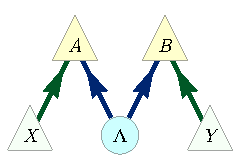
\includegraphics[scale=1]{BellDagRaw.pdf}
\caption{The causal structure of the a bipartite Bell scenario. The local outcomes of Alice's and Bob's experimental probing is assumed to be a function of some latent common cause, in addition to their independent local experimental settings.}\label{fig:NewBellDAG}
\end{minipage}
\hfill
\begin{minipage}[t]{0.45\linewidth}
\centering
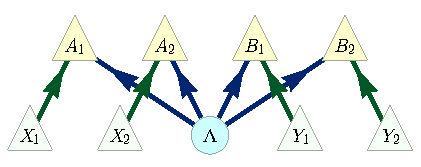
\includegraphics[scale=1]{BellDagCopy.pdf}
\caption{An inflation DAG of the bipartite Bell scenario, where both local settings variables have been duplicated.}\label{fig:BellDagCopy}
\end{minipage}
\end{figure}
\end{comment}

To further illustrate our inflation-DAG approach, we demonstrate how to recover all Bell inequalities \cite{Brunner2013Bell,bell1966lhvm,CHSHOriginal} via our method. To keep things simple we only discuss the case of a bipartite Bell scenario with two possible ``settings'' here, but the cases of more settings and/or more parties are totally analogous.
%It is critical that our method should be able to derive these seminal criteria, as Bell inequalities have been a foundational component of quantum information theory for the last half century \cite{scarani2012device,BancalDIApproach}.

Consider the causal structure associated to the Bell/CHSH \cite{bell1964einstein,Brunner2013Bell,bell1966lhvm,CHSHOriginal} experiment [\citealp{pusey2014gdag}~(Fig.~E\#2), \citealp{WoodSpekkens}~(Fig.~19), \citealp{chaves2014novel}~(Fig.~1), \citealp{BeyondBellII}~(Fig.~1), \citealp{wolfe2015nonconvexity}~(Fig.~2b), \citealp{steeg2011relaxation}~(Fig.~2)], depicted here in \cref{fig:NewBellDAG1}. The observable variables are $A,B,X,Y$, and $\Lambda$ is the latent common cause of $A$ and $B$.

In the Bell scenario DAG, one usually works with the conditional distribution $P(AB|XY)$, which is an array of distributions over $A$ and $B$ indexed by the possible values of $X$ and $Y$, instead of with the original distribution $P(ABXY)$. The maximal pre-injectable sets then are
\begin{align*}
\brackets{A_1 B_1, X_1 X_2 Y_1 Y_2} \\
\brackets{A_1 B_2, X_1 X_2 Y_2 Y_2} \\
\brackets{A_2 B_1, X_1 X_2 Y_2 Y_2} \\
\brackets{A_2 B_2, X_1 X_2 Y_2 Y_2} ,
\end{align*}
where we have put commas in order to clarify that every maximal pre-injectable set contains \emph{all} ``settings'' variables. Using These pre-injectables result in the given marginal distributions to take on the form
\begin{align*}
	P_{A_1 B_1 X_1 X_2 Y_1 Y_2}(a b x_1 x_2 y_1 y_2) & = P_{A B X Y}(a b x_1 y_1) P_X(x_2) P_Y(y_2), \\
	P_{A_1 B_2 X_1 X_2 Y_1 Y_2}(a b x_1 x_2 y_1 y_2) & = P_{A B X Y}(a b x_1 y_2) P_X(x_2) P_Y(y_1), \\
	P_{A_2 B_1 X_1 X_2 Y_1 Y_2}(a b x_1 x_2 y_1 y_2) & = P_{A B X Y}(a b x_2 y_1) P_X(x_1) P_Y(y_2), \\
	P_{A_2 B_2 X_1 X_2 Y_1 Y_2}(a b x_1 x_2 y_1 y_2) & = P_{A B X Y}(a b x_2 y_2) P_X(x_1) P_Y(y_1), \\
		P_{X_1 X_2 Y_1 Y_2}(x_1 x_2 y_1 y_2) & = P_X(x_1) P_X(x_2) P_Y(y_1) P_Y(y_2).
\end{align*}
Although the last equations follows from each of the others together with the Markov condition $P_{XY} = P_X P_Y$ for the original distribution, it nevertheless turns out to be useful to write down explicitly: putting $x_1 = y_1 = 0$ and $x_2 = y_2 = 1$ and dividing the first equation by the last one results in
\begin{align*}
	P_{A B X Y}(a b | 0 0)  =  \sum_{a',b'} P_{A_1 A_2 B_1 B_2 X_1 X_2 Y_1 Y_2}(aa'bb'|0101),
\end{align*}
and similarly also $P_{A B X Y}(a b | 0 1)$, $P_{A B X Y}(a b | 1 0)$ and $P_{A B X Y}(a b | 1 1)$ can be written as marginals of a conditional distribution. By Fine's Theorem~\cite{FineTheorem}, this implies the existence of a hidden-variable model. Conversely, if a hidden-variable model exists, then the existence of the inflation model implies the existence of a solution to the marginal problem. In conclusion, we therefore find in the case of the inflation DAG~\cref{fig:BellDagCopy1}, our method provides a necessary and sufficient condition for feasibility with the Bell causal structure. In particular, the marginal problem on this inflation DAG reproduces \emph{all} Bell inequalities.

\begin{comment}
Analysis of the inflated DAG in \cref{fig:BellDagCopy1} shows that 
\begin{align}\label{eq:bellypolymapped}
 \p{a b x y}\p{\n{x}} \p{\n{y}}
&\leq
 \p{a \n{b} x \n{y}}\p{\n{x}}\p{y} +  \p{\n{a} b \n{x} y}\p{x} \p{\n{y}}+\p{a b \n{x} \n{y}}\p{x} \p{y}
\\
\shortintertext{by virtue of the unmapped (but factored) inequality}
\label{eq:bellypolyunmapped}
 \p{a_1 b_1 x_1 y_1}\p{\n{x}_2} \p{\n{y}_2}
&\leq
 \p{a_1 \n{b}_2 x_1 \n{y}_2}\p{\n{x}_2} \p{y_1} +\p{\n{a}_2 b_1 \n{x}_2 y_1}\p{x_1}\p{\n{y}_2}+  \p{a_2 b_2 \n{x}_2 \n{y}_2}\p{x_1} \p{y_1}
\end{align}
where \emph{every} probability appearing in \cref{eq:bellypolyunmapped} maps to the original scenario, hence yielding \cref{eq:bellypolymapped}. To derive the usual Bell inequalities from \cref{eq:bellypolymapped} we switch to conditional probabilities via ${\p{a b x y}\to\p{a b | x y}\p{x y}=\p{a b | x y}\p{x}\p{y}}$ which, after dividing both sides of \cref{eq:bellypolymapped} by $\p{x}\p{\n{x}}\p{y}\p{\n{y}}$, yields
\begin{align}\label{eq:chwithneg}
&\p{a b | x y}
\leq
{\p{a \n{b} | x \n{y}} + \p{\n{a} b | \n{x} y}+\p{a b | \n{x} \n{y}}}
\\
\hspace{-\mathindent}\text{or, equivalently,}\quad
\label{eq:chwithoutneg}
&{\p{a b | x y}+\p{a b | x \n{y}} + \p{a b | \n{x} y}}
\leq
{\p{a|\n{x}}+\p{b|\n{y}} + \p{a b | \n{x} \n{y}}}
\end{align}
which is precisely the Clauser-Horne (CH) inequality \cite{CHInequality} for the Bell scenario. Note that to obtain \cref{eq:chwithoutneg} from \cref{eq:chwithneg} we implicitly made use of the no-signalling assumptions, namely $\p{a|x y}=\p{a|x}$ and $\p{b| x y}=\p{b | y}$. The CH inequality is the \emph{unique} Bell inequality (up to permutations) for the Bell scenario if $\brackets{A,B,X,Y}$ are all binary, and hence the CH inequality is a necessary and sufficient criterion to ascertain if correlations are compatible with that Bell scenario variant.

The causal structure of a Bell scenario can also be formulated directly in terms of conditional random variables. For example, the conditional-structure interpretation of \cref{fig:BellDagCopy1} is \cref{fig:BellConditionalDAG}. 

\begin{figure}[t]
\centering
\begin{minipage}[t]{0.45\linewidth}
\centering
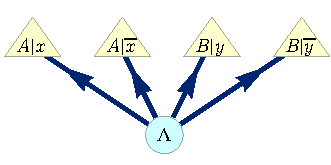
\includegraphics[scale=1]{BellDagConditionForm.pdf}
\caption{The causal structure of the Bell scenario expressed in a form which makes use of conditional random variables.}\label{fig:BellConditionalDAG}
\end{minipage}
%\hfill
%\begin{minipage}[t]{0.45\linewidth}
%\centering
%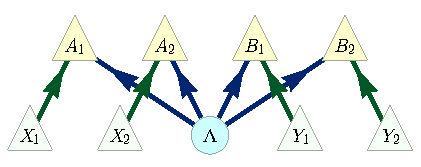
\includegraphics[scale=1]{BellDagCopy.pdf}
%\caption{An inflation DAG of the Bell scenario, where both local settings variables have been duplicated.}\label{fig:BellDagCopy}
%\end{minipage}
\end{figure}

The Bell inequalities are then self-evident from \cref{fig:BellConditionalDAG} without the need for an inflation DAG. The conditional-structure formulation innately implies its own inaccessible gedankenprobabilities, such as $\{\p{a|x , a|\n{x}}$, $\p{a|x , \n{a}|\n{x}},...\}$ etc. By eliminating these gedankenprobabilities from the set of inequalities generated by $0\leq \pdf{A|x , A|\n{x} , B|y , B|\n{y}}$ we obtain
\begin{align}\label{eq:bellcondeq}
0
\leq
{\p{a|\n{x}} + \p{b|\n{y}} + \p{a|x , b|y} -\p{a|x ,b|\n{y}} -\p{a|\n{x} , b|y} -\p{a|\n{x} , b|\n{y}}}\,,
\end{align}
for example. It should be clear that \cref{eq:bellcondeq} is equivalent to \cref{eq:chwithoutneg}.

%We can perform quantifier elimination on the set of (polynomial) inequalities given by $0\leq \pdf{A|x , A|\n{x} , B|y , B|\n{y}}$. The use of a conditional-structure DAG innately implies certain inaccessible gedankenprobabilities, such as $\{\p{a|x , a|\n{x}}$, $\p{a|x , \n{a}|\n{x}},...\}$ etc. 
\purp{Rob says kill next two paragraphs?}

Conditional-structure gedankenprobabilities are somewhat different from the inflation DAG kind, in that they reference multiple counterfactual events, such as ``What is the probability that Alice would choose to visit the museum \emph{IF} (given that) it's a rainy day in Maryland \emph{AND} that Alice would choose to go the beach \emph{IF} (given that) it's sunny in Maryland?". By contrast, unconditional gedankenprobabilities which live on an inflation DAG reference multiple heterofactual (for lack of a better word) events, such as ``What is the probability that Alice-copy-\#1 chooses to visit the museum \emph{AND} that it's raining in Maryland-copy-\#1 \emph{AND} that Alice-copy-\#2 chooses to go the beach \emph{AND} that it's sunny in Maryland-copy-\#2?". 

Joint counterfactual probabilities are experimentally inaccessible, just the same as joint heterofactual probabilities are. Suppose one could establish both Alice's propensity for going to the museum when it rains and her propensity for going to the beach when it's sunny. Even so, neither the joint counterfactual probability nor the joint heterofactual probability can be established from that limited data. For example, the value of the hidden variable ${\Lambda\cramp{=}\lambda}$ may influence Alice's willingness to get out of bed at all, or determine if she is on-call as a volunteer EMT on a particular day, or $\lambda$ might encode if Alice is travelling out-of-state. If we could measure $\p{a|x , \n{a}|\n{x}},...\}$ we might learn that Alice's likelihood of visiting the museum if it rains in Maryland is highly correlated with her likelihood of visiting the beach when it's sunny in Maryland. Or we might learn that those two counterfactual probabilities are relatively statistically independent. The ``hidden-ness" of the classical variable corresponding to the latent node shields the gedankenprobabilities from being determined. 
\end{comment}

\section{Gedankenprobabilities and the Quantum No-Broadcasting Theorem}\label{sec:classicallity}

It is worth emphasizing that broadcasting gedankenprobabilities %which are predicated on multiple counterfactual or heterofactual events 
are strictly classical constructs. If the latent node in the Bell scenario in \cref{fig:NewBellDAG1} is allowed to be a quantum resource $\mathcal{H}^{d_A\otimes d_B}$, for example, then broadcasting gedankendistributions such as $\pdf{A|x , A|\n{x},...}$ or $\pdf{A_1,A_2,...}$ are \tblue{physically prohibited} if the quantum state is suitably entangled.

More precisely, quantum states are governed by a no-broadcasting theorem \cite{NoCloningQuantum1996,NoCloningGeneral2006}: If half the state is sent to Alice and she performs some measurement on it, she fundamentally perturbs the state by measuring it. Post-measurement, that half of the state cannot be ``re-sent" to Alice, that she might re-measure it using a different measurement setting. As a consequence of the no-broadcasting theorem, in the inflation DAG picture a quantum state which was initially available to a single party cannot be distributed both to Alice-copy-\#1 and Alice-copy-\#2 in the way a classical hidden variable could be. More generally, there is an analogous no-broadcasting theorem in the regime of epistemically-restricted general probabilistic theories (GPTs) \cite{SpekkensToyTheory,NoCloningGeneral2006,Barnum2012GPT,Janotta2014GPT}, so that this impossibility also holds in many theories other than quantum theory.

This means that considerations on inflation DAGs cannot be used to derive quantum causal infeasibility criteria whenever a gedankenprobability presupposes the ability to broadcast a latent node's system. Broadcasting and non-broadcasting sets of variables are distinguished per \cref{eq:nonbroadcastinginflationDAG}.

%When analyzing GPT causal structures one may not assume that a joint probability distribution over observable variables is universally nonnegative if the set of observable variables has simultaneous meaning only under broadcasting of latent variables. This is in direct contrast to \cref{step:generateineqs} in \cref{sec:mainalgorithm}. 

Not every inflation requires broadcasting, however, and hence not every gedankenprobability is physically prohibited by quantum theory. 
%An inflation DAG is a \tblue{non-broadcasting inflation} whenever the children of every individual node in the inflation DAG $G'$ map injectively to the corresponding children of the mapped node in the original DAG $G$, i.e. $dmap\parenths*{\Ch[G']{X}}\subseteq\Ch[G]{dmap\parenths*{X}}$ for all $X\in\nodes{G'}$. 
\cref{fig:TriDagSubA2B1C1} is an example of a non-broadcasting inflation.
Constraints derived from non-broadcasting inflations are valid even in the GPT paradigm. Consequently the inequality in \cref{eq:tritrivial1}, which was derived from \cref{fig:TriDagSubA2B1C1}, is therefore a causal infeasibility criterion which holds for the Triangle scenario even when the latent nodes are allowed to be quantum states. This confirms our numerical computations, which indicated that~\eqref{eq:tritrivial1} does not have any quantum violations. The same is true for monogamy of correlations, per \cref{eq:monogomyofcorrelations}. Since the GHZ-type distribution~\cref{eq:ghzdistribution1} violates both of these inequalities, it is forbidden even per the relaxed GPT Triangle scenario, as was pointed out earlier. 

It might also be possible to derive quantum causal infeasibility criteria if one appropriately modifies \cref{step:generateineqs} to generate a different initial set of nonnegativity inequalities. This new set should capture the nonnegativity of only quantum-physically-meaningful marginal probability distributions. From this perspective, a broadcasting inflation DAG is an abstract logical concept, as opposed to a hypothetical physical construct. Indeed, the distributions in a quantum broadcasting inflation DAG can be characterized in terms of the logical broadcasting maps of \citet{Coecke2011}. Note that $\p{a_1,a_2}$ and other broadcasting-implicit gedankenprobabilities can be \emph{negative} pursuant to a logical broadcasting map, and hence \cref{step:generateineqs} in \cref{sec:mainalgorithm} would need to be modified.

An analysis along these lines has already been carried out successfully by \citet{Chaves2015infoquantum} in the derivation of entropic inequalities for non-classical causal structures. Although \citet{Chaves2015infoquantum} do not invoke inflation DAGs, they do employ conditional structure, which therefore gives rise to broadcasting sets. \citet{Chaves2015infoquantum} take pains to avoid including broadcasting gedankenentropies in any of their initial entropic inequalities, precisely as we would want to do in constructing our initial probability inequalities. Unlike entropic inequalities, the derivation of probability inequalities has not yet been achieved for non-classical causal structures other than Bell scenarios. 

Our current inflation DAG method can be employed to derive causal infeasibility criteria for general causal structures, thus generalizing Bell inequalities somewhat. From a quantum foundations perspective, however, generalizing Tsirelson inequalities \cite{Tsirelson1980,Brunner2013Bell}---the ultimate constraints on what quantum theory makes possible---is even more desirable. Deriving additional quantum causal infeasibility criteria for general causal structure is therefore a priority for future research. \purp{T: move this to conclusions?}


\section{Tautologies of the Supplemented Excluded Middle}\label{sec:TSEM}

The process of linear quantifier elimination, while orders of magnitude more computationally amenable than its nonlinear variant, is nevertheless nontrivial. When the number of observable random variables in the inflation DAG is too large, it quickly happens that even the linear quantifier elimination algorithms may be too slow for practical application. To this end we have developed a strategy that identifies only one particular class of causal infeasibility criteria, but does so nearly instantly.

In this approach we construct polynomial inequalities corresponding to some tautology of the excluded middle (TEM). In classical logic, the TEM refers to that self-evident truism that every proposition is either true or false, and hence 
\begin{align}
\mathsf{True} \iff \NamedFunction{Or}{ A\cramp{=}a , A\cramp{\neq}a }\,.
\end{align}
Note that we treat statistical events such as random variables yielding particular outcomes as identically logical propositions. The TEM can also be supplemented with certain ``givens", which we take to be known-true propositions on the left-hand-side. These ``givens" can then be interspersed throughout the right-rand-side while still yielding a valid tautology. Thus
\begin{align}\label{eq:TSEMdemo}
\NamedFunction{And}{ \mgreen{a} , \mgreen{b} }
\implies 
\NamedFunction{Or}{
    \NamedFunction{And}{ \mgreen{a} , c } ,\\
    \NamedFunction{And}{ \mgreen{b} , \n{c} }
}
\end{align}
is an example of a tautology of the \emph{supplemented} excluded middle (T\emph{S}EM). For pedagogical clarity we color and bold the ``given" outcomes on both sides of the tautology.

Every TSEM can be converted into a linear inequality by virtue of two connections between classical logical and probability:
\begin{compactenum}
\item As the antecedent always implies the consequent, the probability of the antecedent is necessarily less-than-or-equal-to the probability of the consequent. If $j \cramp{\scriptstyle \implies} k$ then $\p{j}\leq\p{k}$.
\item The probability of a disjunction of events is less-than-or-equal-to the sum of the probabilities of the individual events, i.e. ${\p{j\lor k}=\p{j}+\p{k}-\p{j,k}\leq \p{j}+\p{k}}$.
\end{compactenum}
The inequality which would correspond to the TSEM in \cref{eq:TSEMdemo} is 
\begin{align}
    \p{a b} \leq \p{a c}+\p{b \n{c}}\,.
\end{align}

TSEM inequalities can be used as precursors for polynomial inequalities by applying them to inflation DAGs. For example the TSEM inequality
\begin{align}
    \p{a_2 b_1} \leq \p{a_2 b_1}+\p{\n{b}_1 c_1}
\end{align}
applied to our inflation of the Triangle scenario would imply the causal infeasibility criterion  
\begin{align}
    \p{a}\p{c} \leq \p{a b}+\p{\n{b} c}
\end{align}
pursuant to \cref{fig:TriDagSubA2B1C1}.

In fact almost every causal infeasibility criterion in this paper is a TSEM inequality! The Triangle scenario inequality \cref{eq:trifancyunmapped} corresponds to the logical TSEM
\begin{align}
    \NamedFunction{And}{\mgreen{a_2} , \mgreen{b_2} , \mgreen{c_2}}\implies 
\NamedFunction{Or}{\NamedFunction{And}{\n{a}_1 , \n{b}_1 , \n{c}_1},\\ \NamedFunction{And}{a_1 , \mgreen{b_2} , \mgreen{c_2}},\\ \NamedFunction{And}{\mgreen{a_2} , b_1 , \mgreen{c_2}},\\ \NamedFunction{And}{\mgreen{a_2} , \mgreen{b_2} , c_1}}
\end{align}
and then Bell scenario inequality in \cref{eq:bellypolyunmapped} follows from the logical TSEM
\begin{align}
 \NamedFunction{And}{\mgreen{a_1} , \mgreen{b_1} , \mgreen{x_1} , \mgreen{\n{x}_2}, \mgreen{y_1} ,  \mgreen{\n{y}_2}}
\implies
\NamedFunction{Or}{\NamedFunction{And}{\n{a}_2 , \mgreen{b_1} , \mgreen{x_1}, \mgreen{\n{x}_2} , \mgreen{y_1} , \mgreen{\n{y}_2}}\\
\NamedFunction{And}{\mgreen{a_1} , \n{b}_2 , \mgreen{x_1} ,\mgreen{\n{x}_2},\mgreen{y_1},\mgreen{\n{y}_2}}\\
\NamedFunction{And}{a_2 , b_2 , \mgreen{x_1}, \mgreen{\n{x}_2}, \mgreen{y_1}, \mgreen{\n{y}_2}}}
\end{align}
etc.

Generating TSEM inequalities is computationally much easier than performing quantifier elimination. A practical alternative to \cref{sec:mainalgorithm}, then, is the four-step process
\begin{compactenum}
\item Generate TSEM inequalities on the inflation DAG.
\item Factor the probabilities (same as \cref{step:fac} in \cref{sec:mainalgorithm}).
\item Map as many probabilities to the original DAG as possible (same as \cref{step:findmap} in \cref{sec:mainalgorithm}).
\item Discard any remaining inequalities which involve unmappable gedankenprobabilities.
\end{compactenum}
Restricting one's search to TSEM inequalities makes deriving causal infeasibility criteria extremely tractable even for large DAGs, but a consequence, however, is that only one class of possible inequalities is being considered.

In order to make a TSEM inequality as compelling as possible one should ensure that every event on the left hand side is also referenced at least once on the right hand side. If one find a TSEM inequality lacking this property then one should tighten the inequalities by deleting any events which occur only on the left hand side. This preserves the tautology while increasing the probability of the left hand side.

We note that the connection between classical propositional logic and linear inequalities has been used previously in the task of causal inference. We reiterate that inequalities resulting from propositional logic, however, are a subset of the inequalities that result from linear quantifier elimination. Consequently, linear quantifier elimination is the preferable tool for deriving inequalities whenever the elimination is computationally tractable. Noteworthy examples of works deriving causal infeasibility criteria via classical logic are \citet{Pitowsky1989} and \citet{Ghirardi08}: \cref{eq:trisimplestunmapped} here corresponds to Eq. (2-4) in Ref. \cite{Pitowsky1989}, and \cref{eq:bellcondeq} here corresponds to Eq. (30) in Ref. \cite{Ghirardi08}.






\section{Conclusions}
%\purp{Not yet written. To discuss: 
%\begin{compactitem}
%\item Relations to other work.
%\item Why linear elimination is weaker than nonlinear. 
%\item Why a single inflation DAG yields necessary but not sufficient inequalities. 
%\item Why not maximal degree yet known on inequalities. 
%\item Extent to which quantum latent variables violate these inequalities as desideratum for future research.
%\end{compactitem}
%}

%\begin{spacing}{2.0}
Our main contribution is a new way of deriving causal infeasibility criteria, namely the inflation DAG approach. An inflation DAG naturally implies nonlinear hybrid inequalities, i.e. containing gedankenprobabilities, which implicitly constrain the set of distribution consistent with the original causal structure. If desirable, one can further eliminate the gedankenprobabilities via quantifier elimination. Polynomial inequalities can be obtained through linear elimination techniques.

These inequalities are necessary but not sufficient conditions on a joint distribution for it to be explained by the causal structure. We've seen that they can be stronger than entropic inequalities sometimes, yet just how strong they are is still unclear. A distribution might satisfy all our polynomial inequalities and yet not be realizable from the causal structure. %What would such superficially-feasible distributions look like? Are inflation DAG inequalities ever tight? 
Our methods yields tight causal infeasibility criteria for Bell scenarios, but those scenarios are exceptional in that the sets of realizable distributions form a convex polytope.

The most elementary of all causal infeasibility criteria are the conditional independence (CI) relations. Our method explicitly incorporates all marginal independence relations implied by a causal structure. We have found that generic CI relations also appear to be implied by our polynomial inequalities. In future research we hope to clarify the process through which CI relations are manifested as properties of the inflation DAG.

A single causal structure has unlimited potential inflations. Selecting the right inflation from which to derive polynomial inequalities is an interesting challenge. To this end, it would be desirable to understand how particular features of the original causal structure are exposed when different nodes in the DAG are duplicated. By isolating which features are exposed in each inflation we could conceivably quantify the causal inference strength of each inflation. In so doing, we might find that inflated DAGs beyond a certain level of variable duplication need not be considered. The multiplicity beyond which further inflation is irrelevant is presumably related to the maximum degree of those polynomials which tightly characterize a causal scenario. Presently, however, it is not clear how to upper bound either number.

%that one inflation DAG is or is not ``stronger" than another? Can we upper bound the maximum dimension of those polynomials which in-principle tightly characterize a given causal structure? A ``yes" answer to any of the aformentioned questions means that that perhaps inflation DAGs beyond a certain level of complexity need not be considered. These remain open questions, however.

Our method turns the quantum no-broadcasting theorem \cite{NoCloningQuantum1996,NoCloningGeneral2006} on its head by emphasizing that classical hidden variables \emph{can}, in-principle, be cloned. This classical cloning possibility motivates the inflation DAG method, and underpins the implied causal infeasibility criteria. We have speculated about generalizing our method to obtain causal infeasibility criteria that constitute necessary constraints even for \emph{quantum} causal scenarios, a common desideratum in recent works \cite{fritz2012bell,pusey2014gdag,Chaves2015infoquantum,ChavesNoSignalling,BeyondBellII}. It would be enlightening to understand the extent to which our (classical) polynomial inequalities are violated in quantum theory. A variety of techniques exist for estimating the amount by which a linear inequality \cite{NPA2008Long,I3322NPA1} is violated in quantum theory, but finding the quantum violation of a \emph{polynomial} inequality is a more challenging task \cite{NPAReview}.

The difference between classical ontic-state duplication and quantum no-broadcasting makes the inequalities that result from our consideration to be especially suited for distinguishing the set of quantum-realizable distributions from its subset of classically-realizable distributions. Causal infeasibility criteria that are sensitive to the classical-quantum distinction are precisely the sort of generalizations of the Bell inequalities which are sought after, in order to study the quantum features of generalized causal scenarios. Entropic inequalities have been lacking in this regard \cite{fritz2012bell,pusey2014gdag,Chaves2015infoquantum}, and the inflation DAG considerations proposed here constitute a significant alternative strategy.
%\end{spacing}





\begin{acknowledgments}
%\bigskip\noindent\textbf{Acknowledgments}
Research at Perimeter Institute is supported by the Government of Canada through Industry Canada and by the Province of Ontario through the Ministry of Economic Development and Innovation.
\end{acknowledgments}


\onecolumngrid
\appendix
\renewcommand{\theequation}{A-\arabic{equation}}
\setcounter{equation}{0}

\section{Nonlinear Quantifier Elimination Approach}\label{sec:nonlinearelimination}
In the main text we considered deriving constraints on the pre-injectable sets via the marginal problem. There are further implications in the inflation DAG, however, which can be leveraged to further constrain the marginal distributions consisted with the inflation DAG.

\begin{asparadesc}
\medskip\item[\tred{Conditional Independence Relations}] \noindent
\par\hspace{\parskip} 
The most familiar such further constraints are the conditional independence relations relating observable variables in the inflation DAG. Conditional independence relations are inferred by $d$-separation; if $\bm{X}$ and $\bm{Y}$ are $d$-separated in the (inflation) DAG by $\bm{Z}$, then we infer $\bm{X}\bot\bm{Y}|\bm{Z}$. The $d$-separation criterion is explained at length in Refs. \cite{pearl2009causality,studeny2005probabilistic,WoodSpekkens,pusey2014gdag}, we present it only informally here.

We first define the notion of \tblue{exclusive ancestors}, because the usual notion of ancestors is inclusive, i.e. $\An{\bm{Z}}$ contains $\bm{Z}$. Let the exclusive ancestors of $\bm{Z}$ so that $\An{\setminus\bm{Z}}\coloneqq\An{\bm{Z}}\setminus\bm{Z}$. Next we define \tblue{conditioning a DAG} over $\bm{Z}$, i.e. $G_{\setminus\bm{Z}}$, which is formed by deleting any outgoing edges from $\bm{Z}$ in $G$. Conditional DAGs enable the definition of \tblue{conditional ancestors}, i.e. 
\begin{align}
    \An[G]{\bm{X}|\bm{Z}}\coloneqq \begin{cases}
    \An[G_{\setminus\bm{Z}}]{\bm{X}}& \text{if } \An[G_{\setminus\bm{Z}}]{\bm{X}} and \An[G]{\setminus\bm{Z}} are disjoint\\
    \An[G_{\setminus\bm{Z}}]{\bm{X}} \bigcup \An[G]{\setminus\bm{Z}} & \text{if } \An[G_{\setminus\bm{Z}}]{\bm{X}} and \An[G]{\setminus\bm{Z}} overlap.
    \end{cases}
\end{align}
Finally, $\bm{X}$ and $\bm{Y}$ are $d$-separated by $\bm{Z}$ iff $\An[G]{\bm{X}|\bm{Z}}$ and $\An[G]{\bm{Y}|\bm{Z}}$ are disjoint.

Every conditional independence relation can be translated into a nonlinear constraint on probabilities, as $\bm{X}\bot\bm{Y}|\bm{Z}$ implies $\p{\bm{x}\bm{y}|\bm{z}}=\p{\bm{x}|\bm{z}}\p{\bm{y}|\bm{z}}$ for all $\bm{x}$, $\bm{y}$, and $\bm{z}$. As we generally prefer to work with unconditional probabilities, we summarize as follows: If $\bm{X}$ and $\bm{Y}$ are $d$-separated by $\bm{Z}$ then $\p{\bm{x}\bm{y}\bm{z}}\p{\bm{z}}=\p{\bm{x}\bm{z}}\p{\bm{y}\bm{z}}$ for all $\bm{x}$, $\bm{y}$, and $\bm{z}$. Such nonlinear constraints can be incorporated as restrictions on distributions consistent with the inflation DAG, supplementing the more trivial marginal-problem type constraints, and hence implicitly further constraining the injectable sets. Nonlinear quantifier elimination can then be used to make the implied constraints explicit.

Many modern computer algebra systems have functions capable of tackling nonlinear quantifier elimination symbolically\footnote{For example \textit{Mathematica$^{_{\textit{\tiny\texttrademark}}}$}'s \href[pdfnewwindow]{http://reference.wolfram.com/language/ref/Resolve.html}{\texttt{Resolve}} command, \textit{Redlog}'s \href[pdfnewwindow]{http://www.redlog.eu/documentation/reals/rlqe.php}{\texttt{rlposqe}}, or \textit{Maple$^{_{\textit{\tiny\texttrademark}}}$}'s \href[pdfnewwindow]{http://maplesoft.com/support/help/Maple/view.aspx?path=RegularChains/SemiAlgebraicSetTools/RepresentingQuantifierFreeFormula}{\texttt{RepresentingQuantifierFreeFormula}}, etc.}. 
%One might then hope to use such software systems to rid the hybrid inequalities of the gedankenprobabilities. 
Currently, however, it is not practical to perform nonlinear quantifier elimination on large polynomial systems with many quantifiers. Nevertheless, the nonlinear constraints can be easily accounted for numerically. Upon substituting numeric values for all the injectable probabilities the former quantifier elimination problem is converted to a universal quantifier existence problem: Do there exist gedankenprobabilities that satisfy the full set of linear and nonlinear constraints? Most computer algebra systems can resolve such \emph{satisfiability} questions quite rapidly\footnote{For example \textit{Mathematica$^{_{\textit{\tiny\texttrademark}}}$} \href[pdfnewwindow]{http://reference.wolfram.com/language/Experimental/ref/ExistsRealQ.html}{\texttt{Reduce\`{}ExistsRealQ}} function. Specialized satisfiability software such as SMT-LIB's \href[pdfnewwindow]{http://smtlib.cs.uiowa.edu/solvers.shtml}{\texttt{check-sat}} \cite{BarFT-SMTLIB} are particularly apt for this purpose. One can also exploit the fact than any nonlinear optimizer will return an error when a set of constraints cannot be satisfied. Nonlinear optimizers include \textit{Maple$^{_{\textit{\tiny\texttrademark}}}$}'s \href[pdfnewwindow]{http://www.maplesoft.com/support/help/Maple/view.aspx?path=Optimization/NLPSolveMatrixForm}{\texttt{NLPSolve}}, \textit{Mathematica$^{_{\textit{\tiny\texttrademark}}}$}'s \href[pdfnewwindow]{http://reference.wolfram.com/language/ref/message/NMinimize/nsol.html}{\texttt{NMinimize}}, and dozens of free and commercial optimizers for \href[pdfnewwindow]{http://ampl.com/products/solvers/all-solvers-for-ampl}{\textit{AMPL}} and/or \href[pdfnewwindow]{https://neos-server.org/neos/solvers/index.html\#nco}{\textit{GAMS}}}.

\begin{table*}[ht]\centering\caption{A comparison of different approaches constraining the pre-injectable sets. The primary divide is quantifier elimination versus quantifier existence, with approaches being further subdivided into linear and nonlinear variants.}
\begin{tabularx}{\linewidth}{ |l|L|c|L| } 
\hline
Approach & Also Known As & Difficulty & End Results \\
\bottomrule
Nonlinear Quantifier Elimination & Resolving Partial Existential Closure & Very Hard & Necessary-but-not-Sufficient Polynomial Inequalities \\
\hline
Nonlinear Quantifier Satisfiability & Universal Existential Closure,\newline Nonlinear Programming & Easy & Certify the infeasibility of a specific distribution \\
\hline
Linear Quantifier Elimination & Polytope Projection & Moderate & Necessary-but-not-Sufficient Polynomial Inequalities \\
\hline
Linear Quantifier Satisfiability & Linear Programming,\newline Universal Existential Closure & Very Easy & Certify the infeasibility of a specific distribution \\
\hline
Alternate: Logical Tautologies & Combinatorial / Set-Theoretic Implications\newline Partial Marginal Problem & Easy & Necessary-but-not-Sufficient Polynomial Inequalities 
\\\toprule
\end{tabularx}
\end{table*}

It is also possible to use a mixed strategy of linear and nonlinear quantifier elimination, such as \citet{ChavesPolynomial} advocates. The explicit results of Ref. \cite{ChavesPolynomial} are therefore consequences of any inflation DAG, achieved by applying a mixed quantifier elimination strategy.

\medskip\item[\tred{Coinciding Marginal Distributions}] \noindent







In principle one can exploit any $d$-separation criteria from the inflation DAG in order to transform or supplement the inequalities. If $\bm{X}$ and $\bm{Y}$ are $d$-separated by $Z$, then $\p{\bm{x} \bm{y} \bm{z}}=\frac{\p{\bm{x}\bm{z}}\p{\bm{y}\bm{z}}}{\p{\bm{z}}}$ \cite{pearl2009causality,spirtes2011causation,studeny2005probabilistic,koller2009probabilistic}.


\purp{At the moment this is just a text dump from the earlier manuscript. Needs extensive cleanup!!!}





These are the kinds of equalities and inequalities we can make use of. 
\purp{Move to last? These are sort of optional - we don't actually use them...} Just as ancestral independence of nodes implies marginal independence of variables, so too $d$-seperation of nodes implies conditional independence. If $\bm{X}$ and $\bm{Y}$ are don't share a common ancestor, then ${\forall_{x y}\;\p{\bm{x} \bm{y} }=\p{\bm{x}}\p{\bm{y}}}$. If $\bm{X}$ and $\bm{Y}$ are $d$-separated by $Z$, then ${\forall_{xy z}\;\p{\bm{x} \bm{y} \bm{z}}\p{\bm{z}}=\p{\bm{x}\bm{z}}\p{\bm{y}\bm{z}}}$ \cite{pearl2009causality,spirtes2011causation,studeny2005probabilistic,koller2009probabilistic}. For example, in \cref{fig:Tri222}
\begin{align}\begin{split}\label[eqs]{eqs:dfac222_v2}
\larray{
A_2\aindep\{B_1,C_2\}\\
B_2\aindep\{A_2,C_1\}\\
C_2\aindep\{A_1,B_2\}
}\qquad\text{implies that}\qquad
\larray{
\pdf{A_1 A_2 B_2 C_2}=\pdf{C_2}\times\pdf{A_1 A_2 B_2}\\
\pdf{A_2 B_1 B_2 C_2}=\pdf{A_2}\times\pdf{B_1 B_2 C_2}\\
\pdf{A_2 B_2 C_1 C_2}=\pdf{B_2}\times\pdf{A_2 C_1 C_2}\\
\pdf{A_2 B_2 C_2}=\pdf{A_2}\times\pdf{B_2}\times\pdf{C_2}\\
}
\end{split}\end{align}
To be clear, each equality in \cref{eqs:dfac222_v2} implies many more equalities at the level of individual probabilities, such as ${\p{a_2 b_1 b_2 c_2}= \p{a_2} \p{b_1 b_2 c_2}}$, ${\p{a_2 b_1 b_2}= \p{a_2} \p{b_1 b_2}}$, ${\p{a_2 b_1}= \p{a_2} \p{b_1}}$, etc. 



\end{asparadesc}


-------------------------
Deriving polynomial inequalities can be done in four steps. 
\begin{compactenum}
\item Construct linear non-negativity inequalities.
\item Convert the inequalities to nonlinear ones via conditional independence relations.
\item Use injectable sets to connect the inequalities to the original DAG.
\item Perform quantifier elimination.
\end{compactenum}

\step{: \tred{Generate an initial set of linear inequalities}}\label{step:generateineqs}\par\smallskip\nobreak

\purp{TODO: Change to EQUATIONS and inequalities, so that the inequality-only picture follows from the original one... UNDERWAY. EDITS IN PROGRESS HERE.} 

In order to derive inequalities on the original DAG, we begin by composing a set of linear conditions pertaining to the observable variables in the inflated DAG. Let the initial set be the nonnegativity of probability for all possible assignments to all observable variables. For simplicity, we take all observable variables to be binary, but the derivation can easily be adjusted to account for any number of outcomes. Taking the six observable variables in \cref{fig:Tri222} to be binary, however, lead to 64 distinct nonnegativity conditions, corresponding to $0\leq \pdf{A_1 A_2 B_1 B_2 C_1 C_2}$. The starting nonnegativity inequalities therefore look like
\begin{align}
\begin{split}
 0&\leq \p{a_1 a_2 b_1 b_2 c_1 c_2} \\
 0&\leq \left[\p{\n{a}_1 a_2 b_1 b_2 c_1 c_2}=\right]{\p{a_2 b_1 b_2 c_1 c_2} -\p{a_1 a_2 b_1 b_2 c_1 c_2}} \\
  0&\leq \left[\p{a_1 \n{a}_2 b_1 b_2 c_1 c_2}=\right]{\p{a_1 b_1 b_2 c_1 c_2} -\p{a_1 a_2 b_1 b_2 c_1 c_2}} \\
 \MTFlushSpaceAbove&{\vdots}\MTFlushSpaceBelow
 0&\leq \left[\p{\n{a}_1 \n{a}_2 b_1 b_2 c_1 c_2}=\right]{\p{b_1 b_2 c_1 c_2} -\p{a_1 b_1 b_2 c_1 c_2} -\p{a_2 b_1 b_2 c_1 c_2} + \p{a_1 a_2 b_1 b_2 c_1 c_2}}\\
  0&\leq \left[\p{\n{a}_1 a_2 \n{b}_1 b_2 c_1 c_2}=\right]{\p{a_2 b_2 c_1 c_2} -\p{a_1 a_2 b_2 c_1 c_2} -\p{a_2 b_1 b_2 c_1 c_2} + \p{a_1 a_2 b_1 b_2 c_1 c_2}}\\
 \MTFlushSpaceAbove
&{\vdots}
\MTFlushSpaceBelow
\end{split}
\end{align}
etc. These inequalities are found by iterating over the general definition of 
$\p{\bm{x} \n{\bm{y}}}=\p{\bm{x}}-\p{\bm{x} \bm{y}}$
applied to all possible joint probabilities.

%\begin{description}\itemsep0pt
%            \item[\textbf{Step 2}]\label[step]{step:fac} Find Factorization Relations from the Inflated DAG
%\end{description}
\step{: \tred{Infer factorization of probabilities from structural independence}}\label{step:fac}\par\smallskip\nobreak
These ``trivial" linear inequalities on the inflated DAG can be made into (weak) nontrivial polynomial inequalities by accounting for the marginal independence of certain random variable subsets. Independence of various distributions implies factorization of joint probabilities; the factorization of probabilities is the first step in transforming our set of otherwise-linear conditions.

We inspect the inflated DAG to find pairwise ancestral independences. In \cref{fig:Tri222}, for example, there are six pairs of ancestrally independent individual nodes, which consequently imply many marginal independences.
\begin{align}\begin{split}\label[eqs]{eq:dfac222}
\larray{
A_2\aindep\{B_1,C_2\}\\
B_2\aindep\{A_2,C_1\}\\
C_2\aindep\{A_1,B_2\}
}\qquad\text{implies that}\qquad
\larray{
\pdf{A_1 A_2 B_2 C_2}=\pdf{C_2}\times\pdf{A_1 A_2 B_2}\\
\pdf{A_2 B_1 B_2 C_2}=\pdf{A_2}\times\pdf{B_1 B_2 C_2}\\
\pdf{A_2 B_2 C_1 C_2}=\pdf{B_2}\times\pdf{A_2 C_1 C_2}\\
\pdf{A_2 B_2 C_2}=\pdf{A_2}\times\pdf{B_2}\times\pdf{C_2}\\
}
\end{split}\end{align}
etc.
Interestingly, the original DAG in \cref{fig:TriMainDAG} does not imply any observable marginal independence relations, nor any observable conditional independence relations at all, for that matter. 

By accounting for marginal independence relations, the set of linear inequalities is transformed into a set of polynomial inequalities. \cref{eq:dfac222} imply factorization of many different probabilities, such as ${\p{a_2 b_1 b_2 c_2}= \p{a_2} \p{b_1 b_2 c_2}}$, ${\p{a_2 b_1 b_2}= \p{a_2} \p{b_1 b_2}}$, ${\p{a_2 b_1}= \p{a_2} \p{b_1}}$, etc. In principle one can exploit any $d$-separation criteria from the inflation DAG in order to transform or supplement the inequalities. If $\bm{X}$ and $\bm{Y}$ are $d$-separated by $Z$, then $\p{\bm{x} \bm{y} \bm{z}}=\frac{\p{\bm{x}\bm{z}}\p{\bm{y}\bm{z}}}{\p{\bm{z}}}$ \cite{pearl2009causality,spirtes2011causation,studeny2005probabilistic,koller2009probabilistic}. For simplicity, however, we have restricted our attention here to exclusively ancestral independences. 



%\begin{description}\itemsep0pt
%            \item[\textbf{Step 3}] Find Map from Inflated DAG to Original DAG
%\end{description}
\step{: \tred{Map marginal distributions in the inflated DAG to those in the original structure}}\label{step:findmap}\par\smallskip\nobreak

Here we account for injectable sets. As any subset of an injectable set is also an injectable set, we enumerate here only \emph{maximal} injectable sets. The maximal injectable sets in \cref{fig:Tri222} are
\begin{align}
\begin{array}{l}
\brackets{A_1 B_2},\\
\brackets{B_1 C_2},\\
\brackets{A_2 C_1},\\
\text{and }\brackets{A_1 B_1 C_1},
\end{array}
\quad\text{which in turn imply that}\quad
\begin{array}{l}\label[eqs]{eq:dmap222}
%&\NamedFunction{PDF}{\!A_1,B_2\!}=\NamedFunction{PDF}{\!A,B\!},\quad\NamedFunction{PDF}{\!B_1,C_2\!}=\NamedFunction{PDF}{\!B,C\!},\quad\NamedFunction{PDF}{\!A_2,C_1\!}=\NamedFunction{PDF}{\!A,C\!},\\
%&\quad\NamedFunction{PDF}{\!A_1,B_1,C_1\!}=\NamedFunction{PDF}{\!A,B,C\!},
\pdf{A_1 B_2}=\pdf{A B},\\
\pdf{B_1 C_2}=\pdf{B C},\\
\pdf{A_2 C_1}=\pdf{A C},\\
\text{and }\pdf{A_1 B_1 C_1}=\pdf{A B C}.
\end{array}\end{align}

\begin{comment}
Recall that the random variables in the inflated DAG are constructed to be copies of the original random variables. As such, it is possible that two distinct subgraphs of the inflated DAG may represent precisely the \emph{same} causal structure, if the two subgraphs are equivalent up to ``dummy index" of the copied variables. Moreover, some subgraphs of the inflated DAG are equivalent to subgraphs of the original DAG, in the same sense of equivalent. When two graphs are equivalent in this sense we call them \tblue{copy equivalent}. Note that this notion of copy equivalence is stronger than merely graph isomorphism: For two causal structures to be copy equivalent there must exist an isomorphism between the graphs such that every random variables is mapped to itself or a copy of itself. \purp{With expanded notation moved up front, this discussion should be trimmed.}

Consider, now, two different subsets of observable random variables in the inflated DAG. Both subsets should be described by the same marginal probability distribution if the \tblue{ancestral subgraphs} of both sets are copy equivalent. We define the ancestral subgraph of a set of variables $\bm{V}$ to mean the subgraph of the causal structure containing $\bm{V}$'s complete causal history, i.e. $\NamedFunction{Ancestors}{\!\bm{V}\!}$. $\NamedFunction{Ancestors}{\!\bm{V}\!}$ refers to the set $\bm{V}$ along with any vertices that have a directed path to leading from them to $\bm{V}$. Thus the ancestral subgraph of $\bm{V}$ consists of the vertices $\NamedFunction{Ancestors}{\!\bm{V}\!}$ and all edges between them per the original graph. As an example: \cref{fig:Tri222} is the ancestral subgraph of \cref{fig:TriFullDouble} on the six observable variables $\{A_1 A_2 B_1 B_2 C_1 C_2\}$. The ancestral subgraph corresponding to observables $\brackets{A_1 B_2 C_1}$ is illustrated in \cref{fig:TriDagSubA1B2C1}. In contrast, the ancestral subgraph of $\brackets{A_1 B_1 C_1}$ is copy equivalent to \cref{fig:TriMainDAG}. When a set of variables admits partitioning into causally independent partitions, then the ancestral subgraph of that set will have unconnected components. An example of a multiple-components ancestral subgraph is \cref{fig:TriDagSubA2B1C2}, where ${A_2\,\bot\,\brackets{B_1 C_2}}$, as per \cref{eq:dfac222}.

\begin{figure}[t]
\centering
\begin{minipage}[b]{0.375\linewidth}
\centering
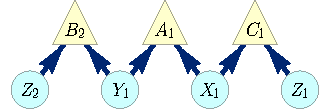
\includegraphics[scale=1]{TriDagSubA1B2C1.pdf}
\caption{A single-component ancestral subgraph of both \cref{fig:TriFullDouble,fig:Tri222}, consisting of observables $\brackets{A_1 B_2 C_1}$ and their complete causal histories. }\label{fig:TriDagSubA1B2C1}
\end{minipage}\hspace{80pt}
\begin{minipage}[b]{0.4\linewidth}
\centering
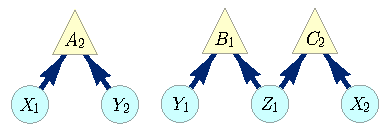
\includegraphics[scale=1]{TriDagSubA2B1C2.pdf}
\caption{A multiple-components ancestral subgraph of both \cref{fig:TriFullDouble,fig:Tri222}, consisting of observables $\brackets{A_2 B_1 C_2}$ and their complete causal histories. }\label{fig:TriDagSubA2B1C2}
\end{minipage}\hfill
\end{figure}

In sum: If two sets of random variables, $\bm{S}$ and $\bm{T}$, are equivalent up to their dummy indices AND the ancestral subgraphs of $\bm{S}$ and $\bm{T}$ are copy equivalent, then $\pdf{\bm{S}}=\pdf{\bm{T}}$. By inspecting different ancestral subgraphs for copy equivalence we can establish perfect equivalence of various marginal distributions. Coinciding marginal distributions reduces the number of parameters needed to describe the joint distribution over the entire inflated DAG. Multiple superficially distinct probabilities in the inflated DAG may actually share a single parameter. As an example, note that the marginal distributions over $\{A_1 A_2 B_1\}$ and $\{A_1 A_2 B_2\}$ must coincide, due to their copy-equivalent ancestral subgraphs. Consequently $\p{a_1 a_2 b_1}=\p{a_1 a_2 b_2}$, $\p{\n{a}_1 a_2 b_1}=\p{\n{a}_1 a_2 b_2}$, etc. The number of equivalent \emph{probabilities} implied by one pair of coinciding \emph{distributions} pertains to the (multivariate) range of the distributions. All the coincidences of marginal distributions implied by \cref{fig:Tri222} are given by
%$\NamedFunction{PDF}{\!A_1,A_2,B_1\!}=\NamedFunction{PDF}{\!A_1,A_2,B_2\!}$, $\NamedFunction{PDF}{\!A_1,C_1,C_2\!}=\NamedFunction{PDF}{\!A_2,C_1,C_2\!}$, and $\NamedFunction{PDF}{\!B_1,B_2,C_1\!}=\NamedFunction{PDF}{\!B_1,B_2,C_2\!}$.
\begin{align}\begin{split}\label[eqs]{eq:dequiv222}
%&\NamedFunction{PDF}{\!A_1,A_2,B_1\!}=\NamedFunction{PDF}{\!A_1,A_2,B_2\!},\quad\NamedFunction{PDF}{\!A_1,C_1,C_2\!}=\NamedFunction{PDF}{\!A_2,C_1,C_2\!},\\
%&\quad\NamedFunction{PDF}{\!B_1,B_2,C_1\!}=\NamedFunction{PDF}{\!B_1,B_2,C_2\!},
\pdf{A_1 A_2 B_1}=\pdf{A_1 A_2 B_2},\;\pdf{B_1 B_2 C_1}=\pdf{B_1 B_2 C_2},\;\pdf{A_1 C_1 C_2}=\pdf{A_2 C_1 C_2},
\end{split}\end{align}
%Nine pairs of Coinciding joint distributions in the inflated DAG \cref{fig:Tri222} lead to 
and their subsets.

To determine all marginal distribution coincidences we constructed the ancestral subgraph of every subset of observable random variables in the inflated DAG, and then picked out all copy equivalent pairings\footnote{Actually, the authors used a somewhat more efficient method to infer all marginal distribution coincidences. Discussing optimization is unwarranted, though, because this task is so easily accomplished by a computer.}. We note that \cref{step:fac} of finding marginally independent subsets can also be recast in terms of ancestral subgraphs: Sets of random variables $\bm{S}$ and $\bm{T}$ must be marginally independent if the ancestral subgraph of $\bm{S}$ does not intersect the ancestral subgraph of $\bm{T}$. This is illustrated in \cref{fig:TriDagSubA2B1C2}, where the ancestral subgraph of $A_2$ and the ancestral subgraph of $\{B_1 C_2\}$ comprise disconnected components in the ancestral subgraph of $\{A_2 B_1 C_2\}$.

In addition to such internal equivalency relations, we can further identify some marginal multivariate distributions in the inflated DAG which correspond to marginal distributions in the original DAG. The set of \emph{inter-DAG} marginal distribution coincidences may provide partial information regarding the set of \emph{intra-DAG}  marginal distribution coincidences; i.e. the set of inter-DAG probabilities-mapping relations effectually captures a subset of the intra-DAG probabilities-equivalency relations.  
The inter-DAG marginal distribution coincidences between \cref{fig:Tri222,fig:TriMainDAG} are
\begin{align}\begin{split}\label[eqs]{eq:dmap222}
%&\NamedFunction{PDF}{\!A_1,B_2\!}=\NamedFunction{PDF}{\!A,B\!},\quad\NamedFunction{PDF}{\!B_1,C_2\!}=\NamedFunction{PDF}{\!B,C\!},\quad\NamedFunction{PDF}{\!A_2,C_1\!}=\NamedFunction{PDF}{\!A,C\!},\\
%&\quad\NamedFunction{PDF}{\!A_1,B_1,C_1\!}=\NamedFunction{PDF}{\!A,B,C\!},
\pdf{A_1 B_2}=\pdf{A B},\;\pdf{B_1 C_2}=\pdf{B C},\;\pdf{A_2 C_1}=\pdf{A C},\;\pdf{A_1 B_1 C_1}=\pdf{A B C},
\end{split}\end{align}
and their subsets.
\end{comment}


The injectable sets allow us to transform our set of inequalities once more, this time into inequalities which have bearing on the original causal structure. We call this transformation of probabilities the \tblue{injection map}; the injection map pursuant to \cref{eq:dmap222} takes
\begin{align}\label[eqs]{eq:map222}
\underbrace{\begin{array}{l} \\
 \{\p{a_1}=\p{a_2}\}\to \p{a} \\
 \{\p{b_1}=\p{b_2}\}\to \p{b} \\
 \{\p{c_1}=\p{c_2}\}\to \p{c} 
\end{array}}_{\text{By the \emph{definition} of inflation.}}
\qquad\qquad
\underbrace{\begin{array}{l}
 \{\p{a_1 b_1}=\p{a_1 b_2}\}\to \p{a b} \\
 \{\p{a_1 c_1}=\p{a_2 c_1}\}\to \p{a c} \\
 \{\p{b_1 c_1}=\p{b_1 c_2}\}\to \p{b c} \\
 \p{a_1 b_1 c_1}\to \p{a b c} \\
\end{array}}_{\text{Via the injectable sets.}}
%\qquad
%\underbrace{\begin{array}{l} \\ 
% \{\p{a_1 a_2 b_1}=\p{a_1 a_2 b_2}\}\to \text{n/a} \\
% \{\p{a_1 c_1 c_2}=\p{a_2 c_1 c_2}\}\to \text{n/a} \\
% \{\p{b_1 b_2 c_1}=\p{b_1 b_2 c_2}\}\to \text{n/a} \\
%\end{array}}_{\text{Other intra-DAG equivalency relations}}
\end{align}
%Note that some - but far from all - of the \emph{internal} equivalency relations are captured by the inter-DAG equivalency conditions of \cref{eq:map222}. 

After applying the injection map  we are left we a system of \tblue{hybrid inequalities} of sorts, simultaneously containing two radically different kinds of probabilities. Some probabilities now pertain to the original DAG, but they appears alongside many probabilities which \emph{do not inject} to the original DAG. Probabilities which cannot be related to the original causal structure include $\{\p{a_1 b_1 c_2},\p{a_1 b_2 c_1},\p{a_2 b_1 c_1}\}$, and any joint probability which references more than one instance of a duplicated variable, such as $\{\p{a_1 a_2},\p{a_1 a_2 b_1},...\}$. The probabilities pertaining to the inflated DAG which have no parallel in the original DAG are precisely probabilities regarding non-injectable sets of variables.

We name these non-injectable probabilities \tblue{gedankenprobabilities}, as they could be measured in-principle if one were to physically construct the inflated causal structure\footnote{The inflated causal structure is always hypothetically constructable, classically, hence the though-experiment terminology. A gedankenprobability is also a well-defined hypothetical in quantum theory whenever the variables comprise a non-broadcasting set.}. As we are really only concerned with the original DAG, however, these ``unmeasured" joint distributions are effectively just thought experiments. The in-principle existence of gedankenprobabilities, however, is critical to inferring causal infeasibility criteria for the original DAG. 

As any superset of a non-injectable set is also not injectable, we enumerate here only \emph{minimal} non-injectable sets. The \emph{minimal} non-injectable sets in \cref{fig:Tri222} are
\begin{align}\label{eq:coreillegal222}
    \brackets{A_1 A_2},\quad\brackets{B_1 B_2},\quad\brackets{C_1 C_2},\quad\brackets{A_1 B_1 C_2},\quad\brackets{A_1 B_2 C_1},\quad\brackets{A_2 B_1 C_1}.
\end{align}
\cref{eq:coreillegal222} implies that our set of hybrid inequalities will be riddled with 34 different gedankenprobabilities.


%\begin{description}\itemsep0pt
%            \item[\textbf{Step 4}] Quantifier Elimination
%\end{description}
\step{: \tred{Quantifier elimination of the gedankenprobabilities}}\label{step:elimination}\par\smallskip\nobreak
We can infer implications for the original random variable from the system of hybrid inequalities obtained after \cref{step:findmap}. This inference task is essentially a form of quantifier elimination, where the quantifiers to be eliminated are the gedankenprobabilities. 
%Just the \emph{existence} of gedankenprobabilities such as $\p{a_1 a_2}$ can be used to imply constraints on the relevant probabilities \(\p{a}\), \(\p{b}\), \(\p{c}\), \(\p{a b}\), \(\p{a c}\), \(\p{b c}\), \(\p{a b c}\). 
Thus, the final step toward obtaining the desired causal infeasibility criteria is to eliminate the gedankenprobabilities from our system of hybrid polynomial inequalities. This quantifier elimination problem is well defined mathematically, although it is a challenging problem when the quantifiers are related nonlinearly. 

Many modern computer algebra systems have functions capable of tackling this sort of problem fully symbolically\footnote{For example \textit{Mathematica$^{_{\textit{\tiny\texttrademark}}}$}'s \href[pdfnewwindow]{http://reference.wolfram.com/language/ref/Resolve.html}{\texttt{Resolve}} command, \textit{Redlog}'s \href[pdfnewwindow]{http://www.redlog.eu/documentation/reals/rlqe.php}{\texttt{rlposqe}}, or \textit{Maple$^{_{\textit{\tiny\texttrademark}}}$}'s \href[pdfnewwindow]{http://maplesoft.com/support/help/Maple/view.aspx?path=RegularChains/SemiAlgebraicSetTools/RepresentingQuantifierFreeFormula}{\texttt{RepresentingQuantifierFreeFormula}}, etc.}. 
%One might then hope to use such software systems to rid the hybrid inequalities of the gedankenprobabilities. 
Currently, however, it is not practical to perform nonlinear quantifier elimination on large polynomial systems with many quantifiers. We consider, therefore, two other strategies for making effective use of the hybrid inequalities.

Firstly, one may substitute numeric values for all the injectable probabilities appearing in the polynomial inequality set. Upon doing so, the quantifier elimination problem is converted to a quantifier existence problem: Do there exist gedankenprobabilities that satisfy the resulting system of polynomial inequalities? Most computer algebra systems can resolve such \emph{satisfiability} questions quite rapidly\footnote{For example \textit{Mathematica$^{_{\textit{\tiny\texttrademark}}}$} \href[pdfnewwindow]{http://reference.wolfram.com/language/Experimental/ref/ExistsRealQ.html}{\texttt{Reduce\`{}ExistsRealQ}} function. Specialized satisfiability software such as SMT-LIB's \href[pdfnewwindow]{http://smtlib.cs.uiowa.edu/solvers.shtml}{\texttt{check-sat}} \cite{BarFT-SMTLIB} are particularly apt for this purpose. One can also exploit the fact than any nonlinear optimizer will return an error when a set of constraints cannot be satisfied. Nonlinear optimizers include \textit{Maple$^{_{\textit{\tiny\texttrademark}}}$}'s \href[pdfnewwindow]{http://www.maplesoft.com/support/help/Maple/view.aspx?path=Optimization/NLPSolveMatrixForm}{\texttt{NLPSolve}}, \textit{Mathematica$^{_{\textit{\tiny\texttrademark}}}$}'s \href[pdfnewwindow]{http://reference.wolfram.com/language/ref/message/NMinimize/nsol.html}{\texttt{NMinimize}}, and dozens of free and commercial optimizers for \href[pdfnewwindow]{http://ampl.com/products/solvers/all-solvers-for-ampl}{\textit{AMPL}} and/or \href[pdfnewwindow]{https://neos-server.org/neos/solvers/index.html\#nco}{\textit{GAMS}}}.

Note that real-world data with uncertainties can also be incorporated into these satisfiability questions. Instead of asserting that a particular probability is equal to a given \emph{value}, one can incorporate new inequalities which constrain the experimentally-known probabilities to lie in given \emph{intervals}. Assigning probabilities to intervals as opposed to numeric values results in further free parameters in the system, but the problem nevertheless remains one of \emph{universal} existential closure, and can be efficiently tested.




\section{Further Polytope Projection Algorithms}\label{sec:projalgorithms}

The Equality Set Projection (ESP) algorithm \cite{jones2004equality,JonesThesis2005} is ideal for handling inflation DAGs, because its computational complexity scales only according to the facet count of the final projection. Our use of larger-and-larger inflation DAGs to obtain causal infeasibility criteria on the same underlying original DAG means that while the complexity of the starting polytope is unbounded, the complexity of the projection is finite. Practically, this suggests that the ESP algorithm could parse the implications due to a very large inflation DAGs efficiently. Formally, ESP should require minimal computational overhead to consider a larger inflation DAG relative to considering a much smaller inflation DAG, when the \emph{implications} of the small and large inflations are similar. By contrast, the computation complexity of Fourier-Motzkin (FM) elimination algorithm scales with the number of quantifiers being eliminated. The number of gedankenprobabilities requiring elimination is exponentially related to the number of variables in the inflation DAG. The FM algorithm, therefore, is utterly impractical very for large inflation DAGs.

Another positive feature of the ESP algorithm is that it commences outputting quantifier-free inequalities immediately, and terminates upon deriving the complete set of inequalities. By contrast, FM works by eliminating one quantifier at a time. Terminating the ESP algorithm before it reaches completion would result in an incomplete list of inequalities. Even an incomplete list is valuable, though, since the causal infeasibility criteria we are deriving are anyways necessary but not sufficient.

Vertex projection (VP) algorithms are another computational tool which may be used to assist in linear quantifier elimination \cite{Avis2000lrs}. VP works by first enumerating the vertices of the initial polytope (H-rep to V-rep), projecting the vertices, and then converting back to inequalities (V-rep to H-rep). For generic high-dimensional polytopes, the operation of converting from a representation in terms of halfspaces to one in terms of extremal-vertices representations can be computationally costly (high-$d$ H-rep to V-rep). Starting from a vertex representation in a high dimensional space, however, one can immediately determine the vertex representation of the polytope's projection in a lower dimensional space. The projection is along the coordinate axes, so one just ``discards" the coordinate of the eliminated quantifier. To obtain the inequalities which characterize the projected polytope one then applies a convex hull algorithm to the projected vertices (low-$d$ V-rep to H-rep).

For probability distributions, however, the extremal vertices are precisely the deterministic possibilities. Since the extremal vertices of the initial polytope are easily enumerated, it is possible to avoid the high-$d$ V-rep to H-rep step entirely. There is a one-to-one correspondence between the inflation-DAG's initial generating inequalities and its initial extreme observable probability distributions. 
We used this V-rep to H-rep technique to project the initial polytope implied by \cref{fig:Tri222} (\cref{step:generateineqs}) to an intermediate 23-dimensional polytope, where each of the 23 remaining can be mapped the original DAG.  Only then did we apply the transformations of factorization and mappings (\cref{step:fac,step:findmap}) to convert those linear inequalities to polynomial inequalities pertaining to the original DAG. We found that the V-rep to H-rep technique, using \textit{lrs} [\href[pdfnewwindow]{http://cgm.cs.mcgill.ca/~avis/C/lrslib/USERGUIDE.html#Installation\%20Section}{\texttt{lrs}}], was orders-of-magnitude faster than FM elimination at obtaining the same result.

Yet another technique is also possible. Suppose the initial polytope is given by $\brackets{\vec{x},\vec{y}\,|\hat{A}.\vec{x}+\hat{B}.\vec{y}\geq\bm{c}}$, where $y$ are the quantifiers. If we can find any completely nonnegative vector $\bm{w}$ such that $\bm{w}.\hat{B}=\vec{0}$ then we automatically establish the quantifier-free inequality $\bm{w}.\hat{A}.\vec{x}\geq\bm{w}.\bm{c}$. Solving for ``random" nonnegative vectors $\bm{w}$ is easy; solving for all possible solutions is rather more difficult. \citet{BalasProjectionCone} refined this method so that each extremal construction of $\bm{w}$ corresponds to an irredundant inequality in the H-rep description of the projected polytope. Nevertheless, even without utilizing the full projection cone, this technique can be used to rapidly obtain a few quantifier-free inequalities. 

\section{Optimized Algorithm for Recognizing Redundant Inequalities}\label{sec:redundancy}
When performing Fourier-Motzkin linear quantifier elimination one must periodically filter out redundant inequalities from the set of linear inequalities. Equivalently, the means identifying redundant halfspace constraints in the description of the polytope. An individual constraint in a set is redundant if it is implied by the other constraints. 

An individual linear inequality is redundant if and only if it is a \emph{positive} linear combination of the others [Thm. 5.8 in \citealp{fordan1999projection}]\footnote{The ``if" is obvious. The ``only if" is a consequence of Farka's lemma \cite{fordan1999projection}.}. This is related to the V-rep characterization of polyhedral cones: If a cone is defined such that $W_{\hat{M}}\coloneqq\brackets{\vec{x}\,|\exists_{\bm{v}\geq\bm{0}}:\, \hat{M}.\bm{v}=\vec{x}}$ then $\vec{b}\in W_{\hat{M}}$ if and only if the linear system of equations $\hat{M}.\bm{v}=\vec{b}$ has a solution such that all the elements of $\bm{v}$ are nonnegative.  Thus, the computational tool required is one which accepts as input the matrix $\hat{M}$ and the column vector $\vec{b}$ and returns $\vec{b}\in W_{\hat{M}}$ as True or False. 


%It turns out that we can optimize the detection of redundant halfspaces when considering polyhedral cones as opposed to polytopes. Happily, the inequalities that pertain to the nonnegativity of probability describe a polytope which is identically the intersection of a cone with a hyperplane. The cone is given by the usual nonnegativity inequalities, just without defining $\p{}=1$. The hyperplane, then, is exactly $\p{}=1$. As the hyperplane-intersection constraint has no bearing on the quantifiers, we can set it aside, perform the projection, and then re-incorporate the $\p{}=1$ normalization condition after the Fourier-Motzkin procedure has completed.

%Consider a polyhedral cone with halfspace representation $W=\brackets{\vec{x}\,|\hat{A}.\vec{x}\geq \bm{0}}$. Each row in $\hat{A}$ is an inequality. Now consider the polar dual of $W$, namely $W^*=\brackets{\vec{x}\,|\exists_{\bm{v}\geq\bm{0}}:\, \hat{A}^{T}.\bm{v}=\vec{x}}$, in extremal-rays representation. Every halfspace (row of $\hat{A}$) in $W$ is associated with a ray (column of $\hat{A}^{T}$) in $W^*$. Critically, though, every irredundant halfspace in $W$ corresponds to an \emph{extremal} ray in $W^*$. Determining if a given ray is extremal or not is a computationally fast task. A ray in $W^*$ is \emph{not} extremal if it \emph{can} be expressed as a \emph{positive} linear combination of the other rays in $W^*$. \purp{Comment about one-to-one if $W$ is convex. Otherwise this trick detects only some, but not all, of the redundant inequalities. Also, citations needed.}

%Thus, the computational tool required is one which accepts as input the matrix $\hat{M}$ and the column vector $\vec{b}$, and which determines if the linear system of equations $\hat{M}.\bm{v}=\vec{b}$ has any solutions such that all the elements of $\bm{v}$ are nonnegative.

%For our purposes, $\hat{M}$ is the set of all rays \emph{other} than $\vec{b}$, where the columns of $\hat{M}$ are the other rays. 

Below, we present two possible \textit{Mathematica$^{_{\textit{\tiny\texttrademark}}}$} implementations which assess if a given column $\vec{b}$ can be expressed as a positive linear combination of the columns of $\hat{M}$. The former function is easy to understand, but the latter utilizes efficient low-level code and \textit{Mathematica$^{_{\textit{\tiny\texttrademark}}}$}'s internal error-handling to rapidly recognize infeasible linear programs.
\begin{align*}
 &\hspace{-\mathindent}\texttt{PositiveLinearSolveTest}[{M}\_?\texttt{MatrixQ},{b}\_]{:=}
 \texttt{With}[\{{vars}=\texttt{Thread}[\texttt{Subscript}[x,{\texttt{Dimensions}[{M}][[2]]}]]\},
 \\&\texttt{Resolve}[
 \texttt{Exists}[\texttt{Evaluate}[{vars}],\;
 \texttt{AllTrue}[{vars},\;\texttt{NonNegative}],
 \\&\texttt{And}\texttt{@@}\texttt{Thread}[{M}.\texttt{vars}==\texttt{Flatten}[{b}]]]]];
%\\\shortintertext{or, using efficient lower-level functions,}
       \\&\hspace{-\mathindent}\text{or}\quad\texttt{PositiveLinearSolveTest}[{M}\_?\texttt{MatrixQ},{b}\_]\texttt{/;Dimensions}[{b}]\texttt{===}\{\texttt{Length}[{M}],1\}{:=}
       \\&\hspace{-6ex}\texttt{Module}[\{{rowcount},{columncount},{fakeobjective},{zeroescolumn}\},
       \\&\hspace{-5ex}\{{rowcount},{columncount}\}=\texttt{Dimensions}[{M}];
       \\&\hspace{-5ex}{fakeobjective}=\texttt{SparseArray}[\{\},\{{columncount}\},0.0];
       \,{zeroescolumn}=\texttt{SparseArray}[\{\},\{{rowcount},1\}];
       \\&\hspace{-5ex}\texttt{Internal$\grave{}$HandlerBlock}[\{\texttt{Message},\texttt{Switch}[\#1,\texttt{Hold}[\texttt{Message}[\texttt{LinearProgramming::lpsnf},\_\_\_],\_],\texttt{Throw}[\texttt{False}]]\texttt{\&}\},
       \\&\texttt{Quiet}[\texttt{Catch}[
       \\&\quad\texttt{LinearProgramming}[{fakeobjective},{M},\texttt{Join}[{b},{zeroescolumn},2],\texttt{Method}\to \texttt{Simplex}];\texttt{True}
       \\&],\{\texttt{LinearProgramming::lpsnf}\}]]];
\end{align*}
To illustrate examples of a when a positive solution to the linear system exists and when it does not, consider the following two examples:.
\begin{align*}
%&\hspace{-\mathindent}
&\texttt{PositiveLinearSolveTest}[
\begin{pmatrix}
 1 & 0 & 1 \\
 0 & 1 & -1 
\end{pmatrix},
\begin{pmatrix}
 1 \\
 -2 
\end{pmatrix}]\;==\;\texttt{False} 
%\quad\text{and}\quad
\\&\texttt{PositiveLinearSolveTest}[
\begin{pmatrix}
 1 & 0 & 1 \\
 0 & 1 & -2 
\end{pmatrix},
\begin{pmatrix}
 1 \\
 -1 
\end{pmatrix}]\;==\;\texttt{True} 
\end{align*}

If $\hat{A}$ is the matrix who's rows are nonnegativity inequalities, then the following test determines if row $n$ is redundant. 
\begin{align*}
 &\hspace{-\mathindent}\texttt{RedundantRowQ}[A\_?\texttt{MatrixQ},n\_\texttt{Integer}]\text{:=}\texttt{PositiveLinearSolveTest@@Reverse}[\texttt{Transpose/@TakeDrop}[A,\{n\}]].
\end{align*}
Note that a \texttt{True} response from \texttt{RedundantRowQ} indicates that the row $n$ is redundant.

%Obtaining a redundancy-free collection of (convex) polyhedral-cone inequalities is therefore related to obtaining a non-negative factorization of a matrix. \purp{Need citation. Also, give explicit connection between NN factorization and redundancy elimination. Does this connection appears elsewhere in the literature?}

\clearpage\section{Recognizing observationally equivalent DAGs}

%\purp{Notes to self: Comment about matching-up latent variables between causal structures, for ObsEquiv test.}

%Without loss of generality we herein consider only deterministic DAGs where all latent variables are parentless. \purp{Either prove this, or remove it. If not invoked we should discuss adding edges TO latent variables.}

One expects that an edge $A\to B$ can be added to DAG $G$ while leaving $G$ observationally invariant if the new connection does not introduce any new information about observable variables to $B$. %If the added connection does inform $B$ about some observable $C$, that's still ok so long as the new informational cannot be exploited to increase the correlation between $B$ and $C$.
We can formalize this notion in the language of sufficient statistics. To do so, however, a few background definitions are in order.

\tblue{Perfectly Predictable:} The random variable $X$ is perfectly predictable from a set of variables $\bm{Z}$, hereafter $\mblue{\bm{Z}\vDash X}$, if $X$ can be completely inferred from knowledge of $\bm{Z}$ alone. In a deterministic DAG, for example, every non-root node is perfectly predictable given its parents, ${\NamedFunction{pa}{\!X\!}\vDash X}$. Indeed, in a deterministic DAG the node $X$ is perfectly predictable from $\bm{Z}$ if $X$ is a deterministic descendant of $\bm{Z}$. Operationally, $X$ is a deterministic descendant of $Z$ if the intersection of {[the ancestors of $X$]} with {[the non-ancestors of $Z$]} is a subset of {[the descendants of $Z$]}. Happily though, perfectly predictability can be extrapolated from a causal structure with minimal effort: ${\bm{Z}\vDash X}$ if every directed path to $X$ from any root node is blocked by $\bm{Z}$. 

\tblue{Markov Blanket:} The Markov Blanket for a set of nodes $\bm{V}$, hereafter $\mblue{\NamedFunction{MB}{\!\bm{V}\!}}$, is the set of all of $\bm{V}$'s children, parents, and co-parents. The Markov Blanket is so defined because the nodes in $\bm{V}$ are conditionally independent of \emph{everything} given $\NamedFunction{MB}{\!\bm{V}\!}$. If the random variables in the Markov Blanket $\NamedFunction{MB}{\!\bm{V}\!}$ are known, then information about nodes inside $\bm{V}$ has no bearing on nodes outside the Markov Blanket and vice versa.

\tblue{Markov Partition:} \purp{New! I made this up Nov 24. Useful do you think?} A set of variables $\bm{Z}$ is a Markov Partition for a pair of random variables $X$ and $Y$, hereafter $\mblue{X\cramp{\dashv}\bm{Z}\cramp{\vdash}Y}$, if the pair are conditionally independent of eachother given \emph{any superset} of $\bm{Z}$. Operationally, this means that $X$ and $Y$ are $d$-separated by every superset of $\bm{Z}$. Equivalently, ${X\cramp{\dashv}\bm{Z}\cramp{\vdash}Y}$ if $\NamedFunction{MB}{\!\bm{V}\!}\subseteq \bm{Z}$ and $X\in \bm{V}$ while $Y\not\in \bm{V}$, or if $\NamedFunction{MB}{\!\bm{V}\!}\subseteq \bm{Z}$ and $Y\in \bm{V}$ while $X\not\in \bm{V}$. Happily though, Markov Partitions can be extrapolated from a causal structure with minimal effort: ${X\cramp{\dashv}\bm{Z}\cramp{\vdash}Y}$ if and only if $X$ and $Y$ would be in \emph{disconnected components} under the deletion of all edges initiation from $\bm{Z}$. 

\tblue{Sufficient Statistic:} A set of nodes $\bm{Z}$ is a sufficient statistic for $A$ relative to $X$, hereafter $\mblue{\bm{Z}\vdash A|X}$,
%$\bm{Z}\in\NamedFunction{SS}{\!A|X\!}$, 
if and only if all inferences about $X$ which can be made given knowledge of $A$ are also inferable \emph{without} knowing $A$ but with knowing $\bm{Z}$ instead. In other words, learning $A$ can never teach anything new about $X$ if $\bm{Z}$ is already known. If $X=A$, then the \emph{only way} $\bm{Z}$ can stand in for $A$ when making inferences about $A$ is if $A$ is perfectly predicable given $\bm{Z}$, i.e. ${\bm{Z}\vdash A|A\iff \bm{Z}\vDash A}$. If $A\neq B$ then there are four \purp{and only four?)} ways that $\bm{Z}\vdash A|X$ can be implied by a DAG: If $\bm{Z}\vDash A$, if $\bm{Z}\vDash X$, if $\NamedFunction{MB}{\!\bm{V}\!}\subseteq \bm{Z}$ and $A\in \bm{V}$ while $X\not\in \bm{V}$, or if $\NamedFunction{MB}{\!\bm{V}\!}\subseteq \bm{Z}$ and $X\in \bm{V}$ while $A\not\in \bm{V}$. \purp{Alternatively:} If $A\neq B$ then there are THREE ways that $\bm{Z}\vdash A|X$ can be implied by a DAG: If $\bm{Z}\vDash A$, if $\bm{Z}\vDash X$, and if ${A\cramp{\dashv}\bm{Z}\cramp{\vdash}X}$.

\begin{theorem}\label{theo:edgeadding}
An edge $A\to B$ can be added to $G$ without observational impact if $\NamedFunction{pa}{\!B\!}$ are a sufficient statistic for $A$ relative to all observable nodes, i.e. $\forall_{\text{observable }X}:\NamedFunction{pa}{\!B\!}\vdash A|X$.\\
In particular, the edge $A\to B$ can always be added whenever $\NamedFunction{pa}{\!B\!}\vDash A$, including, but not limited to, the instance  $\NamedFunction{pa}{\!A\!}\subseteq \NamedFunction{pa}{\!B\!}$.\\
Furthermore, the edge $\Lambda\to B$ can be also always be added whenever $\Lambda$ is latent and $\NamedFunction{MB}{\!\Lambda\!}\subseteq\NamedFunction{pa}{\!B\!}$.
\end{theorem}

We can also define an analogous condition for when an edge can be removed from a DAG without impacting it observationally.
\begin{corollary}\label{cor:edgedropping}
An edge $A\to B$ can be dropped from $G$ to form $G'$ such that $G$ and $G'$ are observationally equivalent if \sout{and only if} the edge $A\to B$ can be added (back) to $G'$ while leaving $G'$ observationally invariant per \cref{theo:edgeadding}.
\end{corollary}

On the subject of adding observationally-invariant edges, it is important to recognize when latent nodes can be introduced (or dropped) without observational impact.
\begin{theorem}\label{theo:latentadding}
A (root) latent node $\Lambda$ can be removed from $G$ without observational impact if $\Lambda$ has only one child node and no co-parents ($\Lambda$ is ``equivalent to local randomness"), or if $\Lambda$'s children are also all children of another single latent node ($\Lambda$ is ``covered-for by another latent node"). Conversely, a new root latent node $\Lambda$ can be introduced along with various outgoing edges, without observational impact, if $\Lambda$ would be equivalent to local randomness or covered-for by another latent node.
\end{theorem}

\clearpage
Naturally, two causal structures are observationally equivalent if one can be transformed into the other without observational impact, via \cref{theo:edgeadding,theo:latentadding}. Some examples of observationally equivalent scenarios, and the steps which interconvert them, are given in \cref{fig:equivalences}.
\begin{figure}[hb]
\centering
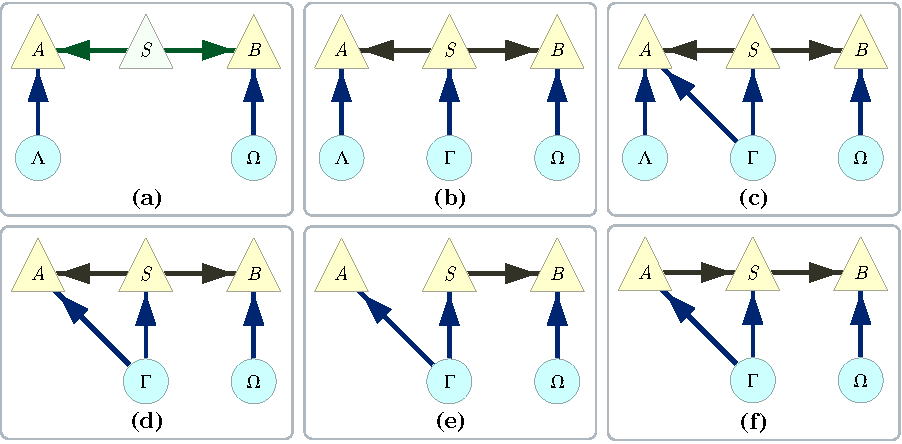
\includegraphics[width=\linewidth]{ObservationalEquivalencesExamples.pdf}
\caption{A set of observational equivalent causal structures. The reasons the changes are observational invariant are as follows: \\
(a)$\sim$(b) because $\Gamma$ is useless in (b), and as such $\Gamma$ can be dropped from (b) per \cref{theo:latentadding}.\\
(b)$\sim$(c) because $\NamedFunction{MB}{\!\Gamma\!}\subseteq\NamedFunction{pa}{\!A\!}$ in (b), and as such $\Gamma\to A$ can be added to (b) per \cref{theo:edgeadding}.\\
(c)$\sim$(d) because $\Lambda$ is redundant to $\Gamma$ in (c), and as such $\Lambda$ can be dropped from (c) per \cref{theo:latentadding}.\\
(d)$\sim$(e) because $\NamedFunction{pa}{\!S\!}\subseteq\NamedFunction{pa}{\!A\!}$ in (e), and as such $S\to A$ can be added to (e) per \cref{theo:edgeadding}.\\
(e)$\sim$(f) because $\NamedFunction{pa}{\!A\!}\subseteq\NamedFunction{pa}{\!S\!}$ in (e), and as such $A\to S$ can be added to (e) per \cref{theo:edgeadding}.
}\label{fig:equivalences}
\end{figure}

%Recall now the two steps of the transformation $\mathsf{ReduceToPCC}$. Imagine after the first step is finished, that an edge $A\to B$ remains, where $A$ is not a root node. Have directly connected all causal pathways, we know that $\NamedFunction{pa}{\!A\!}\subseteq\NamedFunction{pa}{\!B\!}$. As such, $\NamedFunction{pa}{\!B\!}\vDash A$, that is to say, $A$ is perfectly predictable given the parents of $B$. By \cref{theo:edgeadding}, therefore, if the edge $A \to B$ were not in the DAG, we would be able to add that edge without observational impact. By \cref{cor:edgedropping}, therefore, removing that edge has no observational impact. Indeed, the second step of $\mathsf{ReduceToPCC}$ leaves the post-first-step DAG observationally invariant. This allows us to quickly determine if a DAG is PCC-lossless.

%\begin{prop}\label{prop:PCClossless}
%A causal structure $G$ is PCC-lossless if every new edge in $\NamedFunction{ReduceToPCC}{\!G\!}$ relative to $G$ can be accounted for by adding edges to $G$ while leaving $G$ observationally invariant, pursuant to %\cref{theo:edgeadding,theo:latentadding}.
%\end{prop}

%%%%%%%%%%%% Enumeration via lowercase letters
\renewcommand{\labelenumi}{(\alph{enumi})}
\renewcommand{\theenumi}{(\alph{enumi})}
\renewcommand{\labelitemi}{$\circ$}



\section{Tobias's Original 7 Inequalities}

``I present several inequalities... together with a method of proof which has a combinatorial flavour. No quantum violations of any of these inequalities has been found to date."
%
%In the following the complement of a value is marked by an empty circle accent, so $\mathring{b}$ means ``anything but $b$", and accordingly $P(\mathring{a}\mathring{b})=P(A\mathopen{\neq}a,B\mathopen{\neq}b)$. 
%Additionally, an underscore stands for the corresponding marginal probability, like this: $P(\_b\_) := P(abc) + P(ab\mathring{c}) + P(\mathring{a}bc) + P(\mathring{a}b\mathring{c})$. 
\begin{theorem}
The following inequalities hold for all classical correlations in the triangle scenario:
\begin{enumerate}
\item
\(\quad
%--(a)--
%p(0\_\_)p(\_\_1) \leq p(00\_)+p(\_11)
p(a) p(c)  \leq  p(a b) + p(\nb c)
\)
\item
\(\quad
%--(b)--
%p(001) p(010) p(100)  \leq  p(000) + p(11\_) p(001) p(0\_\_) + p(1\_1) p(010) p(\_\_0) + p(\_11) p(100) p(\_0\_)
p(a b\nc) p(a \nb c) p(\na b c) \leq p(a b c) + p(\na \nb) p(a b \nc) p(a) + p(\na\nc) p(a\nb c) p(c)  + p(\nb \nc) p(\na b c) p(b)
\)
\item 
\(\quad
%--(c)--
%p(001) p(010) p(100) \leq  p(000)^2 + 2 p(11\_) p(001) + 2 p(1\_1) p(010) + 2 p(\_11) p(100)
p(a b\nc) p(a \nb c) p(\na b c) \leq p(a b c)^2 + 2\parens*{p(\na \nb) p(a b \nc) + p(\na\nc) p(a\nb c)  + p(\nb \nc) p(\na b c)}
\)
\item
\(\quad
%--(d)--
%p(000)^2 p(111)  \leq  p(001) p(010) p(100) + (2 p(000) + p(111)) (1 - p(000) - p(111))
p(a b c)^2 p(\na\nb\nc)  \leq  p(a b \nc) p(a \nb c) p(\na b c) + \parens*{2 p(a b c) + p(\na\nb\nc)} \parens*{1 - p(a b c) - p(\na\nb\nc)}
\)
\item
\(\quad
%--(e)--
%p(000)^2 p(111)  \leq  p(000)^3 + (2 p(000) + p(111)) (1 - p(000) - p(111))
p(a b c)^2 p(\na\nb\nc)  \leq  p(a b c)^3 + \parens*{2 p(a b c) + p(\na\nb\nc)} \parens*{1 - p(a b c) - p(\na\nb\nc)}
\)
\item
\(\quad
%--(f)--
%p(1\_\_)p(\_1\_)p(\_\_1) \leq p(000)+p(11\_)p(\_\_1)+p(1\_1)p(\_1\_)+p(\_11)p(1\_\_)
p(a) p(b) p(c) \leq  p(\na\nb\nc) + p(a b) p(c) + p(a c) p(b) + p(b c) p(a)
\)
\item
\(\quad
%--(g)--
%p(1\_\_)p(\_1\_)p(\_\_1) \leq p(000)^2+2 p(11\_)p(\_\_1) + 2 p(1\_1)p(\_1\_) + 2 p(\_11)p(1\_\_)
p(a) p(b) p(c) \leq  p(\na\nb\nc)^2 +2\parens[\Big]{ p(a b) p(c) + p(a c) p(b) + p(b c) p(a) }
\)
\end{enumerate}
\end{theorem}

It is quite likely that some of these inequalities are dominated by the others, but I do not know for sure whether any of them are actually redundant."

\purp{Note that \cref{eq:FritzF3} implies inequalities (a), (b), and (f). I haven't checked the others yet. \quoteby EW}


\section{Some of Elie's Triangle Scenario Inequalities}

The following inequalities follow from \cref{fig:Tri222} using linear quantifier elimination. The list is incomplete; longer inequalities have been excised in order to fit the page. A denser but complete list is embedded as the final page of this PDF. All the inequalities below are nontrivial, and are also unique under permutation of the parties or inverting outcomes. In expectation-value formation we imagine the two possible outcomes of each random variables to be $+1$ and $-1$.

\begin{align*}\def\arraystretch{1.5}
\hspace{-\mathindent}\begin{array}{l}
 0
\leq
{1 + \expec{A B} + \expec{A C} + \expec{B} \expec{C}} \\
 0
\leq
{2 -2 \expec{A C} + \expec{A} \expec{B} \expec{C} -\expec{C} \expec{A B}} \\
 0
\leq
{2 -\expec{A B C} + \expec{C} \expec{A B} + \expec{B} \expec{A C} + \expec{A} \expec{B C}} \\
 0
\leq
{2 + \expec{A B C} + \expec{C} \expec{A B} + \expec{B} \expec{A C} -\expec{A} \expec{B C}} \\
 0
\leq
{3 + \expec{A} + \expec{B} + \expec{C} + 3 \expec{A B} -\expec{A C} -\expec{B} \expec{C} + \expec{A} \expec{B} \expec{C} + \expec{C} \expec{A B} -\expec{B} \expec{A C}} \\
 0
\leq
{3 + \expec{A} + \expec{B} -\expec{C} + 3 \expec{A B} + \expec{A C} + \expec{B} \expec{C} + \expec{A} \expec{B} \expec{C} -\expec{C} \expec{A B} -\expec{B} \expec{A C}} \\
 0
\leq
{3 + \expec{C} -2 \expec{A B} -2 \expec{B C} + \expec{A} \expec{B} + \expec{A} \expec{B} \expec{C} -\expec{C} \expec{A B} -\expec{B} \expec{A C}} \\
 0
\leq
{3 + \expec{B} + \expec{A B} -2 \expec{B C} -\expec{A} \expec{B} + \expec{A} \expec{C} + \expec{A} \expec{B} \expec{C} + \expec{C} \expec{A B} -\expec{B} \expec{A C}} \\
 0
\leq
{3 + \expec{B} + \expec{A B} -2 \expec{B C} + \expec{A} \expec{B} -\expec{A} \expec{C} -\expec{A} \expec{B} \expec{C} + \expec{C} \expec{A B} + \expec{B} \expec{A C}} \\
 0
\leq
{3 -\expec{A} + \expec{B} + \expec{C} -\expec{A B C} + \expec{A} \expec{B} + \expec{A} \expec{C} -\expec{B} \expec{C} + \expec{A} \expec{B} \expec{C} + \expec{C} \expec{A B} + \expec{B} \expec{A C} + \expec{A}
   \expec{B C}} \\
 0
\leq
{3 + \expec{A} + \expec{B} -\expec{C} -2 \expec{A B} + \expec{A B C} + \expec{A} \expec{B} + \expec{A} \expec{C} + \expec{B} \expec{C} + \expec{A} \expec{B} \expec{C} + \expec{C} \expec{A B} + \expec{B} \expec{A C} -\expec{A} \expec{B C}} \\
 0
\leq
{4 + 2 \expec{C} -2 \expec{A B} -2 \expec{A C} -\expec{A B C} + 2 \expec{A} \expec{B} + 2 \expec{B} \expec{C} + \expec{C} \expec{A B} + \expec{B} \expec{A C} + \expec{A} \expec{B C}} \\
 0
\leq
{4 -2 \expec{B} -2 \expec{A B} -3 \expec{B C} + \expec{A B C} + \expec{B} \expec{C} + \expec{A} \expec{B} \expec{C} + \expec{C} \expec{A B} -\expec{B} \expec{A C}} \\
 0
\leq
{4 -2 \expec{C} -2 \expec{A B} -2 \expec{A C} -3 \expec{B C} + \expec{A B C} + 2 \expec{A} \expec{B} + \expec{B} \expec{C} -\expec{A} \expec{B} \expec{C} + \expec{C} \expec{A B} + \expec{B} \expec{A C}} \\
 0
\leq
{4 + 2 \expec{A B} -2 \expec{A C} + \expec{B C} + \expec{A B C} + 2 \expec{A} \expec{B} + 2 \expec{A} \expec{C} -\expec{B} \expec{C} -\expec{A} \expec{B} \expec{C} + \expec{C} \expec{A B} -\expec{B} \expec{A
   C}} \\
 0
\leq
{4 + 2 \expec{A B} -2 \expec{A C} + \expec{B C} + \expec{A B C} -2 \expec{A} \expec{B} + 2 \expec{A} \expec{C} -\expec{B} \expec{C} + \expec{A} \expec{B} \expec{C} + \expec{C} \expec{A B} + \expec{B} \expec{A C}}
   \\
 0
\leq
{4 -2 \expec{A B} + 3 \expec{B C} + \expec{A B C} + 2 \expec{A} \expec{B} + \expec{B} \expec{C} + \expec{A} \expec{B} \expec{C} -\expec{C} \expec{A B} -\expec{B} \expec{A C}} \\
 0
\leq
{4 -2 \expec{B} -2 \expec{A B} + \expec{A B C} -2 \expec{B} \expec{C} + \expec{C} \expec{A B} + \expec{B} \expec{A C} -\expec{A} \expec{B C}} \\
 0
\leq
{4 -2 \expec{A} -2 \expec{A B} -2 \expec{A C} + \expec{A B C} + \expec{C} \expec{A B} + \expec{B} \expec{A C} -\expec{A} \expec{B C}} \\
 0
\leq
{4 -2 \expec{C} -2 \expec{A B} -2 \expec{A C} -2 \expec{B C} + \expec{A B C} + 2 \expec{A} \expec{B} + \expec{C} \expec{A B} + \expec{B} \expec{A C} -\expec{A} \expec{B C}} \\
 0
\leq
{4 -2 \expec{A B} -2 \expec{A C} -2 \expec{B C} + \expec{A B C} + 2 \expec{A} \expec{B} + 2 \expec{A} \expec{C} + 2 \expec{B} \expec{C} + \expec{C} \expec{A B} + \expec{B} \expec{A C} + \expec{A} \expec{B C}} \\
 0
\leq
{5 + \expec{A} + \expec{B} + \expec{C} + 3 \expec{A B} + \expec{A C} -4 \expec{B C} -2 \expec{A} \expec{B} + \expec{B} \expec{C} + \expec{A} \expec{B} \expec{C} + \expec{C} \expec{A B} -\expec{B} \expec{A C}} \\
 0
\leq
{5 + \expec{A} + \expec{B} + \expec{C} + 3 \expec{A B} -\expec{A C} -4 \expec{B C} + 2 \expec{A} \expec{B} -2 \expec{A} \expec{C} + \expec{B} \expec{C} -\expec{A} \expec{B} \expec{C} + \expec{C} \expec{A B} +
   \expec{B} \expec{A C}} \\
 0
\leq
{5 + 3 \expec{A} + \expec{B} + \expec{C} + \expec{A B} + 3 \expec{A C} + \expec{B C} -\expec{A B C} + 2 \expec{A} \expec{B} + 2 \expec{A} \expec{B} \expec{C} -2 \expec{C} \expec{A B}} \\
 0
\leq
{5 + 3 \expec{A} + \expec{B} + \expec{C} + \expec{A B} + 3 \expec{A C} + \expec{B C} -\expec{A B C} + 2 \expec{A} \expec{B} -2 \expec{A} \expec{B} \expec{C} + 2 \expec{C} \expec{A B}} \\
 0
\leq
{6 -3 \expec{A B} -4 \expec{A C} + \expec{A} \expec{B} + 2 \expec{A} \expec{C} + 2 \expec{B} \expec{C} + \expec{A} \expec{B} \expec{C} -\expec{C} \expec{A B} -2 \expec{B} \expec{A C} -2 \expec{A} \expec{B
   C}} \\
 0
\leq
{6 + 2 \expec{B} + 3 \expec{A B} -4 \expec{A C} + \expec{A} \expec{B} + 2 \expec{A} \expec{C} + \expec{A} \expec{B} \expec{C} + \expec{C} \expec{A B} -2 \expec{B} \expec{A C} -2 \expec{A} \expec{B C}} \\
 0
\leq
{6 -2 \expec{A} + 2 \expec{B} -3 \expec{A B} -5 \expec{A C} + \expec{A} \expec{B} + \expec{A} \expec{C} + 2 \expec{A} \expec{B} \expec{C} + \expec{C} \expec{A B} -\expec{B} \expec{A C} -2 \expec{A} \expec{B
   C}} \\
 0
\leq
{6 -3 \expec{A B} + \expec{A C} -2 \expec{B C} + \expec{A} \expec{B} + \expec{A} \expec{C} -4 \expec{B} \expec{C} + 2 \expec{A} \expec{B} \expec{C} + \expec{C} \expec{A B} -\expec{B} \expec{A C} -2 \expec{A}
   \expec{B C}} \\
 0
\leq
{6 + \expec{A B} -3 \expec{A C} + 2 \expec{B C} + \expec{A} \expec{B} + \expec{A} \expec{C} -4 \expec{B} \expec{C} -2 \expec{A} \expec{B} \expec{C} + \expec{C} \expec{A B} -\expec{B} \expec{A C} -2 \expec{A}
   \expec{B C}} \\
 0
\leq
{6 + 2 \expec{C} + 3 \expec{A C} -5 \expec{B C} -2 \expec{A} \expec{B} + \expec{A} \expec{C} + \expec{B} \expec{C} -2 \expec{A} \expec{B} \expec{C} + 2 \expec{C} \expec{A B} + \expec{B} \expec{A C} + \expec{A}
   \expec{B C}} \\
 0
\leq
{6 -3 \expec{A B} -2 \expec{A C} -2 \expec{B C} -2 \expec{A B C} + \expec{A} \expec{B} + 4 \expec{B} \expec{C} + \expec{A} \expec{B} \expec{C} -\expec{C} \expec{A B} -2 \expec{B} \expec{A C}} \\
\end{array}
\end{align*}

\clearpage
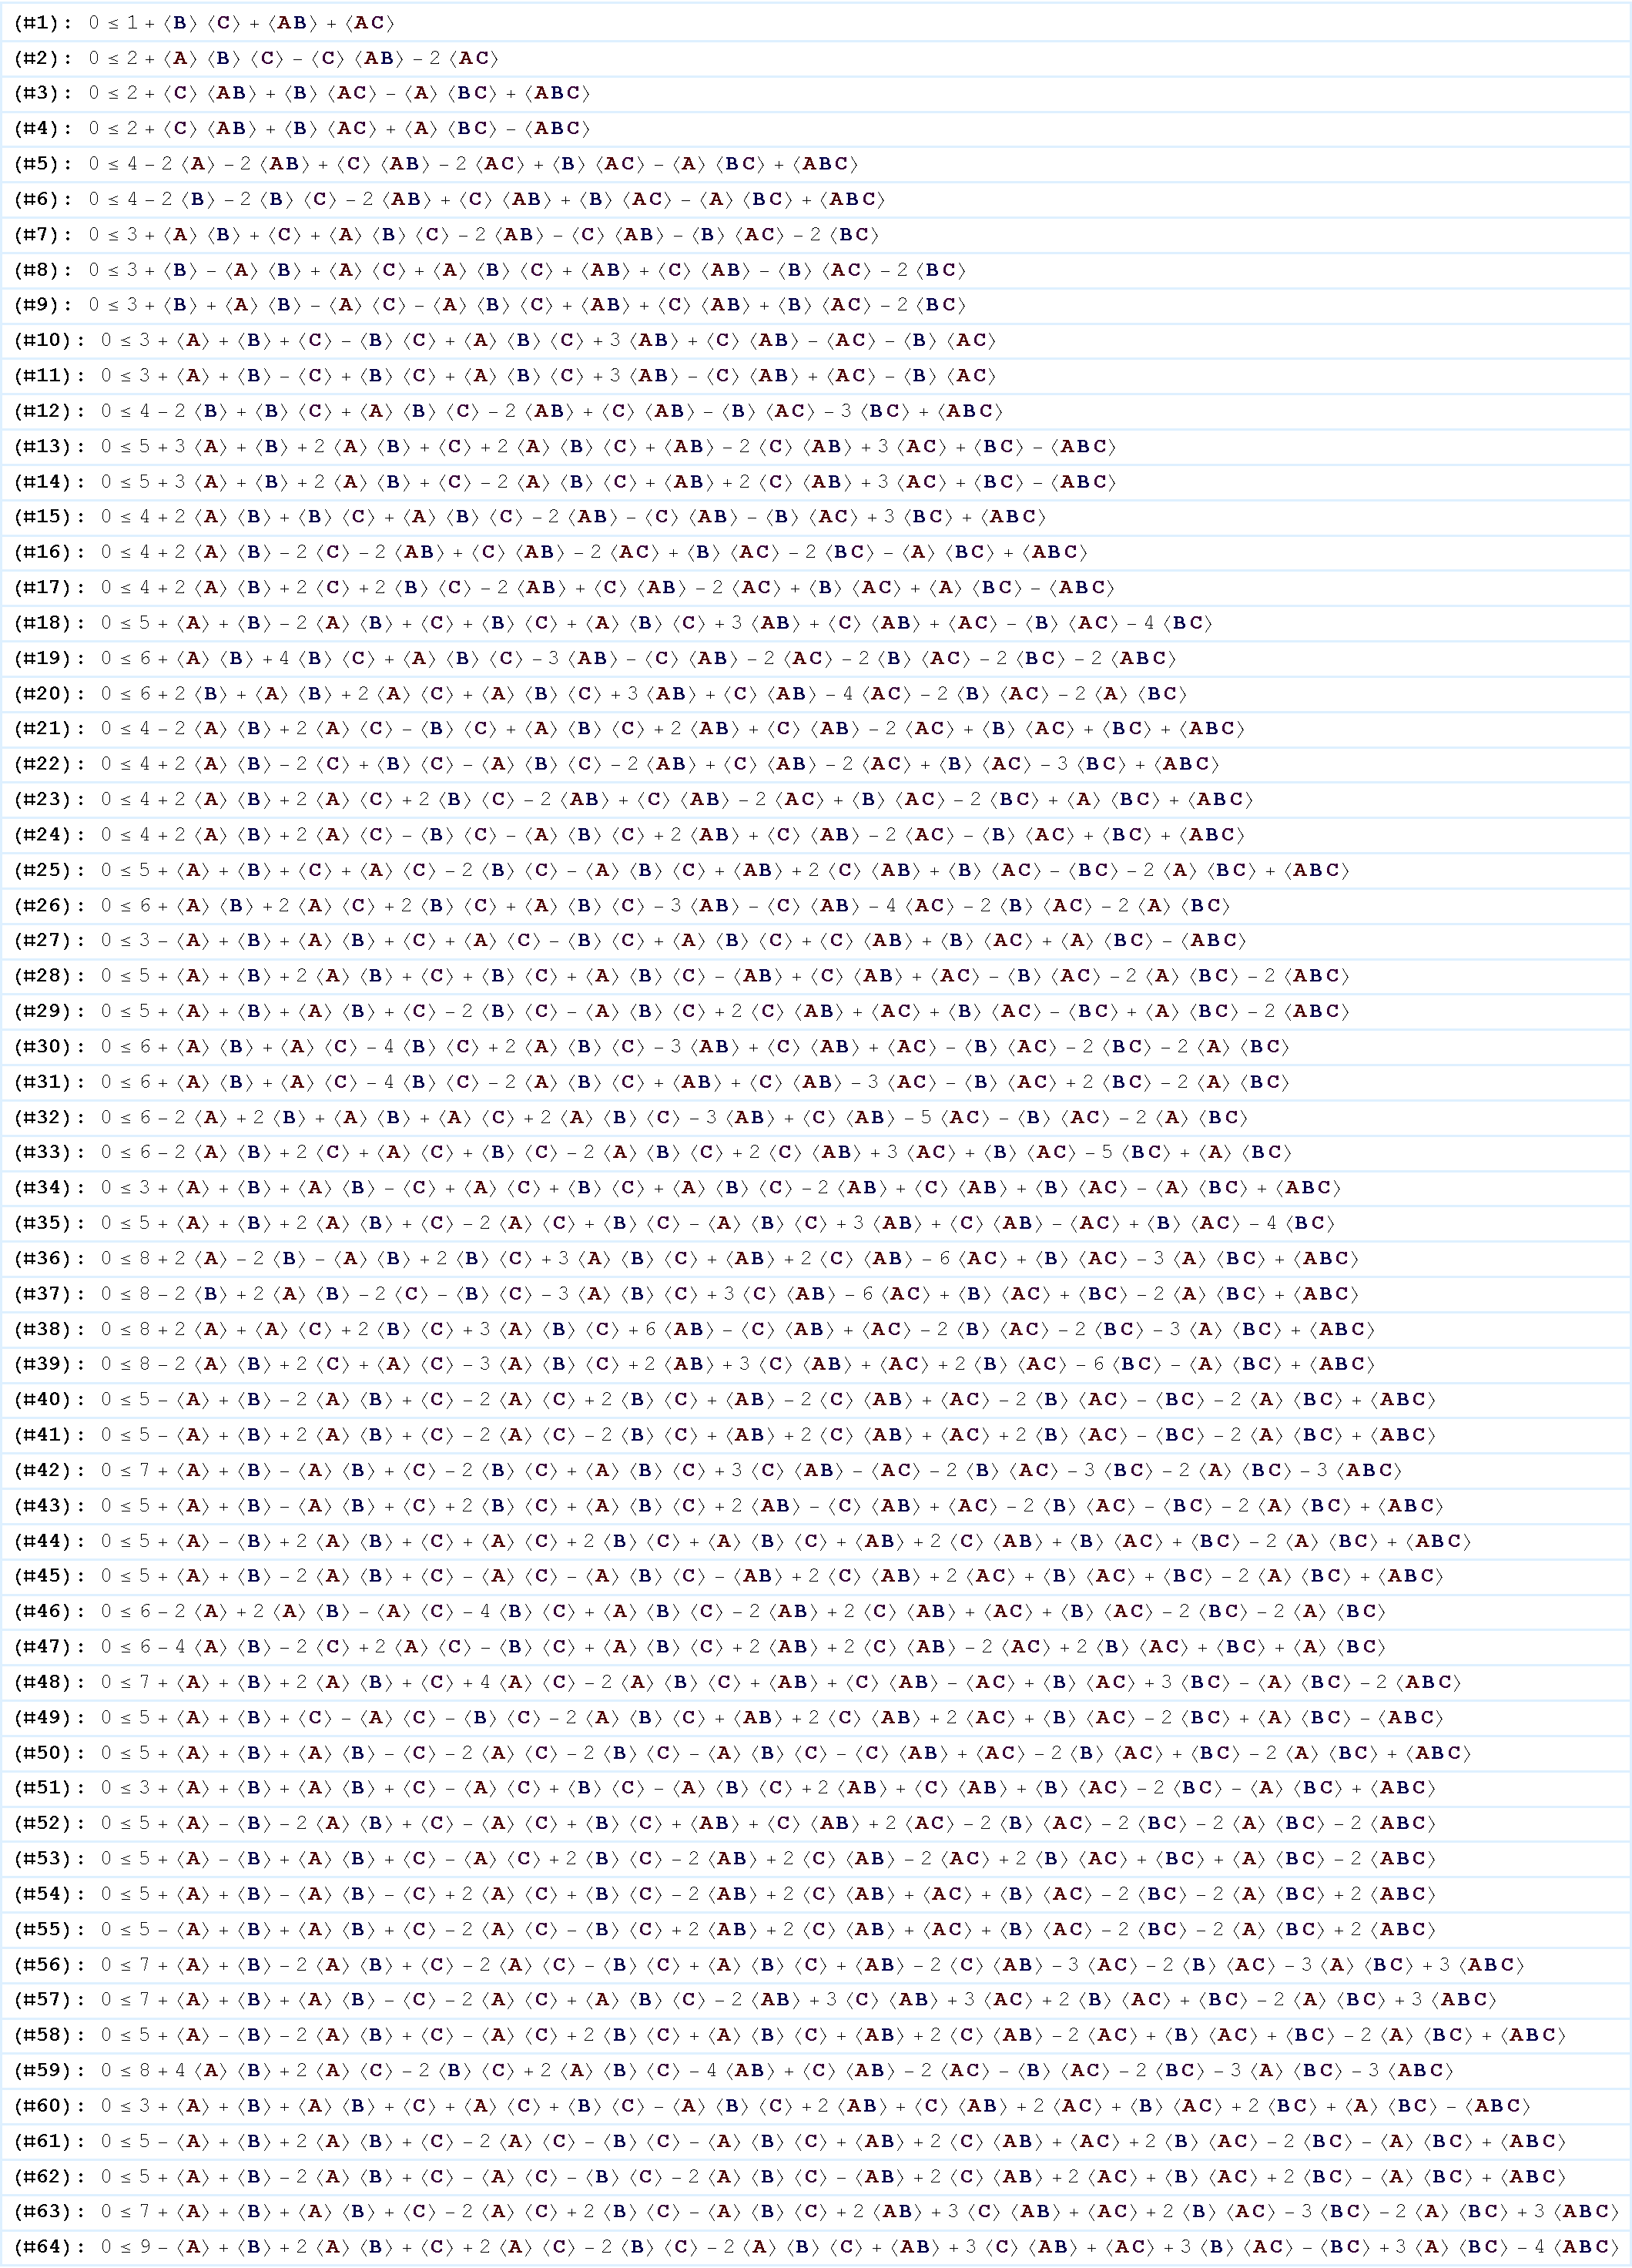
\includepdf[pages=-]{64InequalitiesForTobias.pdf}

%\section*{References}
%\nocite{*}
%\setlength{\bibsep}{\smallskipamount}
%\clearpage
\setlength{\bibsep}{3pt plus 3pt minus 2pt}
\bibliographystyle{apsrev4-1}
\nocite{apsrev41Control}
\bibliography{hardyinference}

\end{document}

\color{blue} A causal model consists of a pair of objects: a causal structure and a set of parameters.  The causal structure is a directed acyclic graph (DAG).  Recall that a DAG $G$ consists of a set of nodes and directed edges (i.e., ordered pairs of nodes), which we denote by $\SmallNamedFunction{Nodes}{G}$ and $\SmallNamedFunction{Edges}{G}$ respectively.  Physically, each node in the DAG corresponds to a localized system and a directed edge between two nodes corresponds to there being a direct causal influence from one system to the other.  The parameters specify, for each root node, how the system corresponding to that node is prepared, and for each node that has parents in the DAG, the precise manner in which it causally depends on its parents.  If a DAG is denoted $G$ and the parameters thereon are denoted $\mathcal{P}(G)$, then the corresponding causal model is the pair $C = (G,\mathcal{P}(G))$.  We shall also make use of the notation $\SmallNamedFunction{DAG}{C}$ for $G$ and $\SmallNamedFunction{Params}{C}$ for $\mathcal{P}(G)$.

In a {\em classical} causal model, the localized systems are random variables, and the parameters are probabilities and conditional probabilities on these random variables.  Specifically, for each root node, the model specifies a probability distribution over the values of the associated random variable, and for each non-root node, it specifies a conditional probability distribution over the values of the random variable associated to that node, given the values of the variables associated to its parents in the DAG.  Denoting the conditional probability distribution associated to a node $A$ in the DAG $G$ by $P_G(A|{\rm Pa}(A))$, we have
\begin{align}
\mathcal{P}(G) \equiv \{ P_G(A|{\rm Pa}(A)): A \in \SmallNamedFunction{Nodes}{G}\}.
\end{align}
Note that the root nodes are included as those for which the parents are the null set and the conditional probability distribution is simply a probability distribution.

Classical causal models will be the primary focus of this article. Nonetheless, there is a quantum generalization of the notion of a causal model that will feature in our discussions at the end of this article.  In a {\em quantum} causal model\cite{leifer2013conditionalstates}, the localized systems are types of quantum systems (specified by Hilbert space dimensionality), and the parameters are quantum operations.  Specifically, for each root node, the model specifies a unit-trace positive operator on the Hilbert space for that system and for each non-root node, the model specifies a trace-preserving completely-positive linear map from the operators on the Hilbert space of the parents of the system to the operators on the Hilbert space of the system.  Certain nodes in a quantum causal model may be considered classical, in which case all states and operations must be diagonal in some fixed basis on that system.  One can also generalize the notion of a causal model further still to the case of generalized probabilistic theories, as was done in Ref.~\cite{pusey2014gdag}.
 %random variable\footnote{In the quantum context, however, only \emph{observable} nodes correspond to classical random variables, such as the outcomes of measurements. Latent nodes, however, represent quantum systems. Functional dependence is replaced by the action of a quantum operation, and edges then dictate the ways in which quantum systems factor and/or compose. See Refs. \cite{pusey2014gdag,leifer2013conditionalstates}. \purp{Rob, add appendix? Classical/Quantum/GPT everything? I'm thinking a table would be nice.}}, while each edge represents a possible causal influence between variables. 

When a causal model constitutes a hypothesis for explaining a probability distribution over a set of observed variables, then it is natural to distinguish the nodes in the DAG that correspond to observed variables and those that correspond to unobserved variables.  As is standard, the only unobserved variables worth incorporating into one's DAG are those that act as common causes of observed variables.  These are termed {\em latent variables}.  In our graphical depictions of the DAG, we follow the convention of representing the latent nodes by circles, and observable nodes by triangles \cite{pusey2014gdag}.

A causal inference problem is one whose input is some observed data---for instance, a sample of the probability distribution over the observed variables, or some coarse-grained properties thereof---and whose output is a verdict on (or probabilistic inference about) whether a given causal model can explain the observed data.   The particular causal inference problem that is most widely studied is one wherein there is no constraint on the set of parameters that supplements the given causal structure.  Another version of the problem, however, seeks to determine whether the given causal structure can explain the observed data when certain parameters are constrained to be of a particular form.  For instance, the parameters might be constrained to describe a particular type of functional dependence of some variable on its parents.  An example is the assumption of an additive noise model [provide references].

The inflation DAG technique that we introduce will define a novel sort of constraint on the parameters of a causal model.  We pause to describe this constraint in general terms, before introducing the notion of inflation.  The sorts of causal structures that can arise in our inflation scheme have the property that necessarily there will be certain pairs of variables which have the same ancestral subgraph.  The constraint on the parameters is that the two conditional probability distributions describing how each variable of the pair depends on its parents are quantitatively equal to one another.  (To our knowledge, this sort of constraint has not been considered before in causal inference.)

{\bf Describing the hard problem, which, if it were solved, would exhaust what one can infer from the inflation DAG technique.}

We now introduce the notion of \tblue{the inflation of a causal model}.  We describe what inflation means for the causal structure and the parameters.  Let $C=(G,\mathcal{P}(G))$ denote the original causal model and $C'=(G',\mathcal{P'}(G'))$ its inflation.

For $C'$ to be an inflation of $C$, the DAG $G'$ must be related to $G$ as follows:  (i) For each node of $G$, $G'$ contains one or more copies of that node. If $A$ denotes a node in the DAG $G$, then we denote its copies in the inflation DAG $G'$ by $A_1,\ldots, A_k$.  The variable that indexes the copies is termed {\em the copy-index}, and a set of variables in $G'$ that differ only by copy-index are called a {\em copy set} and we denote the set of these by $\SmallNamedFunction{CopySets}{G'}$; (ii) the ancestral subgraph in $G'$ of a node $A_i$ is equivalent, under removal of the copy-index, to the ancestral subgraph in $G$ of the node $A$.  

When two objects (e.g.~nodes, sets of nodes, DAGs, etc\ldots) are the same up to copy-indices, then we use $\sim$ to indicate this, so $A_i\sim A_j\sim A$.  Given this notational convention, we can formalize the condition for $G'$ to be the DAG for an inflation of a causal model with DAG $G$ as follows:
\begin{align}\label{eq:definflationDAG}
%\forall A \in \SmallNamedFunction{Nodes}{G}, ???\nonumber\\
G' \in\SmallNamedFunction{Inflations}{G} \quad\text{ iff }\quad \forall A_i\in \SmallNamedFunction{Nodes}{G'}:\; \ansubgraph[G']{A_i}\sim\ansubgraph[G]{A}.
\end{align}

Note that this implies that if $G'$ is a DAG arising from inflation, then certain subgraphs of $G'$ are identical,
\begin{align}\label{eq:ConstraintOnInflationDAG}
\forall S \in \SmallNamedFunction{CopySets}{G'}: A_i,A_j \in S \implies \ansubgraph[G']{A_i}\sim\ansubgraph[G]{A}.
\end{align}


Furthermore, For the causal model $C'$ to be an inflation of the causal model $C$, the parameters $\mathcal{P'}(G')$ must be related to the parameters $\mathcal{P}(G)$ as follows: 
For every node $A_i$ in $G'$, the manner in which $A_i$ causally depends on its parents within $G'$ must be the same as the manner in which $A$ causally depends on its parents within $G$.   Formally, 
\begin{align}\label{eq:funcdependences}
\forall A_i \in \SmallNamedFunction{Nodes}{G'}:\; \pdf{A_i| {\rm Pa}_{G'}(A_i)}=\pdf{A|{\rm Pa}_{G}(A)}.
\end{align}

Note that this implies that if $\mathcal{P}(G')$ are the parameters of a causal model arising from inflation, then these are constrained relative to the set of possible parameters that could be defined for a DAG $G'$.  The constraint is:
\begin{align}\label{eq:ConstraintOnFuncdependences}
\forall S \in \SmallNamedFunction{CopySets}{G'}: A_i,A_j \in S \implies \pdf{A_i| {\rm Pa}_{G'}(A_i)}=\pdf{A_j|{\rm Pa}_{G'}(A_j)}.
\end{align}

It is worth emphasizing the significance of the latter constraint.  Let the set $\mathcal{C}_G$ be the set of all causal models associated with a DAG $G$, which is to say the set of pairs $(G, \mathcal{P}(G))$ wherein $\mathcal{P}(G)$ are a set of valid conditional probabilities, 
\begin{align}
\mathcal{C}_G \equiv \{ C: \SmallNamedFunction{DAG}{C} =G\}.
\end{align}
Let the set of causal models $\mathcal{C}'_{G'}$ be the image of $\mathcal{C}_G$ under some nontrivial inflation map.  $\mathcal{C}'_{G'}$ is {\em not} the set of all causal models associated with $G'$ but rather the subset that satisfy Eq.~\eqref{eq:ConstraintOnFuncdependences}.


